\include{Macros/MacroFile1}

\documentclass[twoside,11pt]{Classes/myThesis}


%%%%%%%%%%%%%%%%%%%%%%%%%%%%%%%%%%%%%%%%%%%%%%%%%%%%%%
%%%%%%%%%%%%%%% file path for figures - add extra chapters as necessary %%%%%%%%%
%%%%%%%%%%%%%%%%%%%%%%%%%%%%%%%%%%%%%%%%%%%%%%%%%%%%%%
\graphicspath{{./Chapters/Chapter_1/Chapter_1_Fig/}     
              {./Chapters/Chapter_2/Chapter_2_Fig/}
              {./Chapters/Chapter_2a/Chapter_2a_Fig/}
              {./Chapters/Chapter_2b/Chapter_2b_Fig/}
              {./Chapters/Chapter_3/Chapter_3_Fig/}
              {./Chapters/Chapter_4/Chapter_4_Fig/}
              {./Chapters/Chapter_5/Chapter_5_Fig/}
              {./ThesisFigs/}}

%%%%%%%%%%%%%%%%%%%%%%%%%%%%%%%%%%%%%%%%%%%%%%%%%%%%%%
%%%%%%%%%%%%% Constants - fill these in for use throughout the thesis %%%%%%%%%%%%
%%%%%%%%%%%%%%%%%%%%%%%%%%%%%%%%%%%%%%%%%%%%%%%%%%%%%%
\newcommand{\theAuthor}{Rodrigo Daniel Solis Ortega}
\newcommand{\authorEmail}{el14rdso@leeds.ac.uk}
\newcommand{\myTitle}{Modelling and characterization of soft materials for bioinspired series-elastic actuators}
%%%%%%%%%%%%%%%%%%%%%%%%%%%%%%%%%%%%%%%%%%%%%%%%%%%%%%
\pdfinfo { /Title  (\myTitle)
           /Creator (TeX)
           /Producer (pdfTeX)
           /Author (\theAuthor \authorEmail)
           /ModDate (D:\pdfdate)
           /CreationDate (D:\pdfdate)  %format D:YYYYMMDDhhmmss
           /Subject (Condensed Matter Physics)
           /Keywords (PhD, Thesis)}    
		\pdfcatalog { /PageMode (/UseOutlines)
                  /OpenAction (fitbh)  }

%%%%%%%%%%%%%%%%%%%%%%%%%%%%%%%%%%%%%%%%%%%%%%%%%%%%%%
%%%%%%%%%%%%% Title Page Information %%%%%%%%%%%%%%%%%%%%%%%%%%%%
%%%%%%%%%%%%%%%%%%%%%%%%%%%%%%%%%%%%%%%%%%%%%%%%%%%%%%
\title{\myTitle}
\author{\href{mailto:\authorEmail}{\theAuthor}}
\crest{\includegraphics[width=35mm]{Leeds_Crest.png}}
%%%%%%%%%%%%%%%%%%%%%%%%%%%%%%%%%%%%%%%%%%%%%%%%%%%%%%
%% Define these as empty to omit the two logos on the title page
%%%%%%%%%%%%%%%%%%%%%%%%%%%%%%%%%%%%%%%%%%%%%%%%%%%%%%
\logo{\includegraphics[width=50mm]{UoL_logo}} %University Logo
\deptlogo{} %\includegraphics[width=50mm]{UoL_logo}} % Institute Logo
%%%%%%%%%%%%%%%%%%%%%%%%%%%%%%%%%%%%%%%%%%%%%%%%%%%%%%
\collegeordept{\href{https://engineering.leeds.ac.uk/mechanical}{Institute of Design, Robotics and Optimization \\* School of Mechanical Engineering}}
\university{\href{http://www.leeds.ac.uk}{University of Leeds}}

\degree{Doctor of Philosophy}
\degreedate{\monthdate\today}

%Different font in caption
%%%%%%%%%%%%%%%%%%%%%%%%%%%%%%%%%%%%%%%%%%%%%%%%%%%%%%
%%%%%%%%%%%%%%%% Optional Packages  %%%%%%%%%%%%%%%%%%%%%%%%%%%
%%%%%%%%%%%%%%%%%%%%%%%%%%%%%%%%%%%%%%%%%%%%%%%%%%%%%%
%\usepackage{StyleFiles/watermark}
\usepackage{xspace}  %add a space after maths if not already there
%\usepackage{booktabs} %better tables
%\usepackage{rotating}  %rotating figures and tables
\usepackage{array} %enhanced tables
%\usepackage{ctable} %include a figure command
%\usepackage{footnote}
\usepackage{multirow} %for merging cells on tables
%\usepackage{times} % The "Times" font
%\usepackage{Utopia} % The "Utopia" font
\usepackage[toc,page]{appendix}
\usepackage{caption}
\usepackage{subcaption} %This solve the error caused with subfigure
\usepackage{float}
\usepackage{hyperref}
\usepackage[ruled,vlined]{algorithm2e}


%User Definitions
\newcolumntype{C}[1]{>{\centering\arraybackslash}p{#1}}

\linespread{1.3} %1.5 line spacing

\begin{document}

\maketitle

%set the number of sectioning levels that get number and appear in the contents
\setcounter{secnumdepth}{3}
\setcounter{tocdepth}{3}
%Make the label printed by autoref be section for subsection and subsubsection
\let\subsectionautorefname\sectionautorefname
\let\subsubsectionautorefname\sectionautorefname
\pagenumbering{roman}
\frontmatter

%Insert empty page after title
\newpage\null\thispagestyle{empty}\newpage

%%%%%%%%%%%%%%%%%%%%%%%%%%%%%%%%%%%%%%%%%%%%%%%%%%%%%%
%%%%%%%%%%%% Include sections are required, or comment out to skip over %%%%%%%%%
%%%%%%%%%%%%%%%%%%%%%%%%%%%%%%%%%%%%%%%%%%%%%%%%%%%%%%
%\include{Dedication/dedication}
% Thesis IP Statement ---------------------------------------------------

\begin{ipstatement}
The candidate confirms that the work submitted is his own, except where work which has formed part of jointly authored publications has been included. The contribution of the candidate and the other authors to this work has been explicitly indicated below. The candidate confirms that appropriate credit has been given within the thesis where reference has been made to the work of others.
\\
\\
\hyperref[sec:characterizationKKP]{Section~\ref*{sec:characterizationKKP}} of this thesis is based on a jointly-authored conference paper: \textit{Solis-Ortega, R.D., Dehghani-Sanij, A.A. and Martinez-Hernandez, U., 2017, July. Characterization of kinetic and kinematic parameters for wearable robotics. In Annual Conference Towards Autonomous Robotic Systems (pp. 548-556). Springer, Cham.}.
\\
\\
\Cref{sec:ChapterModellingLVM} of this thesis is based on a jointly-authored conference paper: \textit{Solis-Ortega, R.D., Dehghani-Sanij, A.A. and Martinez-Hernandez, U., 2018, August. The assessment of viscoelastic models for nonlinear soft materials. In 2018 7th IEEE International Conference on Biomedical Robotics and Biomechatronics (Biorob) (pp. 1274-1279). IEEE.}.
\\
\\
The contributions of the candidate to these papers include the literature review, data collection, design and execution of simulation, statistical analysis, and writing. The contribution of the other authors to these papers include guidance, supervision, and revision.
\\
\\
This copy has been supplied on the understanding that it is copyright material and that no quotation from the thesis may be published without proper acknowledgement.
\\
\\
The right of \theAuthor{} to be identified as Author of this work has been asserted by him in accordance with the Copyright, Designs and Patents Act 1988.
\\
\\
\copyright{} \yeardate{\today} The University of Leeds and \theAuthor{}.

\label{ips}
\end{ipstatement}

% ----------------------------------------------------------------------

%%% Local Variables: 
%%% mode: latex
%%% TeX-master: "../thesis"
%%% End: 

% Thesis Acknowledgements ------------------------------------------------


%\begin{acknowledgementslong} %uncommenting this line, gives a different acknowledgements heading
\begin{acknowledgements}      %this creates the heading for the acknowlegments

\setlength{\parindent}{17.62482pt}
\setlength{\parskip}{0.0pt plus 1.0pt}

\textit{I would like to thank to both Professor Abbas Dehghani-Sanji and Dr Uriel Martinez Hernandez who have guided me on the pursue of a PhD. As well as the many people who directly or indirectly were involved in this personal goal. I would like to thank my family for always being extremely supporting and to my financial sponsor, CONACYT.}

\end{acknowledgements}
%\end{acknowledgmentslong}

% ------------------------------------------------------------------------

%%% Local Variables: 
%%% mode: latex
%%% TeX-master: "../thesis"
%%% End: 


% Thesis Abstract -----------------------------------------------------


%\begin{abstractslong}    %uncommenting this line, gives a different abstract heading
\begin{abstracts}        %this creates the heading for the abstract page

\setlength{\parindent}{17.62482pt}
\setlength{\parskip}{0.0pt plus 1.0pt}
	
This emerging field of soft robotics is currently being applied for human assistance applications such as soft orthoses or soft exosuits able to assist human movements. The elder people is main sector of the population which will be directly benefited by the development of a portable, compliant, lightweight and efficient soft exosuit. Current developments rely on well established technologies such as pneumatic artificial muscles and electric motors paired with Bowden cables. However, many research is aiming on improving both the established technologies and emerging technologies such as shape memory materials. The current report describes the state of the mentioned field of interest while paying particular attention to the soft actuation technologies advantages, limitations and proposed improvements. In a similar way, the soft perception technology is as well discussed along the control techniques being implement-ed in soft exosuits and soft orthoses. Furthermore, the development of a hybrid soft actuator is proposed by combining two or more available technologies in an attempt to overcome their individual limitations. Moreover, as a preliminary design step, it is described the characterization of the parameters for the human lower limb for daily living activities which aims to provide the information required to tailor the hybrid soft actuator design parameters. The characterization considers four main daily activities: walking, using steps, walking on a ramp and using a chair. In the same way, the parameters of torque, angle and power during such activities were recorded from several clinical trials and plotted for analyzing. Through the obtained charts it is possible to define the required parameters of the soft hybrid actuator to be designed. Finally, as a preliminary experimental work, the feasibility of imitating the musculoskeletal-tendon system is assessed by characterizing the mechanical properties of polyethylene rubber, since the literature suggest that this type of material have similar properties as the human tendon.

\end{abstracts}
%\end{abstractlongs}

% ----------------------------------------------------------------------

%%% Local Variables: 
%%% mode: latex
%%% TeX-master: "../thesis"
%%% End: 

\tableofcontents
\listoffigures
\let\cleardoublepage\clearpage
\listoftables
\let\cleardoublepage\clearpage
\include{Abbreviations/Abbreviations}
\include{Common_Symbols/Common_Symbols}

\mainmatter

\pagenumbering{arabic}
\chapter{Introduction}
\section{ Background}

\Large{The background must give an overview of the current development, the progress of the research and the gaps in knowledge (research opportunities) }

The field of Soft robotics deals with the implementation of soft and deformable materials in traditional Robotics applications. The interest and research in this field has increased in the past decade. The latter is due to the outstanding developments in terms of manufacturing of soft materials, such as elastomers, and the development of new soft materials which can be stimulated, i.e. deformed, by heat, light, and magnetism. 

The coordination action called RoboSoft, supported by the IEEE Robotics and Automation Society (RAS) and the European Commission, has played a very important role in spreading the awareness of the wide number of Soft Robotics applications. The RoboSoft committee formally defines the field of Soft Robotics as ``Soft robot/devices that can actively interact with the environment and can undergo `large' deformations relying on inherent or structural compliance'' \cite{laschi2016soft}. The categorization of when a robotic application fall into the field of Soft Robotics depends on the material's Young Modulus, a mechanical property which relates the material's deformation with the amount of stress applied to it; which must be between the range of 10$^{2} - $10$^{6}$ Pascals (Pa). The Young's modulus is usually a measure of a solid material stiffness; a high value refers to a stiff material in the same way as a low value refers to an elastic or soft material. In the context of Soft Robotics, the term compliance it is most used instead of stiffness since it refers to the adaptability of the material under certain circumstances.

Early applications in Soft Robotics were inspired in nature, by observing that most biological organisms are not rigid, e.g. the human skeleton only contributes with 11\% of an adult's weight, on contrast, the skeletal muscle in our body only contributes with 42\% of the weight \cite{kim2013soft}. This inspiration gave birth to several soft bio-inspired robots, as well as the interest in studying the embodied intelligence of biological organisms. The latter refers to the ability of biological organisms to adapt to different situations by exploding their body morphology and properties. This is one of the main differences between soft and rigid robots. The embodied intelligence of soft robots release the controller from the task of accurately controlling the position of the robot and of constantly monitoring the working environment; allowing the controller to focus on the execution of commands. This is only possible with the implementation of soft and deformable materials able to automatically adapt to perturbations from the environment, such as uneven terrains and obstacles. Bio-inspired soft robots are now being developed for a broad range of applications, such as locomotion, manipulation, and even replicating biological processes such as digestion. The research done in the field of Soft Robotics has an interesting multidisciplinary potential. For example, the locomotion of caterpillars and snake could be study by building a soft robot which replicates this motion. The knowledge extracted from this could be useful for the development of actuated bendable soft cylinders which ultimately could replace the current rigid tools being used in laparoscopic surgery \cite{rus2015design}.

The mechanical behaviour of soft materials, is very difficult to model using traditional mathematical models, due to their non-linear, time-dependent and strain-rate-dependent stress response. This great challenge motivated the research in Soft Robotics to develop bio-inspired soft bodies, arms and legs able to perform the task at hand using minimal control. This caused a shift in the traditional design approach for rigid robots from ``rigidity by design, safety by sensors and control'' to design approach used in soft robots, ``safety by design, performance by control''. The added feature of safety, inherent in most soft robots, allowed the development of Physical Human-Robot Interaction (PHRI) applications \cite{filippini2008toward}. Many other challenges face by this emerging field are listed in \cite{laschi2016soft,trivedi2008soft} being: actuation of soft materials, development and implementation of soft sensors into soft robots, control systems able to deal with the nonlinear behaviour of soft materials, and modelling tools able to accurately predict the mechanical behaviour of soft materials in real-time. Most of these limitations come from the simple fact that soft robots cannot be considered as a chain of rigid links able to rotate or slide as common robots are, but soft robots are deformable and continuous which means that all the foundation in which Robotics is based on, is not easily transferable to the Soft Robotics field. 

The design and development of soft robots is very challenging, however, the potential benefits are many \cite{iida2011soft}. Foe example, soft robots have the potential of being very dexterous due to the ability of modifying their shape depending on the environment; soft robots can can manipulate objects of different shapes, sizes, and most importantly they are safe to interact with humans in the event of an unplanned collision. The latter benefits highlight the potential of Soft Robotics for PHRI applications such as, orthoses, surgical tools, and wearable devices. This research aims to contribute to the technological advance of Soft Robotics for human assistance applications.

For a long time, humans have pursued the idea of increasing their strength, stamina and speed through different means. Currently, we are relaying on technological advances to achieve the latter by building wearable robotic devices, commonly known as robotic exoskeletons. This wearable device was motivated by military applications where a soldier is required to carry a heavy load in its back for a long period of time, ultimately causing him injuries or early fatigue. The robotic exoskeleton is able to carry a payload and transmit the payload weight to the ground, ideally relieving the wearer from feeling the payload, which allows the wearer to walk greater distances without premature fatigue. The rigid nature of these devices and the big actuators implemented to achieve forces able to enhance humans, impose many limitations, such as, restriction of body movements, interference on subject natural biomechanics and high inertia which impedes the device to follow the subject intentions smoothly, creating a drag feeling \cite{asbeck2014stronger}.

In the field of Soft Robotics, research is being done to develop a soft version of a robotic exoskeleton, formally called soft exosuit, in an attempt to solve the previously mentioned limitations. Soft exosuits are wearable robotic systems meant to be worn in the same way as clothes, by attaching both the actuation and perception systems into a wearable structure, made of textiles, strapped to the human body which will ultimately assist the wearer's motions. Despite the many benefits of this technology, in comparison to the robotic exoskeleton, current developments of soft exosuits are not able to deliver enough mechanical power to be called an enhancement device. Currently, soft exosuits are considered an assistive device. This limitation is inherent from the idea of having a soft wearable device. The conversion of forces and torques, generated by the actuators attached to a wearable textile or directly to the user's body, into useful assistive torques for human joints assistance is very challenging. In a rigid exoskeleton the reaction forces produced by the actuators are sustained by the exoskeleton mechanical frame, but this is not the case in soft exosuits, where the reaction forces must be dissipated through the worn textile attached to the human body, which generates uncomfortable frictions between the user skin and the textile. Nevertheless, the human body naturally possesses areas able to sustain high amounts of forces, these areas are currently being exploited into soft exosuit designs to prevent discomfort, skin injury, and to increase the efficiency of transmitted forces. The latter principle is implemented in \cite{wehner2013lightweight} where a lower limb soft exosuit using pneumatic muscles is developed. The other, most common approach is to fix a wearable soft material to the skin, as in \cite{park2014design,park2011bio} where pneumatic artificial muscles (PAM) were attached to a soft cloth and disposed in such a way that they can mimic the biological musculoskeletal behaviour of a human foot. Among the available soft exosuit developments, few of them implements a closed loop control system, due to the high complexity of dealing with the non-linearity of soft materials. 

%On the other hand, several works focus on the characterization and testing of soft technologies as \cite{wehner2012exp} where an accurate characterization of a PAM is performed, which directly contribute to the development of previously mentioned soft exosuits. Many other technologies are being researched as well, such as, shape memory alloys (SMAs), which are metal alloys capable of changing its form when  properly stimulated. One of the main drawbacks of this technology is the amount of energy and time required to heat metal alloy and activate its shape shifting ability. The latter limitation is highlighted in \cite{Stirling2011}, where soft orthoses for foot and knee were developed SMA springs embedded in a soft fabric. The response of the device was to slow to be used for human assistance. Another commonly implemented actuation technology are cable-driven actuators, typically consisting of an electric motor and a Bowden cable. This electromechanical system create pulling forces by applying tension to a cable fixed in two different points. The cables must be routed along the body of the wearer to deliver the acting force to the joint of interest \cite{asbeck2013biologically,asbeck2015biologically}. The stroke length is not limited in this type of technology, as is the case for PAMs, since Bowden cables are flexible and can be routed in many different ways.

%Many soft sensing technologies have also been developed, being hyper-elastic strain sensors the most common one, which are based on the change in resistance of a liquid metal alloy inside conducts embedded into an elastic polymer which allows the measurement of the body limb position and sustained forces; its performance allowed the development of a soft artificial skin \cite{park2012design}. This technology was later implemented in a soft exosuit to allow for the measurement of the human biomechanics. A comparison analysis between the latter approach and the well-established motion capture technology was performed in \cite{mengucc2014wearable}, where the implementation of strain sensors to capture the human biomechanics showed remarkable results.

The progress in the field of Soft Robotics has been very quick and very diverse. Most of the research is focused on studying the benefits of using a specific new soft material in a robotic application, leaving the control system on a second plane. This is mostly due to the complexity of developing a modelling tool to accurately predict the mechanical behaviour of soft materials. As previously mentioned, this is one of the main challenges in Soft Robotics applications and the main focus of this research.

In the literature, most of the works are based on one of two approaches, either a model-driven approach or a data-driven approach. On one hand, the model-driven approach, as suggested, is based on using mathematical models to predict the mechanical behaviour of soft materials. Due to the time-dependent properties, or viscoelasticity, exhibited in most soft materials, model-driven approaches use a set of equations for model viscoelasticity known as the Linear Viscoelastic Models (LMV). These models describe a material using two basic mechanical components, a spring and a dashpot, arranged in different configurations. Inside this group, there are two models which can be expanded as required. In theory, this means these two models could be able to describe the most complex soft material as long as enough they are expanded as required. In practice, expanding a mathematical model is translating into solving more equations at a given time, and this is translated into demanding more computational power. Therefore, the model-driven approach has a well-known trade-off between achievable accuracy and required computational power, making the deployment of control systems based on this approach prohibitive. 

On the other hand, the data-driven approach is based on machine learning tools, specifically Artificial Neural Networks (ANNs). The implementation of this tools for the prediction of the mechanical behaviour of viscoelastic materials has been researched for more than a decade, showing very good performance. ANNs are very good at identifying patterns inside complex data. The training process is known to take plenty of time, depending on the complexity and amount of data. However, once the ANN is trained, they are able to receive an input and produce an output almost immediately. This is the main advantage of ANNs in comparison to model-driven approaches, which have to perform intensive calculations every time new data is presented as input.

As the field of machine learning advances, better tools are becoming available, which leaves room for performing optimizations on previous works and on assessing new machine learning algorithms. At the time of starting this research and at the best of my knowledge, there was no documented work assessing the performance of ANNs as an alternative to model-driven approach when being deployed as part of a control system for a robotic application. In other words, the real-time prediction performance of neural network was not being assessed. Therefore, this research aims to fill this gap in the knowledge.

\section{Motivation}

The global percentage of elderly population is constantly rising. The World Health Organization has estimated that the global percentage of people aged 65 or older will triple by 2050, with respect to 2010 \cite{Colombo2012}. Moreover, the amount of elderly people living alone is also increasing. Solely in the United Kingdom, there are 1 million people aged over 65 living on their own \cite{Hill2019}. Although, the social triggers of the mentioned phenomenons are out of the scope of this research, they represent a strong motivation to push forward the research on Soft Robotics applications for human assistance. Currently, there are viable concepts of assistive exosuits targeted to increase the quality of life of elderly people during activities of daily living, such as walking over ground, ascending stairs, using a chair. However, the concept of an assistive exosuit is relatively new, the first documented prototype is dated from 2013 \cite{wehner2013lightweight}. The idea behind an exosuit is to translate the proven concept of a robotic exoskeleton, which is a heavy and bulky wearable device aimed to enhance the strength of humans, into a soft, light weight and compliance version aimed to provide assistance to the elderly or disabled people. 

One of the main challenges in this field of research is the modelling of the mechanical behaviour of soft materials. The accuracy of current modelling approaches is restricted by the computational cost required. This prevent them to be deployed in most micro-controllers, due to the limited computational power available in this devices. Commercially ready exosuits might be possible in a decade time, meanwhile there is plenty of research to be done to translate well developed technologies used in Robotics into the field of Soft Robotics. Summarizing, this research can improve the quality of life of the elderly and disabled population by developing a novel modelling approach which will enable current soft actuation technologies to be more reliable when being implemented in soft exosuits.

\newpage

\section{Aims and Objectives}

\subsection{Aims}

The aims of this research are:

\begin{itemize}
    \item To investigate the concept of mimicking the viscoelastic mechanical properties of the human musculoskeletal system in Soft Robotics applications for human assistance of the lower limb.
    \item To identify and assess the most commonly used modelling approach for the prediction of viscoelastic stress response of soft materials.
    \item To assess the performance of the modelling approach when being implemented as part of a control system for the real-time prediction of the stress response of a material, in a simulation environment.
\end{itemize}

\subsection{Objectives}

In accordance to the research aims, the following objectives are identified:

\begin{itemize}
    \item Perform a literature review of the following topics:
    \begin{itemize}
        \item The biomechanics of the human the lower limb during activities of daily living.
        \item Soft Robotics applications for human assistance of the lower limb.
        \item Soft actuation technologies currently used for the assistance of the human knee joint.
        \item Modelling techniques being used for the prediction of the stress response of viscoelastic soft materials.
    \end{itemize}
    \item Compile a database for the human lower limb biomechanics during activities of daily living, such as: walking, ascending/descending stairs, ascending/descending ramps and sitting down/standing up from chair.
    \item Characterize the viscoelastic mechanical behaviour of suitable soft materials.
    \item Compare the mechanical properties of these materials against the mechanical properties of the human tendons involved in the motion of the knee joint.
    \item Identify the techniques being used for the modelling of the viscoelastic behaviour of soft materials, in applications for human assistance.
    \item Develop a better modelling approach, or optimize current ones, to allow the accurate prediction of the viscoelastic stress response of soft materials.
    \item Assess the performance of the latter modelling approach.
    \item Assess the prediction accuracy of the mentioned modelling approach:
    \begin{itemize}
        \item Design a simulation environment based on a known soft actuator controlling a load.
        \item Establish the control system target based on the torque-speed requirements of the knee joint.
        \item Assess the compatibility of the modelling approach when being implemented as part of the mentioned control system for the real-time prediction of the stress response of a soft material.
    \end{itemize}
\end{itemize}

\section{Scope of the research}

This research is focused on developing a reliable modelling tool, able to be implemented in a control systems, for the prediction of the mechanical behaviour of soft materials. Therefore, the following is included in the scope of the research. 

The biomechanics from the lower limb of the human body during several activities of daily living are characterized. The potential benefits of using a viscoelastic material instead of the traditional metallic spring in series-elastic actuators, is investigated. For this reason, the following soft materials are studied: ethylene polypropylene rubber (EPR), fluorocarbon rubber (FR), nitrile rubber (NR), natural rubber with polyester(NatR),  polyethylene  rubber  (PR),  silicone  rubber  (SR), and  100\% natural rubber (NatR100). A recent and accurate model-drive approach, based on a piecewise linearization of the Linear Viscoelastic Models (LMVs) is studied. Furthermore, a systematic analysis on the performance of a popular data-driven approach, Artificial Neural Networks (ANNs) is executed. The analysis includes the effect on the number of neurons, output activation function, training algorithm, and combination of inputs/outputs presented to the network. Moreover, a comparison analysis on the performance of these approaches when being implemented as part of a bio-inspired series-elastic actuator model, in a control system, is assessed. The control system requirements are designed to meet the knee joint torque-speed characteristics, previously characterized, during level ground walking. Finally, the most suitable modelling approach for this application is identified.

\section{Contributions of the research}

The research contributes to the field of Soft Robotics for human assistance by investigating the performance of Artificial Neural Networks, as an alternative to the Linear Viscoelastic Models, for the modelling of viscoelasticity in soft materials. Some parts of this thesis are published in peer-reviewed conference papers. The contributions are summarized as follows:

\begin{itemize}
    \item Assessment of relationship between the accuracy and the mathematical complexity, of the Piecewise Linearized Standard Linear Solid model.
    \item Development of a model-driven modelling approach, based on the piecewise linearization method, applied to one of the most complete LMVs, the Wievhert model.
    \item Development of a data-driven approach, based on ANNs, for the prediction of the mechanical behaviour of soft materials.
    \item Development of a bio-inspired series-elastic actuator model, which use the data-driven modelling approach to predict the mechanical behaviour of the soft elastic element in the actuator.
\end{itemize}

\section{Outline of the thesis}

This thesis divided and organized in six chapters, as follows:
\begin{itemize}
    \item {\bf Chapter 1: } This chapter presents the research background, motivation of the researcher, aims and objectives. Moreover, the specific contributions of this research to the respective field of knowledge, and the scope of the thesis is also presented in here.
    \item {\bf Chapter 2:} The second chapter describes the state of the art on soft robotics applied to human assistance. The latter is organized in three main sections: soft actuation technologies, soft perception systems and soft robotics controllers. However, the main focus of this chapter is directed to innovative soft actuation technologies by describing their advantages, limitations and possible solutions. Furthermore, the design aspects of the soft orthoses and soft exosuits analysed for the realization of this chapter are also described. The design approach of mimicking the human musculoskeletal functionality is also described in here. The terminology related to human biomechanics, and characterize the torque, speed, and angle of motion, of the human lower limb (hip, knee, ankle) during activities of daily living (ADL). A total of four main ADL are investigated from clinical trials: ground level walking, going up/down steps, going up/down a ramp and sitting down/standing up from a chair.The compiled data is post-processed to obtain a graphical representation and facilitate the comparison and analysis of the parameters variations from subject to subject and activity to activity. Finally, this literature review highlighted the research opportunities of implementing a soft material as the elastic element of traditional series-elastic actuators, replacing the commonly used metallic spring. To do this, a reliable modelling tool, able to predict the mechanical behaviour of soft materials, must be developed.
    \item {\bf Chapter 3: } This chapter explains the preliminary experimental work performed with the aim of finding a soft material able to replicate as close as possible the mechanical properties of the human tendon. The latter is motivated by the commonly practice of assuming a perfectly stiff tendon when implemented the mechanical model of the human muscle-tendon system in soft orthoses. Seven different elastomers are selected as possible candidates. The mechanical properties of these materials are extracted using the tensile strength test and the stress relaxation test. Subsequently, the data is post-processed and compared with the properties found in human tendons to identify the most suitable material to be used in a soft series-elastic actuator.
    \item {\bf Chapter 4: } This chapter describes the assessment performed to a modelling tool based on the Standard Linear Solid model, which is modified to account for strain-dependent stress response in elastomers by applying a piecewise linearization to the mentioned model
    \item {\bf Chapter 5: } The fifth chapter presents the achieved conclusions, future work and proposed research plan.
    \item {\bf Chapter 6: }
\end{itemize} %% file path for chapter tex files 
\chapter{Literature Review}

\section{Introduction}

This chapter presents the performed literature review about soft robotic applications implemented in human assistance, such as soft exosuits and soft orthoses. The chapter is organized to individually present three main aspects of current soft robotic applications: the soft actuation system, the soft perception system, and the control system. In addition to this, the design process involved in developing soft wearable suits, as part of each soft robotic application, is described. Following the latter, the identified gaps in the body of knowledge are presented. Lastly, the relevant findings of the performed literature review are summarized in the last section of this chapter.

\section{Soft Robotics for Human Assistance Applications}

The adoption of soft robotics in human assistance applications was slowly approached by replacing the rigid and bulky actuators of traditional robotic exoskeletons with soft actuators such as PMAs and Bowden cables. The latter gave birth to hybrid systems as found in \cite{Noda2014}, where a combination of both the previously mentioned technologies were implemented to overcome the high inertia limitation present in robotic exoskeletons. Furthermore, the latter paper presents the first attempt, unintentionally, to imitate the functionality of the human musculoskeletal system by using Bowden cables to transmit the forces created by the PMAs in a similar muscle-tendon behaviour. 

During the following years of this transition many rigid devices were implementing soft actuators motivated by the same principle as mentioned earlier. However, in the early stages of soft robotics there was a lack of soft materials able to be implemented as actuators which encouraged researchers to focus mainly on pneumatic actuators \cite{Belforte2014}. As soft robotics gained popularity, researchers in material sciences started to develop new soft materials able to function as actuators. Currently there are many options, some of them still under development, ready to be implemented in different soft robotics applications. Nevertheless, despite the many materials available, current developments in soft exosuits and soft orthoses have focused on two technologies: pneumatic artificial muscles (PAM) and cable-driven actuators, commonly based on electric motors, using Bowden cables as the pulling element. In a lesser quantity, technologies such as shape memory alloys (SMAs) and shape memory polymers (SMPs) have been implemented in soft orthoses with unsuccessful results mainly due to their large recovery time which make them unsuitable for human assistance applications. The extent of how these technologies have been implemented in soft robotic applications is presented in the next subsection.

\subsection{Soft Actuation Technologies} \label{sec:SoftActuation}

\subsubsection{Pneumatic Artificial Muscles} \label{sec:PMAs}

The usage of compressed air or gases into engineering applications is called Pneumatics, if an incompressible fluid is used, it is called Hydraulics; when applied in Soft Robotics, the idea is to expand or contract a soft material mainly to produce forces but it can also be used to produce different types of locomotion in particular soft robots. As previously mentioned, soft pneumatic actuators were extensively researched in different applications for Soft Robotics, in fact, the usage of soft polymers (silicone and elastomers) created the path for several different applications such as legged locomotion \cite{Florez2014}, pneumatic fingers for grasping objects with sensing capabilities \cite{Morrow2015}, soft skin with embedded sensors \cite{Sonar2016,Suh2014} and even implantable cardiac stimulators \cite{Roche2014}. In the area of human assistance, soft pneumatic actuators can be categorized in four main groups: textile muscles, braided fluid muscles (McKibben type), large deformation actuators (LDA) bellows and LDA worm. Only the former three are suitable for some kind of human assistance, however, according to \cite{Belforte2014}, the most suitable for biomedical application in rehabilitation are the McKibben muscles due to the advantages described in \autoref{tbl:PMAs_feats}.
\begin{table}[htp!]
  \caption{Pneumatic artificial muscles main features. Modified from \cite{Belforte2014}}
  \label{tbl:PMAs_feats}
  \centering
  \includegraphics[width=1\textwidth]{Table_PAM_Features.png}
\end{table}

The first works on assistance to human lower limbs using soft robotics are in \cite{park2011bio,Hamedi2015}, which describes a soft orthosis for the foot intended to treat gait pathologies, particularly the drop-foot condition. One important aspect of this device is its design, inspired in the musculoskeletal human system, i.e. the actuation system was designed to comply a muscle-tendon-ligament functionality mimicking the natural behaviour of the human body (\autoref{fig:bio_ankle}). The soft orthoses is powered by pneumatic actuators, also called Mckibben-type actuators. They are attached to a soft support structure consisting of an adapted neoprene knee sleeve and a five toed leather shoe. A total of three off-the-shelf pneumatic muscles \autoref{fig:bio_ankle_parts}(a) assisted the dorsiflexion, eversion and inversion movements of the ankle joint by generating tension forces in artificial tendons, made of a flexible but non-extensible metal cable, positioned close to the foot tendons. The tendons were located inside a low friction material tube to prevent generated force losses; two of them were anchored to a single point in the foot brace while the other one was anchored in four different points in order to distribute the pulling force, again, mimicking the human body behaviour. The artificial ligaments provided with the same functionality as the biological ones, which is to restrict the movement of the tendons in all the directions other than the one of actuation (\autoref{fig:bio_ankle_parts}(b)). The pneumatic actuators were strategically anchored in two points, at the bottom of the knee sleeve providing nonrestrictive motion of the knee, and at the foot brace.
\begin{figure}[hbtp!]
    \centering
    \includegraphics[width=0.4\textwidth]{BioinspiredAnkle.png}
    \caption{Design concept of the bio-inspired active soft orthosis for ankle foot. From top to bottom, the main parts are highlighted: artificial muscles attached to the soft wearable garment, a strain sensor for ankle angle measurements, the tendon-ligament system and pressure sensor for gait cycle detection \cite{park2011bio}. }
    \label{fig:bio_ankle}
\end{figure}
\begin{figure}[hbtp!]
    \centering
    \includegraphics[width=\textwidth]{BioinspiredAnkleParts.png}
    \caption{Some components implemented in the soft orthosis, (a) pneumatic artificial muscle in its relaxed and contracted state and. (b) complete tendon-ligament system (right) and with-out ligaments (left). \cite{park2011bio}. }
    \label{fig:bio_ankle_parts}
\end{figure}

Another soft orthosis using pneumatic actuation is presented in \cite{Park2012} which extends the concept of embedded sensor and create an embedded sensor-actuator module, which is referred as a muscle-sensor unit. In order to obtain some degree of compliance with human's lower limb, the device has a cylindrical shape and it is made of a flexible silicone elastomer (EcoFlex 0300). The muscle-sensor units are embedded into the latter shape to form a distributed array of four columns and four rows (16 actuators), allowing the device to has plenty different motions and delivered torques depending on the number of activated actuators at a given time (\autoref{fig:soft_sleeve}). During the casting process, each column of actuators is tied to each other with Kevlar fibres so they can pull each other when contracting, also the fibres are anchored to both caps of the cylinder in order to achieve the desired movement. When the pneumatic muscle is activated its radius increase and its length decrease, creating a compression force. This design provides some degree of modularity due to the many embedded actuators which can be activated independently. Nevertheless, it has little compliance with the human's lower limb which ultimately complicates the conversion of generated forces into useful torques for assisting the joint of interest.
\begin{figure}[hbtp!]
    \centering
    \includegraphics[width=\textwidth]{SoftSleeve.png}
    \caption{Different shapes achieved by the prototype. (a) Original shape. (b) All muscles activated, contracting the whole body and amplified image of one muscle. (c) Partial contraction, only the 1st and 2nd top rows are activated. Both (d) and (e) illustrates bending movements, only two adjacent columns are activated. \cite{Park2012}. }
    \label{fig:soft_sleeve}
\end{figure}

On the other hand, a novel implementation called virtual anchor technique, which used pneumatic artificial muscles, can be seen in \cite{wehner2013lightweight}. Addressing the challenge of force transmission using soft materials attached or strapped to the skin, which for high forces (such as the required in normal walking) results intolerable for the user, the key anchor points of the human body are defined as the ones exhibiting large bony landmarks. These regions are able to withstand high forces and minimize the slippage or chaffing of soft materials positioning on them. Furthermore, the virtual anchor technique was also motivated by the changes in length of some parts of the skin surface during joint motion in where some parts exhibit more changes than others. Therefore, the soft exosuit was developed by interconnecting PMAs and nylon straps, replicating the extensible and non-extensible paths of the skin, respectively, in the specific points where the changes in the skin length take place, also called virtual anchor points which in combination with the key anchor points allow a good transmission of forces without causing discomfort to the user. In \autoref{fig:anchor_concept} it can be appreciated the described concept, the orange lines represent the pneumatic actuators interconnected with the key anchors and the virtual anchors. The latter constrain the actuator's movements other than the desired, as well as redirect the actuator's reaction forces to the body areas able to sustain them. Finally, this design was able to reduce the metabolic cost caused by wearing the complete device of about 10 kg, by almost 100\%. Considering that no control system, other than a timed activation sequence, and no perception system was implemented, this technique opens the door for further improvements to achieve a better degree of assistance.

\begin{figure}[hbtp!]
    \centering
    \includegraphics[width=0.45\textwidth]{AnchorConcept.png}
    \caption{Virtual anchor concept. The three key anchors (red square) located at the foot, hip and shoulder are interconnected with the soft actuators (orange) and auxiliary connectors (black) in specific points called virtual anchors (red circle) to stabilize the forces created by the actuators. \cite{wehner2013lightweight}. }
    \label{fig:anchor_concept}
\end{figure}

Putting aside the McKibben-type actuators as the most common choice for pneumatic muscles, elastomers such as high-flexible silicone can be used to build PAM as shown in \cite{Park2014}. This PAM consist of interconnected flat chambers made of silicone rubber which inflate when pressurized air is injected (\autoref{fig:Flat_elastomer}), the innovative concept in this work is the zero-volume air chamber which provides with a higher degree of compliance and compactness (traditional PMAs retain air inside them even when they are not actuated). Kevlar fibres are embedded inside this soft actuator to constrain the expansion direction and create a contraction movement when pressurized. The flatness of this actuators simplifies the casting process. Furthermore, the chamber based design make it possible to join each chamber together not only in series, which increases the contraction length, but in parallel as well to increase the contraction force. In order to test the actuator performance, a soft exosuit similar to the previously described was developed using nylon straps and hooks to connect the soft actuator to the points of interest. The developed soft orthosis, intended for infant-toddler rehabilitation, was able to deliver a 38 N contraction force and 18 mm contraction length by implementing a muscle with an array of four elastomer actuators inter-connected in series. In addition to, a total excursion for the knee joint of 132\textdegree{} was achieved, considering both flexion and extension motions (\autoref{fig:Flat_elastomer}). Moreover, in a most recent development by \cite{Low2016}, it can be found the implementation of elastomers for ankle assistance, in this case the pulling force of the PAM is generated when the actuator deflates and a pushing force is generated when it inflates, an inverted behaviour in comparison to previously mentioned applications. This soft orthosis consists of a regular sock which has attached to both ends the PAM, that is enclosed into textile to restrict its longitudinal and radial expansion mainly. Despite the simplicity and assistance capabilities of the device, it can't be worn with shoes, restricting the assistance to indoor activities
\begin{figure}[hbtp!]
    \centering
    \includegraphics[width=1\textwidth]{FlatElastomer.png}
    \caption{Left: flat elastomer pneumatic actuator in its both relaxed and pressurized states. Right: illustration of the implementation of the flat actuator in medical leg model assistance, along with the achieved extension (a) and flexion (b) motion. \cite{Park2014} }
    \label{fig:Flat_elastomer}
\end{figure}

This concept of expanding, instead of contracting, the PAM when pressurizing is called Inverse PAM (IPAM). This very recent type soft actuator, called `Hydro Muscle', is directly compared with McKibben muscles since it overcomes the main limitations of the latter. The main difference between this actuator and the previously mentioned is the shift from pneumatic technology to hydraulics, in fact, it is reported that the pressure found in homes tap water is enough to actuate it \cite{Sridar2016}. Therefore, the cylindrical shape `Hydro Muscle' is capable of elongating axially, increasing its stiffness radially, when pressurized; and of the exact opposite behaviour when depressurized (\autoref{fig:IPAM}). The actuator functionality is due to two structural layers of different materials. The inner layer is a tube made of an elastic material (latex showed better performance than the commonly used silicon) and the outer layer is made of a soft but inelastic material, such as polyester, which restricts the inner layer radial expansion and allows its axial expansion. Despite the simplicity of the design, this new concept of actuator is free of energy losses in radial expansion. Also, the energy losses inherent when using compressed air as the power source are not presente in this design (in comparison to PAMs).
\begin{figure}[hbtp!]
    \centering
    \includegraphics[width=\textwidth]{IPAM.png}
    \caption{Left: Illustration IPAM developed in its relaxed and pressurized state, the small radial expansion and large axial expansion is appreciated. Right: Cross-sectional view of the jamming effect ongoing inside the actuator (top), and bending effect (bottom) caused by heavy load, left hand side image, and correction of the bending using the jamming effect, right hand side image. \cite{Sridar2016}. }
    \label{fig:IPAM}
\end{figure}

The experiments performed in the paper showed that this innovative soft actuator is 33\% more efficient in comparison to a McKibben muscle using hydraulics. Furthermore, this actuator can be easily manufactured with off-the-shelf components. On the other hand, the convenience of using both pneumatic and hydraulic muscles for performing pulling instead of pushing tasks, is to prevent the bending effect caused when the actuator is fixed in one of its ends and has a heavy load attached to the other end. The latter effect is amplified for pushing tasks being one of the main drawbacks of the proposed actuator concept. However, a pr-posed solution is to use the principle of jamming by filling the gap between the inner and out-er layer with granular media which will jam when the actuator is pressurized (\autoref{fig:IPAM}). Another IPAM development can be found in \cite{Hawkes2016} which implemented a very similar concept as the previously mentioned, however, this IPAM managed to achieve a strain of 300\% the length of the developed actuator whilst the previously mentioned IPAM only achieved a 100\% strain. The improvement in the achievable strain was mainly to the complete restriction of the stretchable material in the inner layer to only expand along its axis and not radially. Furthermore, the main benefits of IPAM in comparison with PAM are reported as follows: high strain and nearly linear control (since no radial deformation is present). The ability to achieve high strains make these soft actuators suitable for joints like the elbow.

\subsubsection{Cable-driven Actuators} \label{sec:cable-driven}

Another actuation technology implemented in soft orthoses are the Bowden cables in combination with electrical motors. Following the same principle as pneumatic muscles, this technology relies on generating tensions along a cable which, with a right positioning along the human lower limb, can transmit torques to the human body. The work in \cite{asbeck2013biologically} presents the design and implementation of a battery operated soft exosuit built with Bowden cables (\autoref{fig:bowden_exo}), which is battery operated. 
\begin{figure}[hbtp!]
    \centering
    \includegraphics[width=0.5\textwidth]{BowdenExosuit.png}
    \caption{Developed Bowden cable-based soft exosuit prototype (left). Illustration of the initial design concept highlighting the main parts of the soft exosuit. \cite{asbeck2013biologically}. }
    \label{fig:bowden_exo}
\end{figure}

The exosuit is based on the leg's muscles functionality during normal walking, with the objective of assisting the forward propulsion stage of the gait. The soft exosuit structure made of fabrics is attached to the waist and above the knee, from the former the Bowden cable follows a path of webbing straps into the lower limb, ending at the ankle. In order to minimize the webbing strap structure chaffing and displacement when tensions are created along it, the strap along the waist of the user terminates at the hip since it is a bony part, i.e. there is almost no muscle and fat tissue between the skin and the bone, ultimately improving the exosuit stiffness. On the other hand, the suit delivers 18\% and 30\% of the torques required for normal walking on the knee and hip, respectively. However, despite the innovative design, the exosuit structure have limitations on the degree of compliance and stiffness, resulting in an approximately 13 cm displacement of the exosuit, when the Bowden cable is actuated. The biggest reported limitation during the experiment was the inefficiency of the Bowden cables, almost 45\% of the mechanical power generated by the actuator is lost, mainly in friction. However, the implemented multi-joint concept allows the actuation of two joints using a single actuator.

Following the multi-joint actuation concept, another soft exosuit is designed in \cite{Bartenbach2015} with the objective of not only provide assistance but to enable impaired users. The concept (\autoref{fig:bowden_exo2}) exploits the benefits of using a single Bowden cable actuator to control more than one joint, multi-joint actuation. The difference in this case is the deep analysis performed regarding the compatibility of the joints, taking into account synergy of torque and equal polarity of torque, as well. In order to assist the desired movements of sit-to-stand, walking and stairs ascend, the knee and the hip joint were selected as the most suit-able combination. Despite the fact the work was limited to describe the concept and design, by analyzing the selected joint combination it is expected to support the movements of sit-to-stand and stairs ascend.
\begin{figure}[hbtp!]
    \centering
    \includegraphics[width=0.7\textwidth]{BowdenExosuit2.png}
    \caption{Soft exosuit implementing the multi-joint actuation concept. A Bowden cable actuates the suit (2) by contracting the webbing element anchored at the hip (1) and shank (5). Reaction forces and actuation forces are represented in red and orange arrows respectively. \cite{Bartenbach2015}. }
    \label{fig:bowden_exo2}
\end{figure}

The next follow up on the concept of multi-joint actuation is documented in \cite{Ding2014} where a testing platform for soft exosuits was developed. The aim of this platform is to study the performance of the multi-joint actuation concept when being implemented in different soft exosuits. The off-board platform integrates the Bowden cable actuators and the sensors required to evaluate their performance. In addition to, this platform can deploy sensors to be attached to the exosuit and compare relevant metrics such as mechanical power efficiency. This platform, which can be re-configurable to meet different applications, has been used to evaluate the advantages of implementing single joint and multi-joint actuation \cite{Ding2016}, highlighting the benefits of the latter. Furthermore, the study performed with the aid of this platform provided with designing parameters for the development of an exosuit, in other words, the multi-joint platform assists the designing phase, ultimately reducing designing times.

\subsubsection{Shape Memory Materials}

The main two groups of shape memory materials implemented in soft robotics are: shape memory alloys (SMA) and shape memory polymers (SMP). Both technologies function under the same principle: they are able to switch into a different shape when a stimulus such as heat is in contact with them. Nevertheless, there are some differences to be mention. The SMA have to main phases, one for high temperature (austenite) and one for low temperature (martensite), when they suffer deformation while being in the martensite phase they can recover from the deformation by exposing them to heat, therefore SMA convert the energy from heat into mechanical energy to return to their original shape \cite{ImagesScientificInstrument2016}. This property is usually exploited to cause contraction changes in the mate-rial (\autoref{fig:SMA}). Therefore, SMA are commonly used in tendon-driven applications.
\begin{figure}[hbtp!]
    \centering
    \includegraphics[width=0.5\textwidth]{SMA.png}
    \caption{Shape memory alloys made of Nitinol. The contraction effect under the increase in temperature is illustrated \cite{ImagesScientificInstrument2016} }
    \label{fig:SMA}
\end{figure}

The implementation of SMA into robotic applications have three main challenges to be addressed: response speed, high power consumption and low operational bandwidth. SMA make use of the Joule effect present in metals when an electric current flows through it, which generates heat. Depending on the metals used in the alloy, the amount of heat required for the SMA to recover from deformation is high enough to melt plastics, this excess of energy is what make SMA inefficient \cite{Bundhoo2009a}. Furthermore, the large time required to cool down the SMA in order to repeat a cycle of deformation-recovery is another limitation which limits the operation frequency. This cooling process is usually performed by air convection which explains the large time (several seconds) required \cite{Bundhoo2009}. Therefore, SMA have been found to be unsuitable for orthoses or prostheses. However, plenty of authors have successfully develop the latter devices, in both rigid \cite{tarkesh2007} and soft variations \cite{Stirling2011}, capable of assisting human motions proving to be suitable for applications such as clinical rehabilitation where slows and repetitive cycles are required \cite{Pittaccio2009,Chenal2014}. Two comprehensive reviews documented in \cite{pittaccio2012shape} and \cite{Coral2012} illustrates the many other applications where SMAs are being implemented in the field of rehabilitation, such as: re-positioning, muscle toning, functional exercise and assistive robotics. Moreover, the review done by W. Coral also describe many works focused on addressing the SMA limitations.

The very interesting work done by J. Zhang in \cite{Zhang2013a} describes a SMA-based artificial muscle. This configuration facilitates the addition of a cooling system, due to the cylindrical hollow shape of the artificial muscle. Therefore, a mini pump is used to create a flow of air inside the artificial muscle which is able to reduce the cooling time by 10 times. The performance of this artificial muscle is further improved by taking into ac-count the hysteresis behaviour typically found in SMA when shifting between the low and high temperature phases. Furthermore, there is again evidence of trying to replicate the muscle-tendon functionality, in this case by adding a spring in series with the artificial muscle which aids the SMA recovery phase and simulate a more realistic condition to the one at which the human muscles are subjected. The author is the first one able to model this behaviour and develop an adequate controller, which can be implemented in other scenarios involving SMA. Finally, this artificial muscle is implemented into an active foot orthosis (\autoref{fig:SMA_orthosis}) which achieve large contractile forces by using in parallel more than one SMA wire to form each of the pulling tendons. The main drawbacks were having low efficiency and low operational bandwidth.

\begin{figure}[hbtp!]
    \centering
    \includegraphics[width=0.7\textwidth]{SMAOrthosis.png}
    \caption{Illustration of the developed soft orthosis for the ankle joint. The developed SMA artificial muscle along the main parts are highlighted. \cite{Zhang2013a}. }
    \label{fig:SMA_orthosis}
\end{figure}

Many attempts to improve SMA bandwidth have been made and since the theoretical bandwidth for a SMA is 3\% of its length, the most obvious approach is to increment the length of the SMA wire for a particular actuator but without increasing the length of the actual actuators. The latter can be achieved by using pulleys on each end-point of the actuator to develop, which allows the SMA wire to effectively increase its length without increasing the actuator length. However, implementing solely pulleys in a soft actuator greatly reduce compliance, increase the actuator weight and may cause twisting between the individual turns of the SMA wire. Therefore, a new approach described in \cite{Villoslada2015} propose the implementation of Bowden cables outer sheath to contain the SMA wires inside. This concept allows the SMA to be directed in many ways to the point of interest, allowing the actuator to have different shape that can be compliant with the user's body, e.g. the SMA can be wrapped around the user's arm in a solenoid-like shape which also increase the SMA wire length (\autoref{fig:flexible_actuator}). Furthermore, pulleys are also implemented to allow the SMA to have a maximum number of three turns contained inside the Bowden sheath. Two main drawbacks were discovered during an experimental testing: SMA wires were twisting between each other which caused high friction losses and prevented the SMA to recover its initial length completely; the other drawback was the Bowden sheath material which was found to have low force transmission efficiency. In order to solve the latter, the Bowden cable sheath made of nylon was replaced by flexible tubes of Polytetrafluoroethylene (PTFE) and every SMA wire turn was individually encased in a narrow-gauge sheath. The final experiments showed that the developed actuator is able to contract 9\% of its length which is three times the theoretical contraction length of an SMA wire.

\begin{figure}[hbtp!]
    \centering
    \includegraphics[width=0.5\textwidth]{FlexibleActuator.png}
    \caption{Flexible actuator around the arm in a wrist exoskeleton prototype. \cite{Villoslada2015}. }
    \label{fig:flexible_actuator}
\end{figure}

Shape memory polymers are a little bit more complex than SMA. They have two main phases: a glassy state (high stiffness) and a rubbery state (low stiffness). Furthermore, when they are in their rubbery state, they can be deformed by applying small forces and preserve the deformation by cooling the SMP. In this state, the SMP can be considered rigid and it has to be heated to the point of the transition temperature to return to its original shape, hence having shape memory. This property of preserving a deformation is analyzed by K. Takashima et al. in \cite{Takashima2010} in an attempt to boost the McKibben artificial muscle performance. McKibben actuators are unable to maintain their contraction shape un-less precise and continuous control is implemented which cause premature wear on controlling elements as well as increase energy consumption. Therefore, a SMP is embedded into the McKibben braid which, by controlling the SMP temperature, allows the artificial muscle to hold its contracted position as illustrated in \autoref{fig:mckibben}. It is worth mentioning that SMP can be stimulating in different ways to obtain the change of shape, such as infrared light, electric field, magnetic field and even manipulating the material water content. In this work, the SMP made use of a heating source as well as compressor which drastically limited the developed actuator portability, but as previously mentioned, different stimulus sources can be used for different SMP.

The positive factors when comparing a SMA with a SMP are described, being the SMP benefits: light weight, low cost, rigidity in low temperature and flexibility in high temperature, higher strains, hence length deformation (around 400\% in comparison with 7\% for SMAs) and 3D shapes can be easily created. Furthermore, the main positive aspects of the improved McKibben are: allows rigidity fixing, the parameter to control stiffness can be used to control actuation and controllability of the actuator surface by individually stimulating certain segments of the SMP.

\begin{figure}[hbtp!]
    \centering
    \includegraphics[width=0.8\textwidth]{Mckibben.png}
    \caption{Schematic illustrating McKibben with embedded SMP functionality \cite{Takashima2010}. $T_g$: transition temperature, $P_H$: high pressure, $P_L$: low pressure. }
    \label{fig:mckibben}
\end{figure}

\subsection{Soft Perception Technologies}
\subsubsection{Liquid metal alloys embedded into elastomers}

Strain soft sensors made of liquid metal alloys embedded into soft materials are being implemented into soft orthoses, such as the one in \cite{park2011bio}. The materials used in this case were Eutectic Gallium Indium (eGaIn), as the liquid metal alloy and flexible silicon rubber layer, which creates a really flexible sensor, \autoref{fig:strain_sensor}. The sensor was implemented to measure changes in the ankle joint proportional to the skin strain which it was attached to, by measuring the changes in resistance caused by the variations in the path length and cross-sectional area of the channel containing the liquid metal. Nevertheless, the developed soft orthosis implemented two other non-soft sensors: an inertial measurement unit (IMU) as an angle position detection and a pressure sensor attached to the shoe insole to detect foot strikes, hence the gait cycle. The developed strain sensor delivered good performance and contributed in the developed of a feedback controller for this soft orthosis.

\begin{figure}[hbtp!]
    \centering
    \includegraphics[width=0.4\textwidth]{StrainSensor.png}
    \caption{Illustration of a soft strain sensor. The microchannel filled with liquid metal can be appreciated in the prototype (b) and concept design (a). \cite{park2011bio}. }
    \label{fig:strain_sensor}
\end{figure}

Liquid metal alloys are also implemented in \cite{Park2012}, as previously described, in the form of embedded muscle-sensor units (\autoref{fig:soft_sleeve_sensor}). The soft strain sensor was able to estimate the contraction length of a pneumatic muscle by measuring its radial expansion. In order to preserve softness, thin flexible copper wires were embedded into the cylindrical soft orthosis to obtain the sensor readings.

\begin{figure}[hbtp!]
    \centering
    \includegraphics[width=0.8\textwidth]{SoftSleeveSensor.png}
    \caption{(a) Design concept. (b) Developed prototype. (d) Magnified view of the embedded sensor-actuator concept. (e) Soft strain sensor change in resistance during stretch. \cite{Park2012}. }
    \label{fig:soft_sleeve_sensor}
\end{figure}

Taking a step further the application of soft strain sensors with eGaIn, in \cite{mengucc2013soft} is presented a wearable soft suit capable of sensing the joint angles of the hip, knee and ankle joints (\autoref{fig:Sensing_suit}). With the sensors properly positioned along the lower limb, by measuring the strain caused by the joint rotation it can be known the joint angle. The sensors were able to track motions with a mean absolute error of 8\textdegree{}, being the most precise tracking achieved on the hip joint and the less precise on the ankle joint. In the mentioned work, only sagital plane motions were measured, however, due to the great success and linearity of the sensors, they are planned to be implemented to measure motions in the frontal plane as well. The complete suit characterization can be found in \cite{mengucc2014wearable}.

\begin{figure}[hbtp!]
    \centering
    \includegraphics[width=0.4\textwidth]{SensingSuit.png}
    \caption{Implementation of soft strain sensors into a Soft sensing suit, from top to bottom: hip sensor, knee sensor and ankle sensor position. \cite{mengucc2013soft}. }
    \label{fig:Sensing_suit}
\end{figure}

On the other hand, a potentially improved version of these soft strain sensors is presented in \cite{Chossat2013} where the highly stretchable elastomer is filled with two different conductive liquids, a traditional liquid metal and an ionic solution, instead of one. Interconnecting the strain soft sensor with the external application has been a big challenge, since the strain caused by the connection, usually soft wires, affects the sensor accuracy by increasing the total electrical resistance and by generating additional strain. Nevertheless, the ionic solution is intended to decouple the signal routing part from the sensing part in order to solve the latter challenge, creating a noise-free interface with the external application (\autoref{fig:hybrid_strain_sensor}).

\begin{figure}[hbtp!]
    \centering
    \includegraphics[width=0.5\textwidth]{HybridStrainSensor.png}
    \caption{Hybrid soft strain sensor, the interface between the liquid metal and the ionic solution can be clearly seen in dark areas. \cite{Chossat2013}. }
    \label{fig:hybrid_strain_sensor}
\end{figure}

One direct implementation of the embedded microchannel with conductive fluid sensors, can be seen in a recent improvement to the McKibben type PAM \autoref{fig:braided_sensor}. McKibben actuators were strongly adopted in soft robotics applications and there is plenty of information in the literature about their implementations, modelling, etc. However, accurately sensing these actuators parameters such as deformation and force when they are pressurized was still a challenge being addressed in many forms such as: cylindrical dielectric elastomers with carbon grease disposed on their surface to function as electrodes \cite{Goulbourne2007}; and attaching to the actuator an elastomer sheath with microchannels filled with conductive fluid which surround the actuator in a helical shape \cite{Park2013}. Both the microchannels and the electrodes represent a resistor which will change its physical dimensions, by extension its electrical resistance, when the actuator com-press or stretch which provides a measure of the actuator deformation. Furthermore, the idea of a helical path surrounding the actuator was extended to a solenoid shape and to the so called 16 helices shape, as shown in \cite{Felt2014,Felt2015}. From the electric circuit created is possible to measure both the output force and length deformation of the actuator by correlating them with the circuit resistance and inductance respectively. This work proposed the implementation of conductive wires to build the reinforced braid of a McKibben actuator allowing the actuator to `sense', from there the given name of `Smart Braid', creating a solenoid like circuit from which the inductance can be measured using a couple of mathematical approximations such as: the Neumann approximation (for the 16 helices shapes) and the long solenoid approximation, being the former one the most accurate and general; but at the same time the most expensive in terms of computation. The author exerts that this new sensing concept can be applied to multitude of scenarios in soft robotics, which includes soft orthosis.

\begin{figure}[hbtp!]
    \centering
    \includegraphics[width=0.5\textwidth]{BraidedSensor.png}
    \caption{Illustration of the `Smart Braid' concept. The variation in the actuator length cause a change in the electric circuit inductance. \cite{Felt2015}. }
    \label{fig:braided_sensor}
\end{figure}

\subsection{Control Technologies} \label{sec:controlSystems}

One of the successfully implemented control systems is documented in \cite{park2011bio}, which is the ankle soft orthosis previously mentioned. The control system is comprised of several micro-controllers for parallel processing, and is divided into four main stages: sensing, signal processing, control and actuation (\autoref{fig:control_system}). The soft orthosis makes use of three different sensor technologies which requires different sampling and signal processing algorithms for each one, being the IMU the most complex one. Thereafter, another micro-controller with access to all the sensor, makes the decision to activate the solenoid valves that controls the pneumatic muscles by generating a pulse width modulating (PWM) signals which in combination with binary on/off valves are able to perform a proportional control type. No mathematical model was deducted to describe the non-linear behaviour of the pneumatic muscles, instead, simpler controller approach as forward feedback and feedback controller were implementing, with the latter being able to achieve a response time of 500 ms when a perturbation was present on the system, as letting hang a weight from the device toe. The feedback controller made use of a soft strain sensor (previously mentioned) to correct the ankle angle. Finally, although the controller performance is good it is still not enough to provide active gait assistance nor to predict user intentions. Another drawback, minor in this case, is that the system requires for calibration every time a new user wears it. Nevertheless, the developed soft orthosis is suitable for rehabilitation because it can achieve a dorsiflexion of 12\textdegree{} and 20\textdegree{} when foot was at resting position, and when foot was forced to a plantarflexion position, respectively; in addition to, the perception system could provide the clinician with meaningful data about the patient progress. The previous work was continued in \cite{park2014design} where a new controller was designed by considering the interaction between the soft exosuit and the human body as a black box, i.e. instead of trying to model the non-linear behaviour of the whole system some experiments were performed to obtain a system input/output relation-ship and after that implement classic control techniques to model a linear time invariant controller. The results were promising since the original complex system was able to perform accurately using simple techniques. Finally, the addition of electromyography sensors was dis-cussed to add the involuntary muscle contractions of the user into the system as a disturbance and improve the accuracy during different scenarios.

\begin{figure}[hbtp!]
    \centering
    \includegraphics[width=0.7\textwidth]{ControlSystem.png}
    \caption{Control system architecture implemented for the ankle soft orthosis. \cite{park2011bio}. }
    \label{fig:control_system}
\end{figure}

In some cases, the design and development complexity of a controller for soft devices restrain the research extend to focus only in the implementation and study of soft actuation and perception systems. This is the case in \cite{Park2012}, the cylindrical soft sleeve with embedded muscle-sensor units; where the developed controller is well designed but with no close-loop architecture nor complex mathematical model to predict the soft material behaviour. Again, the controller system is integrated by several micro-controller units, each of those communicated with their surroundings neighbours, in fact, each of the 16 nodes embedded into the cylindrical soft sleeve has one. Furthermore, each controller architecture has two layers, one dedicated to the collection of sensor data, intercommunication between the micro-controller units, specify actuation parameters and schedule of tasks. The scheduler is implemented as a mean to synchronize the otherwise independents micro-controller units and behave as a network, converting the system into a sequential one instead of a parallel one as the previously mentioned. Every unit has four tasks to execute at a given time and a given order: sensing, communicate, process data and actuate. On the other hand, the actuation parameters are generated using a mathematical approximation of the soft material behaviour which assumes no deformation is caused by the compression of the pneumatic actuators, other than the length change present where the actuators are embedded, this means the diameter of the cylinder d remains constant as well as the length l in the other side of the cylinder. The experiment proved the requirement of a better approximation, since for a desired bending angle of 15\textdegree{}, an actual bending of 11.5\textdegree{} was achieved, and feeding the soft sensors data into the mathematical approximation, a bending of 13\textdegree{} was estimated; therefore, achieving an accuracy of 76\%.

The fact that few soft exosuit developments fully implement a controller system does not imply that no research is being performed in the field. The implementation of current soft actuators into functional devices, as well as the proof of concept of emerging soft actuators are usually followed by an extensive study about modelling their behaviour to translate that information into a controller system. Solely for PMAs several work has been done, even implementing fuzzy logic to achieve better results, in \cite{Chang2015,Skorina2015,Bishop-Moser2015,Hosovsky2016}. The next step in the research cycle of all the soft actuation technologies is to implement the tested models into functional devices, which then will allow new concepts to be developed, hence new modelling research to be performed.

\section{Gaps in the Body of Knowledge} \label{sec:gaps}

The available literature suggest a growing interest in the research and development of soft actuation technologies, soft perception systems, and control systems to pair with the latter two. Also, and following the bioinspiration driving the field of Soft Robotics, many works are attempting to imitate the capabilities of the human musculoskeletal system by developing soft actuator that behave like the human muscle-tendon component. This is more evident when looking at the available works on Pneumatic Artificial Muscles (PAMs) described in \autoref{sec:PMAs}, where an actuator is used as the contractile force generator element (muscle), and a flexible interface (tendon) is used to transmit that force to the desired location. Similarly, established technologies such a electric motors, which are able to deliver forces in both direction of rotation, are being used in combination with Bowden cable to create pulling forces, as mentioned in \autoref{sec:cable-driven}. This type of setup is known as a redundant system because more than one actuator is required to control both directions of rotation of a joint. Moreover, the research and development of new soft materials, such as the SMA and SMP, is also focused on creating materials able to contract when stimulated. There is still plenty of work to be done in this matter, which is why this is identified as one gap in the body of knowledge.

The vast majority of available literature is focused on testing a new soft actuation concept in an open-loop approach, i.e. with no control system implemented. This is caused by the fact that modelling the mechanical behaviour of a soft material is very complex. Even the control system of the most documented work in the literature, the ankle-foot orthosis, does not implement a modelling technique to monitor the behaviour of the PMAs, instead it is focused on extracting as many information as possible from the environment and use this to decide when and how to activate the PMA \cite{park2011bio}. The scarce literature about the control systems of soft robotic applications, as evidenced in \autoref{sec:controlSystems} is identified as another gap in the body of knowledge.

Therefore, we have detected two main gaps in the body of knowledge which are addressed by this research. On the one hand, there is still many work to do in understanding the functionality of the human musculoskeletal system, and in developing a soft actuation technology which mimics the functionality of the muscle-tendon component. On the other hand, there is a lack of reliable modelling tools to predict the complex mechanical behaviour of soft materials being used in soft actuation technologies. 

\section{Summary}

According to the literature, the most commonly implemented soft actuation technologies in soft robotic applications for human assistance are: Pneumatic/hydraulic artificial muscles, cable-driven actuators based on electric motors, and shape memory alloys/polymers.  In cable-driven actuators, the amount of generated assistance is proportional to the electric motor mechanical output power. This means, large forces can be generated to even enhance the user capabilities, yet again, the transmission of this forces via the human body prevents this enhancement. A common problem is the relative displacement of the soft structure worn by the user when tensile forces are generated by the pulling action of Bowden cables. Nevertheless, one advantage of this technology in soft exosuits is the `remote' actuation capability, which means that the electrical motors can be placed distal to the joint to be assisted, concentrating the weight of the heavy parts of the soft exosuit in convenient locations of the human body, e.g. as a backpack. Another advantage of this technology is the flexibility of the Bowden cables which allow them to be deployed in many different trajectories along the human body, facilitating the use of the body parts capable of sustaining high forces.

In contrast, the other two soft technologies are commonly placed proximal to the joint to be assisted, which might allow a better distribution of the soft orthosis weight. Recent works have tackled the main limitations of PAMs, SMA and SMP. Particularly, big improvements have been achieved for PAMs and SMA. For the case of PAMs, the traditional and extensively implemented McKibben type muscle have been improved in terms of performance by the development of the Inverse PAM (IPAM). This latter technology surpasses the McKibben type muscle in assistance capabilities, efficiency and controllability. Furthermore, the concept of the IPAM can be also implemented using hydraulics which again comes with several advantages, a crucial one, the amount of exerted force. The main disadvantage of both pneumatic and hydraulic actuators is the needs for a compressor unit, which greatly decrease the soft orthosis autonomy and portability. Nevertheless, the recently developed `Hydro Muscle', which use pressurized water from a home tab, greatly increases the appealing of this technology. In a similar way, the greater efficiency of IPAMs allows portable tanks with pressurized air to be used.

The situation is quite similar for SMAs, many of the limitations from this technology, such as  as low strain, slow speed response and complex controllability have been addressed and improved. However, this technology is still in its early stages and their main drawbacks, such as high energy consumption and being unsafe for human interactions applications due to the high levels of heat they reach, make them unsuitable to be deployed in real soft robotic applications.

In the field of soft sensors, one of the main advantages of the soft strain sensors is that they can be custom-built to fit any application. When characterizing these sensors, two parameters are always mentioned: the electrical resistance and the gauge factor, the latter relates the strain with the change in resistance. Despite they original purpose of measuring strain changes, they can be used for angle measurements. On the controller side, the amount of research being performed in modelling the complex behaviour of soft actuators is slowly but constantly increasing. Nevertheless, the complexity and time consuming of tackling the latter is evidenced in the scarce literature available.

In summary, this literature review highlighted a very specific and bioinspired trend in soft robotic applications for human assistance, which is mimicking the human musculoskeletal system, specifically the muscle-tendon component. This approach is very compatible with soft technologies that are commonly placed proximal to the assisted joint (PAMs, SMAs, IPAMs, etc.), and many soft artificial muscles have already been developed. These works, however, have mainly focused on the contractile element of the muscle-tendon component, leaving plenty of room to research about the viscoelastic element, the tendon. The most straightforward to study the potential benefits of mimicking the human tendon behaviour, is to incorporate soft materials, to current soft actuation technologies, as part of the mechanism to transmit the generated forces. Essentially, creating a soft artificial tendon. Nevertheless, the success of maturing the previous concept into a soft robotic application greatly depends on having a reliable modelling tool which predicts the mechanical behaviour of soft materials. Finally, as mentioned in \autoref{sec:gaps}, this research aims to address two main gaps in the body of knowledge. On the one hand, the lack of literature about the implementation of soft materials as part of the force transmitting mechanism, which could allow for a better mimicking of the human musculoskeletal system. On the other hand, the lack of a modelling tool able to predict the mechanical behaviour of soft materials.

\chapter{Mimicking of the Human Skeletal Muscle System}

\begin{center}
    \textit{Material in this chapter is partially based on:}\\
    Solis-Ortega, R.D., Dehghani-Sanij, A.A. and Martinez-Hernandez, U.\\
    Characterization of kinetic and kinematic parameters for wearable robotics.\\
    \textit{Proceedings of the Conference Towards Autonomous Robotic Systems:} 548-556, 2017. \cite{solis2017characterization}\\
\end{center}

\section{Introduction}

Previously, the bioinspired trend of mimicking the human skeletal muscle system, specifically the muscle-tendon component, in soft robotic for human assistance was identified. The available literature mainly focus on the muscle component. In line with the aims of this research, this chapter is focused on understanding the biomechanics of the human body, specifically of the lower limb due to the impact of this section of the body in the ADL. Therefore this chapter is divided as follows.
Section one focuses on understanding the terminology involved in the biomechanics of the human lower limb. In section two, many clinical trials, also known as gait analysis, are reviewed to characterize the parameters of torque, angle, and power of the human lower limb during ADL. Section three describes the muscle-tendon component from a mechanical perspective. Section four introduce many recent works and approaches which attempt to translate the functionality of the muscle-tendon component into soft robotic applications. Section five describes how recent works are addressing the lack of modelling tools for soft materials, considering two main modelling approaches: model-driven and data-driven. Finally, the last section presents a summary of the relevant findings of this chapter.

\section{Biomechanics of the Human Lower Limb}

The common terminology used in clinical trials for the lower limb make use of the three planes of action of the human body to name the motion of a given joint of the body. These three planes are called sagital, frontal and transverse (horizontal) \cite{PhysicalSolutions2016}. Along with the three planes come three axes used to identify specific motions: frontal horizontal axis, vertical axis and sagital horizontal axis. The positioning of each of them is illustrated in \autoref{fig:body_planes_axes}. The sagital plane divides the body vertically into left and right parts, the frontal plane divides the body vertically into front (posterior) and back (anterior) parts and the transverse plane divides the body horizontally into upper (superior) and lower (inferior) parts.

\begin{figure}[htbp!]
    \centering
    \includegraphics[width=\textwidth]{BoydPlanesAxes.png}
    \caption{Description of the three dimensional space used to understand human motions. \cite{PhysicalSolutions2016}. }
    \label{fig:body_planes_axes}
\end{figure}

Similarly, the motions of the human joints are named according to the plane and axis in which they are executed, which allows for easy recognition of certain motion (\autoref{fig:lower_motion}). There are ten different motions, grouped into five pairs, governing the lower limb of the body:
\begin{itemize}
    \item Flexion and extension describes the bending motion which shortens, or increase the angle between two parts of the body, respectively.
    \item Abduction and adduction describes the motion away from, or towards the body midline, respectively.
    \item Eversion and inversion of the foot describe the motion away from, or towards the body midline, respectively.
    \item External rotation and internal rotation describe the motion away from, or towards the body midline, respectively.
    \item Horizontal abduction and adduction describes the motions away from, or towards the body midline, respectively.
\end{itemize}

\begin{figure}[htbp!]
    \centering
    \includegraphics[width=0.8\textwidth]{LowerLimbMotionTerminology.png}
    \caption{Illustration of lower limb motions for a) sagital plane, b) frontal plane and c) transverse plane. Image adapted from  \cite{PhysicalSolutions2016}. }
    \label{fig:lower_motion}
\end{figure}

\section{Characterization of Kinematic and Kinetic Parameters for Activities of Daily Living}
\label{sec:characterizationKKP}

The design process of a wearable robotic device includes the characterization of the kinematic and kinetic parameters (KKP) for the human joints intended to be assisted, which allows the device to be tailored to a particular application, whether assisting an elder adult or allowing a disable patient to walk. The effectiveness of each prototype is commonly assessed by measuring the metabolic cost reduction delivered to the user while performing an activity \cite{panizzolo2016biologically}. However, the latter requires specialized equipment. An alternative way is comparing the range of motion and torque delivered to the assisted joint with the values commonly found in humans during a certain activity. This type of data is available in gait analysis studies. The data from gait analyses can be used in the development of wearable robotic devices since it can provide design guidelines specific to the activity of interest, and can be also used to assess the degree of assistance provided by a prototype.

The KKP are usually found in clinical studies known as gait analyses. The kinematic parameters describe the human body motion in terms of the joint angle, velocity, and acceleration. The kinetic
parameters describe the forces causing this motion, e.g. joint torque and power. Motion capture is the most commonly used method to extract these parameters. However, other technologies such as soft strain sensors \cite{mengucc2014wearable}, electrogoniometers \cite{wu2011electromyography}, and inertial measurement units (IMU) have also been used. Lastly, it is important to mention that these studies differ between one another in many aspects, in addition to the technology of choice, such as subjects' gender, age, weight, etc., as well as the setup of the experiments.

This section is focused on describing the characterization process which, as previously mentioned, can be used as guidelines in the design of wearable robotic devices. The selected gait analyses in here cover the main activities of daily living (ADLs), which are: walking, ascending/descending stairs, ascending/descending ramps and chair standing up. Similarly, the data for the hip, knee and ankle joints is of interest. Finally, relevant information about the gait analyses and the characterization process is described in the following sections.

\subsection{Gait Analysis Data}

Gait Analysis studies provide the description of the performed experiment, including: the number of subjects in the group, subjects' characteristics such as age, weight, height, gender and health condition; experiment characteristics such as walking speed, ramp inclination, stairs geometry, initial sitting position and special conditions, such as, whether subjects are carrying a load or not. The subjects' characteristics are always presented in mean (average) values of the whole group. In a similar way, the derived data (torque and power) is presented in mean values and is normalized using the subjects' height, in the case of the gait cycle speed; and the subjects' weight, in the case of the torque of each joint. The normalization is appreciated in the units for torque and power, being Nm/kg and W/kg respectively. The data used in the normalization process is usually provided as mean values of the subjects' group's height and weight. However, in some studies like the one in \cite{lee2008biomechanics}, the gait cycle speed is not explicitly provided nor it can be calculated because the normalization process is done considering each subject's characteristics and not the mean values of the subjects group. 

From one study to another, the subjects group is expected to be different and diverse in several characteristics. This diversity causes segmentation of the whole group, e.g. in the study performed in \cite{bovi2011multiple}, there is a segmentation of the group in two different range of ages. One group included subjects from 22 to 72 years old, meanwhile, the subjects from the other group have ages ranged from 6 to 17 years old. The latter presented evidence of age-related differences which disproved the conclusions on previous works where these differences are non-existent. Nevertheless, when no significant difference is appreciated in the data despite the subjects' age diversity, the data is compiled into a single cluster and no segmentation is performed, such as the case in \cite{lee2008biomechanics}.

Motion capture technology allows the extraction of the kinematic parameters, such as the joint angle. Similarly, the kinetics of the human body are obtained using force plates which measure the ground reaction forces, a required parameter to calculate the joint torque and power. Therefore, the set of parameters usually found in gait analysis studies contains the joint angle, joint torque, and joint power. The activity gait cycle is usually presented in a chart accompanied with tables highlighting the maximum, minimum and mean values of the gait cycle. 

For the characterization of the human KKP, the differences between the maximum and minimum values of each parameter,i.e. its range, is of interest. Commonly, these values are provided in the studies in the form of tables and charts \cite{han2011biomechanical,yali2010biomechanics}. It could also be the case where the whole experiment dataset is provided \cite{moore2015elaborate}. When a data table is available, the extraction of the values is straight forward. Nevertheless, cases such as \cite{protopapadaki2007hip,riener2002stair,mcintosh2006gait,roebroeck1994biomechanics,mak2003joint} do not provide any table and the data have to be extracted visually, adding some error to the process and decreasing the data reliability. Likewise, it can be the case for some studies to focus on specific features of the gait cycle, such as maximum and minimum values of each parameter; or not provide one or more of the parameters of interest (angle, torque or power).

\subsection{Extracting Design Guidelines}

The variations of the data from one experiment to another can be reduced by focusing on the range obtained from the difference between the maximum and minimum values of each parameter. This is illustrated in \autoref{fig:HipKKPWalking}, despite the variations between the maximum and minimum values from one experiment to another, the actual range of each parameter is similar among all the experiments. The mean range of motion for the hip joint angle throughout different walking over-ground experiments was found to be 44.63\degree{} (\autoref{fig:HipKKPWalking}). Also, the greatest variation between the mean range value and the range value of each experiment is 18\% of the mean value. The previous calculation can be used to decide design parameters of wearable robotic devices, such as which range of motion should be covered by the device depending on which sector of the population is intended to be assisted. Alternatively, the device can be tailored to cover as much of the population as possible by choosing the maximum and minimum values of the range of motion, out of all the experiments. 
\begin{figure}[htbp]
    \centering
    \begin{subfigure}[b]{0.75\textwidth}
        \centering
        \includegraphics[width=\textwidth]{HipKKPWalkingExcel.png}
        \caption{Data compiled from several experiments for walking over ground activities. The weight next to the name of some activities dictates the load carried by the subjects during the experiment. The torque and power are presented in the same axis since their values share the  same order of magnitude. The gait analysis studies are as follows: (1) \cite{bovi2011multiple}, (2) \cite{lee2008biomechanics}, (3-8) \cite{han2011biomechanical}. }
        \label{fig:HipKKPWalking}
    \end{subfigure}
    \hfill
    \begin{subfigure}[b]{0.75\textwidth}
        \centering
        \includegraphics[width=\textwidth]{KneeKKPStairsExcel.png}
        \caption{Data compiled from several stairs ascending/descending experiments. The number
        enclosed in brackets represents the stairs slope. The parameters of torque and power are presented in the same axis since their values have the same order of magnitude. The gait analysis studies are as follows: (1) \cite{riener2002stair}, (2-4) \cite{reid2007knee}. }
        \label{fig:KneeKKPWalking}
    \end{subfigure}
    \caption{Visualization of gait analyses data using clustered-stacked bar charts. }
    \label{fig:clusteredMain}
\end{figure}

Different design guidelines can be extracted when visually analyzing other parameters together. For example, in \autoref{fig:KneeKKPWalking} , the parameters of the knee joint are now compared against many experiments of stairs ascending/descending. Now, the main feature is not the range of motion of the knee, but the characteristics of the torque values. They appeared mirrored, in other words, the torque values required for descending stairs are of similar in magnitude but opposite in direction. Also, the amount required for ascending stairs is generally twice as much as the amount required for descending stairs. The latter illustrates an optimization opportunity. When designing a wearable robotic device for human for human assistance, the actuator is chosen to satisfy a certain torque range of a particular activity. Without the characterization of the parameters performed, the actuator is most likely to be oversized to comply with the most demanding part of the activity. However, a different approach could be proposed: agonist-antagonist actuators; a technique implemented in several wearable robotic devices which at the same time complies with the actual functionality of the human skeletal muscle system.

Another useful way of extracting design guidelines from the gait analyses is to plot the range of a specific parameter against different ADL. At the best of our knowledge, this approach has only been documented once in \cite{rowe2000knee}, where the range of motion of the knee joint is compiled into a chart for 11 different ADL. This concept, illustrated in \autoref{fig:HipTorqueRange}, can provide insight of two important design parameters. On the one hand, the actuators meant for this application must be able to deliver torques in both directions of rotation, i.e. clockwise and anti-clockwise. On the other hand, the selected actuation technology must meat the torque requirements, specified in the \autoref{fig:HipTorqueRange}, of the activity or activities of interest. \autoref{fig:HipTorqueRange} was constructed using the mean range of the hip joint torque during different activities \cite{bovi2011multiple,lee2008biomechanics,han2011biomechanical,protopapadaki2007hip,riener2002stair,mcintosh2006gait,roebroeck1994biomechanics,mak2003joint}.

\begin{figure}[htbp!]
    \centering
    \includegraphics[width=0.8\textwidth]{HipTorqueRange.png}
    \caption{Illustration of the range values of the torque during several activities. The values for the maximum and minimum torque are mean values obtained by averaging the data of all the different gait analysis experiments enclosed in one main activity. \cite{bovi2011multiple,lee2008biomechanics,han2011biomechanical,protopapadaki2007hip,riener2002stair,mcintosh2006gait,roebroeck1994biomechanics,mak2003joint} }
    \label{fig:HipTorqueRange}
\end{figure}

Another alternative of visual representation of the data can be done by grouping the range of a specific parameter and comparing it with any of the subjects' physical characteristics, e.g. the age range. This is illustrated in \autoref{fig:KneeRangeAge}, where the dependency of the subjects' age with the knee range of motion is evidenced. The colour code used in \autoref{fig:KneeRangeAge}, the age ranges and knee ranges of motion are presented in \autoref{tbl:KneeRangeMotionage}. The chart shown in \autoref{fig:KneeRangeAge} concentrates the data from three different gait analyses, in which six age groups are contained. The approach used in \autoref{fig:KneeRangeAge} is to overlap areas of different colours, each area represents the range of motion of the knee for a specific age range. The area in which several areas intersect can be appreciated due to the enabled transparency property. Nevertheless, the areas where three and two areas are intersected are manually highlighted by a surrounding solid line and dotted line respectively, to improve their visualization. This simple intersection of areas can provide information regarding the required range of motion to be delivered by the wearable robotic device, depending the sector of the population focused on.
For example, if a wearable robotic device was aiming to assist the population sector aged from 50 to 70 years old, then a range of motion of the knee joint from 5 to 63 would be enough to cover the mentioned population. The later range of motion is taken from the triple intersection of areas illustrated in \autoref{fig:KneeRangeAge}, which can provide a certain degree of confidence since three different clinical studies were compared. This approach can be used to compare other characteristics, e.g. subject's weight against torque. Summarizing, the areas overlapping approach can provide guidelines to avoid oversizing of the wearable robotic device to be developed by analysing the intersection of different areas which ultimately provides a degree of confidence when deciding design parameters.

\begin{table}[htb!]
\caption{Colour code used in \autoref{fig:KneeRangeAge} for each combination of age range and knee range of motion. The knee range of motion is provided in degrees. The clinical studies where the data was extracted from are also provided.}
\label{tbl:KneeRangeMotionage}
\begin{tabular}{c|c|c|c}
\hline
Colour Code & Knee Range of Motion (\degree{}) & Age Range (Years) & Clinical Study \\
\hline
Red         & 2.2 - 67.4               & 49 - 90           & \cite{rowe2000knee}       \\
Green       & 5 - 66.5                 & 6 - 17            & \cite{bovi2011multiple}        \\
Blue        & 4.5 - 63.5               & 22 - 72           & \cite{bovi2011multiple}           \\
Yellow      & 0 - 69                   & 18 - 30           & \cite{lee2008biomechanics}        \\
Magenta     & 0 - 69                   & 50 - 70           & \cite{lee2008biomechanics}     \\
Cyan        & 8 - 63.6                 & 23 - 27           & \cite{han2011biomechanical}    \\  
\hline
\end{tabular}
\end{table}

\begin{figure}[htb!]
    \centering
    \includegraphics[width=0.7\textwidth]{KneeRangeMotionAge.png}
    \caption{Chart illustrating the comparison between subjects' age and the knee range of motion
during walking over ground. The areas surrounded by solid lines and dotted lines represent the
intersection between three and two areas, respectively. The overlapping squares highlight the
great similarity among the range of motion despite subjects' age. The data used to create this
chart is presented in \autoref{tbl:KneeRangeMotionage}. }
    \label{fig:KneeRangeAge}
\end{figure}

In this section the process of characterizing the human lower limb kinematics and kinetics parameters during some ADLs, was described. The relevant information provided in gait analysis experiments was described, as well as possible challenges when extracting it. Data compiled for the activities of walking, ascending/descending stairs, ascending/descending ramps and chair standing up were presented in the form of clustered stacked bar charts. This type of chart allowed quick and easy detection of similarities between several clinical trials of the same activity. In contrast, the spotted differences, as the ones for the knee torque values during ascending/descending stairs, are indicators for optimization opportunities where instead of using a single actuator to satisfy the torque range, an agonist-antagonist system could be more suitable.

The reliability of the data can also be observed using the type chart of overlapping areas with subjects' age ranges against the knee ranges of motion. In other words, the specific ranges in which the data from different experiments overlaps, gives a measure of consistency which can be used to tailor the developed wearable device coverage. 

The chart style with ranges of motion versus activities, facilitates the choice of the actuator type and dimension (depending on the activities of interest). The styles used to represent the charts was kept as simple as possible while providing useful information about the KKP. However, more complex plotting methods can be used. Finally, a total of 12 charts were produced in Excel\textregistered{} using the compiled data from the gait analyses. In favour of keeping the length of this section adequate, only two out of the 12 charts were included in here. The remainder charts were moved to the \autoref{appendixA}.

\section{The Muscle-tendon Component} \label{sec:muscle_tendon}

Having defined the terminology involved in the biomechanics of the human skeletal muscle system, and characterized the kinetic and kinematic parameters of its lower limb, this section now focus on describing the muscle-tendon component from a mechanical point of view. 

In the literature, the mechanical model commonly used to describe the mechanical behaviour of the muscle-tendon component is the Hill's model \cite{hill1938heat}. This model is considered to be the most representative of all \cite{zhang2012sma}. Hill’s model describes the skeletal muscle as a three elements system, which contains a contractile element, a passive element, and a series element. The contractile element (CE) represent the muscle fibres in charge generating the contractile forces, the parallel element (PE) is formed by the tissue surrounding the muscle which prevents it from overstretching, and the series element (SE) represents the human tendon, as illustrated in \autoref{fig:hillModel}.

\begin{figure}[htb!]
    \centering
    \includegraphics[width=0.5\textwidth]{HillModel.png}
    \caption{Hill's model of the skeletal muscle. The contractile element (CE), the parallel element (PE) and the series element (SE) are shown \cite{hill1938heat} }
    \label{fig:hillModel}
\end{figure}

Hill's model makes the important assumption of considering the SE to be purely elastic, i.e. the deformation of the element is entirely dependent to the force applied to it. Nevertheless, the non-linear viscoelastic properties of the human tendon are acknowledged in his work. The latter simplification is a common practice among studies of the skeletal muscle system because the muscle and tendon are studied as a whole (muscle-tendon component) \cite{zajac1989muscle}. Evidence of the actual benefits of this simplification is found in the literature for the field of robotics exoskeletons. The complex muscle-tendon model developed in \cite{lloyd2003emg}, considered the viscoelastic properties of the human tendon to estimate forces and joint torques in real time. The model achieved high accuracy at the cost of high computational load. In an attempt to reduce the computational load, the assumption of an infinitely stiff tendon was made which proved to be reliable as well \cite{sartori2009stiff}.

In a similar way, developments in the field of soft robotics which are inspired in the skeletal muscle system functionality are also based in Hill's model, as highlighted in SECTION. Commonly, springs [13] or Bowden cables [44] are implemented as the SE of the muscle-tendon model. Nevertheless, the fact is that the human tendon has viscoelastic properties [76]. At the time of starting this research, the documented works in the literature were mainly focused on developing and testing soft materials to be used as the contractile element in a soft artificial muscles. The latter, previously identified as a research opportunity, indicates that the viscoelastic properties of soft materials have not been studied with the aim of developing a soft artificial tendon, which in combination with current soft artificial muscle could deliver better performance is soft robotic applications for human assistance.

The first step towards the investigation on the potential benefits of adding viscoelasticity, in the form of a soft SE, to soft actuators is described as follows. As a starting point,the mechanical properties of the human tendon must be investigated. Due to the large contribution of the knee joint in the ADL, we have focused our investigation in this joint of the human lower limb. Subsequently, the selection and characterization of many soft materials with mechanical properties similar to the human tendon, is proposed. The extracted properties from the soft studied soft materials and from the human tendon are compared against each other. This comparison analysis has the potential of providing evidence on the benefits and disadvantages of implementing a viscoelastic element as the way to transmit tensile forces in soft orthoses and soft exosuits.

\subsection{Viscoelasticity of the Human Tendon and Soft Materials}

Tendons are connective tissue that links muscles with bones. As previously mentioned, the human tendon has a non-linear viscoelastic behaviour. This means that the deformation experienced by the material when a force is applied to it, is not proportional to the force through the whole range of possible deformations, and also that it is dependent on the history of previous deformations. At rest, the collagen fibres (core components of tendons) are in a relaxed wavy state. When the tendon experiences a tensile force, the collagen fibres are easily stretched and realigned, opposing little resistance to deformation. However, when the collagen fibres are completely stretched they begin to offer more resistance to deformation which is proportional to the applied force. Finally, fibres can be stretched to their limit and failure of the tendon will occur \cite{nordin2001basic}. This non-linear response to the applied deformation is better explained in \autoref{fig:tendonSS} where the characteristic S-shape curve for tendon stress-strain graphs is appreciated.

\begin{figure}[htb!]
    \centering
    \includegraphics[width=0.6\textwidth]{TendonStressStrain.png}
    \caption{Tendon stress-strain curve. The toe region represents the interval where collagen fibres offer little resistance to deformation. The linear elastic region is when collagen fibres are stretched and start offering a linear behaviour. From the slope of this region, the Young's modulus can be extracted. The yield point is represented by the applied stress which cause plastic deformations on the tendon. Failure occurs beyond this point, where stress abruptly goes down as deformation continues. Image adapted from \cite{maurel1998biomechanical}. }
    \label{fig:tendonSS}
\end{figure}

The stress-strain curve in \autoref{fig:tendonSS} illustrates the mechanical properties of a human tendon. The stress is described as the tensile force per cross-sectional unit area experienced by the tendon. This stress causes the tendon to elongate (deform). In the chart, the elongation is represented as the strain, which is the tendon deformation as a percentage of its original length. Along with the stress-strain curve, the force-elongation curve is also used to visualize the mechanical properties of tendons. These experiments are performed in a static state, i.e. the strain rate is the same throughout the whole experiment. Therefore, they do not provide any information about the viscoelastic properties of the tendon.

Viscoelastic materials exhibit both elastic and viscous characteristic. Viscosity describes a fluid's resistance to flow, the more viscous a fluid is, the more slowly will flow and vice versa. The latter suggest a time-dependent behaviour. In the case of viscoelastic materials, this time-dependent behaviour is shown when subjecting the material to different rates of strain or deformation. For example, the stress-strain curve of the human tendon, illustrated in \autoref{fig:tendonSS}, would have a greater slope in the elastic region if a greater strain rate is applied. The viscoelastic behaviour of the human tendon can be analysed with the following mechanical tests: stress relaxation, creep (deformation over time) and hysteresis \cite{nordin2001basic}.

During the stress relaxation experiment, the tendon is subjected to a constant deformation (length remains the same throughout the whole experiment). To avoid plastic deformations, i.e. incorrect measurements, the parameter of deformation for this experiment must not exceed the linear region of the material. The initial force/stress triggered as a response of the applied deformation will decrease over time (relax) until reaching equilibrium. From this experiment a chart of force against time is generated (\autoref{fig:tendonSR_Creep}). In a similar way, in the creep experiment a constant force, avoiding plastic deformations, is applied to the material. The material will creep as time pass, in other words, the deformation caused by the applied force will increase over time until reaching equilibrium. A chart of deformation against time is generated (\autoref{fig:tendonSR_Creep}). Finally, during the hysteresis experiment the tendon is subjected to cyclic tests where a load is applied up to a certain stress level and then released (unloading). The tendon behaviour shows two different paths, one for loading and one for unloading. Due to the time-dependent behaviour of viscoelastic materials, each cycle will generate different load-unload paths since the time interval for each cycle to be executed are intentionally defined to prevent the material of reaching equilibrium (\autoref{fig:tendonHysteresis}).

\begin{figure}[htb!]
    \centering
    \includegraphics[width=0.6\textwidth]{TendonSR&Creep.png}
    \caption{Tendon curves for the experiments of stress relaxation (left) and creep (right). During the stress relaxation experiment, the tendon is subjected to a constant stress, causing an initial deformation in the tendon which will decrease over time at a certain rate until reaching equilibrium. In the case of the creep experiment, the tendon subjected to a constant deformation, causing an initial stress response which will decrease over time at a certain rate until reaching equilibrium. The experiments were executed several times under the same conditions, the curve labelled  illustrates the tendon reaching a steady state where repeatability between experiments is achieved. This effect is explained in next paragraph. Image reproduced from \cite{maurel1998biomechanical} }
    \label{fig:tendonSR_Creep}
\end{figure}

\begin{figure}[htb!]
    \centering
    \includegraphics[width=0.6\textwidth]{TendonHysteresis.png}
    \caption{Hysteresis of the human tendon. The chart on the left shows both loading and unloading paths for few cycles, whereas the chart on the right shows 200 loading-unloading cycles. The hysteresis of the tendon, i.e. the area under the curve, is smaller for each new cycle. The preconditioned state of the tendon is reached for cycles above 50, i.e. stop changing. Left and right images taken from \cite{maurel1998biomechanical,schatzmann1998effect} respectively. }
    \label{fig:tendonHysteresis}
\end{figure}

When performing mechanical experiments to find the tendon properties at failure, the obtained results are different between a preconditioned and an unconditioned tendon, as proved in \cite{schatzmann1998effect}. This effect is illustrated in \autoref{fig:tendonSR_Creep} as well, for both experiments, the tendon relaxation and creep are smaller for each new testing cycle until reaching an equilibrium state, i.e. the preconditioning state. The previous set of experiments is useful to characterize the non-linear viscoelastic properties of tendons and soft materials. Therefore, to perform the comparison analysis mentioned in \autoref{sec:muscle_tendon}, the soft materials of interest must be characterized using some of these mechanical tests. The study of the creep and hysteresis is out of the scope of this research. Instead, the tensile strength and stress relaxation is analysed. The selection criteria for the synthetic soft materials to be used is explained in next section.

\section{Soft Materials to Match the Properties of the Human Tendon}

The selection of the soft material to be implemented was based on the literature about tendon reconstruction applications. A comprehensive review about the usage of synthetic materials in tendon reconstruction is made by A. Shalimar in \cite{abdullah2015usage}, where the most common materials used as artificial tendons and for tendon reconstruction, are reported as: carbon, polyethylene terephthalate (polyester), polytetrafluoroethylene, among others. The latter suggest that polymers are highly compatible with the human skeletal system and have similar mechanical properties as the human tendon. This assumption is further verified in the study performed by S. Duenwald et al. in \cite{duenwald2009viscoelastic}, which is about the viscoelastic relaxation and recovery of the human tendon. In this work, the high density polyethylene was tested to find great similarities between this material and the mechanical properties of the human tendon. In fact, the viscoelastic properties of the human tendon during loading and unloading are similar to the ones found in polyethylene. However, high density polyethylene is not able to sustain high strains without suffering plastic deformations nor it has a very fast elastic response.
Among the current developments in soft orthoses, silicone rubber is a common choice, due to its high compliance, high elasticity and softness. Silicone rubber is usually implemented to create inflatable elements, but it is also known to have non-linear elastic properties, as reported in \cite{roylance2008mechanical}. 

These findings suggest that the limitations of polymers, in terms of its elasticity, could be circumvented when combined them with elastomers, such as rubber. A material with the latter characteristics, is known as a composite materials. Many composite materials are created by injecting polymer particles, such as the previously mentioned polyethylene, into a rubber mixture. Thanks to the advances in manufacturing of composite materials, there is a wide variety of commercially available materials that fit with the requirements of this research. Due to the latter information, the selection of the soft materials to be studied in this work are from the family of composite materials, as follows: Polyethylene Rubber, Ethylene Polypropylene, Natural Rubber with Polyester, Natural Rubber, Silicone Rubber, Fluorocarbon Rubber, Nitrile Rubber. Finally, the characterization process is described in chapter \autoref{ch:characterizationSoft}.

\section{Modelling Techniques for Soft Materials}

In the previous section, an important challenge in the development of soft robotic applications for human assistance was highlighted, which is the lack of reliable modelling techniques to accurately describe the mechanical behaviour of soft materials implemented as part of new soft actuation technologies. Most of the documented soft robotic applications use soft materials from the family of thermoplastic elastomers (TPE). These type of materials are known to have a non-linear stress response, low stiffness, high deformation lengths, and a time-dependent and temperature-dependent response \cite{Bauman2008}. These mechanical properties are similar to the ones found in biological skin or muscle tissue, which is why soft materials are being implemented in soft robotic applications, despite of the many challenges. However, it is imperative to have a reliable modelling technique to fully take advantage of the latter mechanical properties. This is identified as a research opportunity and is the main focus of this research.

This section presents a summary of the most commonly used modelling techniques, their limitations and current direction of this research field. The range of modelling techniques used to describe the mechanical properties of soft materials can be categorized as: model-driven and data-driven approaches. As the name suggest, model-driven approaches are based on mathematical models, whereas data-driven approaches are based on computational methods. These approaches are described in detail in the following subsections.



\subsection{Model-driven Approaches}

what is the main reason of this section:
\begin{itemize}
    \item Introduce the commonly used model-driven approaches in soft robotic applications
    \begin{itemize}
        \item This require a small literature review of actual soft robotic applications for human assistance which use model-driven approaches.
    \end{itemize}
    \item Direct the focus into the Linear Viscoelastic Models, but mention other mathematical models with high accuracy and very expensive computational cost
\end{itemize}

In the field of soft robotics, most of the model-driven approaches used in physical applications are focused on modelling the viscoelastic mechanical properties, i.e. the material stress response when being deformed. 

Define the literate that I am gonna use here:

\begin{itemize}
    \item 
\end{itemize}

\subsection{Data-driven Approaches}

what is the main reason of this section:
\begin{itemize}
    \item Introduce the commonly used data-driven approaches in soft robotic applications
    \begin{itemize}
        \item This require a small literature review of actual soft robotic applications for human assistance which use data-driven approaches, or successful applications of ANN for the modelling of elastomers.
    \end{itemize}
    \item Direct the focus into the potential of ANNs for this application.
\end{itemize}

\section{Summary}

%Decide what to do with this sections
\section{Bioinspired Solutions}
\subsection{Series and Parallel Elasticity}
\subsection{Variable Recruitment}

Findings in series-parallel-elastic actuators (SPEA). The main author in this research field is  Mathijsseeb G., his oldest contribution in this field is in 2013. He explored the concept of variable recruitment in 2015.

Wesley Roozing (2018), has continued this work and proved the high energy efficiency of the SPEA.

\subsection{Multi-motor Actuators}

Lastly, Tom Verstraten (2018) is researching the concept of multi-motor-actuation. The concept of Bidirectional Antagonist Variable Stiffness was also discussed.

I did some important reviews on these:
\begin{itemize}
    \item Book: Biomechanics of Anthropomorphic Systems. Chapter:  should anthropomorphic systems be redundant?
    \item Kinematic ally redundant actuators, a solution for conflicting torque-speed requirements
\end{itemize}

\subsection{The Soft Elastic Element}
The contents of this section should be as follows:
\begin{itemize}
    \item Background regarding advantages of soft materials, such as intrinsic compliance (optional)
    \item Importance of viscoelasticity in the human biomechanics
    \item Background regarding soft materials with viscoelasticity
    \item Background regarding the implementation of synthetic/soft materials as a suitable replacement of the human tendon. Synthetic materials such as Polyethylene Terephthalate has been used in tendon reconstruction applications. This piece of information briefly justify the selection of composite materials based on rubber and polymers. The reference is: Shalimar Abdullah - Usage of synthetic tendons in tendon reconstruction.
\end{itemize}

\section{The Human Musculoskeletal System}

\subsection{Muscle Redundancy}

What does redundancy refer to?

Studies on the ``redundancy" of the human musculoskeletal system and the problematic on how the brain addresses the control of an ``overcomplete" system date back to the 1950s. In mechanical systems, redundancy refers to having more than two linear actuators controlling a single degree of freedom (DOF). In robotics applications, the common choice is to use a single rotational actuator,  or few linear actuators, per degree of freedom (DOF). The hypothesis of the human musculoskeletal system being redundant, i.e. many muscles, only able to contract, controls one DOF, is valid from a strictly mechanical point of view. G. Loeb explains why this hypothesis is biased to the results obtained from restrictive experimentation where subjects are asked to perform ``simple" movements, such as ankle dorsiflexion. These experiments often overlook the understanding of subjects about the task to be performed, which leads to a great variability of muscles activation for the same task depending on the subject intention. The latter means that more muscles than expected are potentially involved in the control of  a single DOF \cite{loeb2000overcomplete}.

Why are anthropomorphic systems redundant?

However, G. Loeb disproves the existence of redundancy in the human musculoskeletal system by simple calculating the required number of muscles (two per DOF) to control a human limb with N DOF. In his work, it is mentioned that less muscles than the minimum required amount of 2*N intervene in the motion of a specific human limb, suggesting that the human musculoskeletal system might be incomplete (underactuated) rather than overcomplete. In reality, the human musculoskeletal system may have barely enough muscles to perform the wide range of activities involved in a real-life environment. The latter is strongly supported in the recent work of A. Marjaninejad \etal in where a systematical analysis regarding the redundancy of anthropomorphic systems is performed CITE. 

What are the benefits of redundancy?

\include{Chapters/Chapter_2b/Chapter_2b_File}
\chapter{Characterization of the Mechanical Properties of Soft Materials} \label{ch:characterizationSoft}

% \textbf{ \huge To-Do List}

% Explain characterization process following a systematic approach:
% \begin{itemize}
%     \item Describe the stress relaxation test. Mention the parameters collected. Compile in a table the deformation to which each material was held during the test. Mention that initially the test duration was longer than the one being used for fitting the mathematical model.
%     \item Describe now the pre-processing done to the collected raw data. Several conditions were established to decide how much to smooth the raw data.
%     \item Present the obtained stress relaxation curves
% \end{itemize}

% Things to explain
% \begin{itemize}
%     \item Allowable attenuation of max value is 5 percent
%     \item (Done) Consider cell resolution for limiting the amount of attenuation in the smoothing algorithm to the right amount. (The load cell used provides accurate measurements up to 1/500 of its capacity, i.e. for a load cell of 50 kN the smallest accurate measurement is 100N. All the soft materials implemented have load values in the range of 1 to 100 N. Therefore, using the accuracy parameters of the load cell as a guide is not possible.)
% \end{itemize}

\section{Introduction}

Previously, the trend in soft robotic application for human assistance to mimic the human skeletal muscle system, which is mainly focus on the contractile element (CE) of the muscle-tendon component, was identified. Recently, research has been done on implementing soft materials as the elastic element of series-elastic actuators (SEAs). This is motivated by the fact that viscoelasticity, found in biological tissue and many soft materials, may be able to overcome current limitations on SEAs. This is inline with the literature, which states that polymers, such as polyethylene, have similar mechanical properties as the human tendon. The literature available on the concept of series-viscoelastic actuators (SVAs) is very scarce and is currently facing the challenge of accurately estimating the force/torque transmitted by soft materials, such as rubber. One of the aims of this research is to develop a modelling tool able to address the latter. Therefore, this chapter covers the following points.

Firstly, a selection of different off-the-shelf soft materials is made from the family of composite materials, specifically thermoplastic elastomers (TPEs). The selection is based on the literature, which suggest that this type of materials have similar viscoelastic properties as the human tendon. The materials are as follows: Polyethylene Rubber (PR), Ethylene Polypropylene Rubber (EPR), Natural Rubber with Polyester (NatPolR), Natural Rubber (NatR), Silicone Rubber (SR), Fluorocarbon Rubber (FR), and Nitrile Rubber (NR). All the materials were acquired from RS Components UK\textregistered{}, with the exception of the Natural Rubber, which was acquired from CoreZone Sports\textregistered{} in the form of resistance bands of different thickness.

Secondly, the mechanical property of viscoelasticity of this type of materials is discussed. Thirdly, the characterization of the mechanical properties of these materials is presented. In here, the mechanical tests of tensile strength and stress relaxation are performed to extract both the elastic and viscoelastic properties of the materials. As previously mentioned, the study of the creep and hysteresis effect is out of the scope of this research. Finally, the collected data was processed in Matlab\textregistered{} prior to creating the visual representation of the studied properties. 

\section{Mechanical Properties of Soft Materials} \label{sec:mechprop}

The soft materials studied in this work belong to the family of thermoplastic elastomers. Elastomers are created by mixing a thermoplastic material, such as natural or synthetic rubber, with other materials, such as carbon and sulfur. This process is called vulcanization which creates cross-linked structures inside the material. Since elastomers are based on rubber, the terms elastomer and rubber are often used interchangeably. Elastomers are known to have nonlinear stress response, low stiffness and to achieve high deformation lengths. Some elastomers can fully recover their shape after stretched many times their length. They are also known to exhibit both elastic and viscoelastic properties. The latter means the stress response of elastomers is also time-dependent \cite{Bauman2008}. The main mechanical properties of elastomers are described in following paragraphs.

\subsection{Elasticity}

Elasticity, or elastic behaviour, refers to the ability of a material to be deformed up to a certain length and completely recover its shape and dimensions when the load deforming it is removed. Elasticity also refers to ability of a material to comply with the law of constant proportionality between the stress and the strain, described by Hooke's Law. However, elastomers are not purely elastic materials and tend to have a nonlinear stress-strain response, i.e. they do not obey Hooke's Law over the whole range of strains in the sense that the proportionality between the stress and the strain does not remain constant. This typical nonlinear behaviour in the stress-strain curve of elastomers is illustrated in \Cref{fig:tensile}.

\begin{figure}[hbt!]
    \centering
    \includegraphics[width=0.7\textwidth]{TensileExample.png}
    \caption{Typical stress-strain curve of elastomers. \cite{Bauman2008}.}
    \label{fig:tensile}
\end{figure}

Elastomers exhibit elastic behaviour over a certain range of deformations, known as the elastic limit or elastic region. Beyond this limit the material is likely to undergo plastic or permanent deformation, this means the material will not recover its original shape completely. In some cases, the elastic limit is not easily visible on the stress-strain curve of a material, and instead the proportional limit is used to approximate the location of the elastic limit. The proportional limit is defined as the point in the stress-strain curve where the nonlinear response (change in the curve's slope) is first observed. Another way to approximate the elastic limit of a materials is using the yield strength, which is defined as the largest stress value on the curve, or the first point in which an increase in strain occurs without an increase in the stress \cite{ebewele2000}. These are some of the parameters that can be extracted from the tensile strength test and are useful to delimit the operating conditions of the materials. For this reason, particular care is put into accurately defining the elastic region, hence the safe operating conditions, of the studied soft materials. This is better described in SECTION. Also, this will facilitate the comparison analysis performed latter in this chapter.

\subsection{Viscoelasticity}

Viscoelasticity, is a property of some materials which are not purely elastic, do not fully obey Hooke's Law, nor purely viscous, do not fully obey Newton's Law, i.e. the stress is not proportional to the rate of change of the strain with time. In other words, the stress experienced by viscoelastic materials are dependent on both the amount and the speed of the strain applied to them. An example of a purely elastic material is a spring; whereas an example of a purely viscous material is a dashpot. The mechanical model of a viscoelastic material contains both elements, which can be arrange in different configurations. The set of mathematical models created out of these different configurations are known as the Linear Viscoelastic Models (LVMs). The time dependency or viscosity, of viscoelastic materials is appreciated in phenomenons such as creep, stress relaxation, hysteresis, the Mullin's Effect and in the Van der Waals forces.

Stress relaxation and creep are both time-dependent phenomenons observed in elastomers. On one hand, stress relaxation refers to the decrease over time of the stress experimented by a material when subjected to a constant strain (or deformation). On the other hand, creep refers to the increase over time of the material strain when subjected to a constant stress (or load). Understanding these phenomenons means understanding that elastomers are composed of a network of molecular chains. Inside this network, entanglements form naturally. According to J. Bauman in \cite{Bauman2008}, stress relaxation is mainly caused by the slipping of these entanglements ultimately causing a loosening of force applied by the network of molecular chains. Stress relaxation and creep occur in both constant and cyclic deformations. There are two mechanical tests designed to study these behaviours, from where it can be extracted the relaxation modulus and creep modulus of a material \cite{oberg2016}. 

Hysteresis in a material is defined as the mechanical energy dissipated as heat when the material is undergoing deformations. This phenomenon is observed in a loading-unloading cycle, where the stress trajectory of the material while loading (extension) is different than the trajectory during unloading (retraction), as illustrated in \Cref{fig:hysteresis}. Hysteresis is mainly caused by internal friction of the molecular chain, also known as Van der Waals forces, in both elongation and contraction. Van der Waals forces are caused by the momentary bonding experienced between molecular chains that are close together. This constant making and breaking of bonds caused by deforming a material produces heat which ultimately becomes a mechanism to dissipate mechanical energy. This energy is represented as the enclosed area in \Cref{fig:hysteresis}. Stress relaxation and creep play a role in the amount of hysteresis experienced by a material in each consecutive loading-unloading cycle. The effect of hysteresis alone can be isolated by subjecting the elastomer to a conditioning process (preconditioning) in which it undergo several loading-unloading cycles until the stress response stops changing with every new cycle.

\begin{figure}[htb!]
    \centering
    \includegraphics[width=0.8\textwidth]{HysteresisExample.png}
    \caption{Hysteresis in stress-strain curve. \cite{Bauman2008}.}
    \label{fig:hysteresis}
\end{figure}

The Mullin's effect is another important phenomenon in the mechanical behaviour of elastomers. This effect refer to the breakage of tense molecular chains resulted from the manufacturing process of the material. Therefore, the very first time the material is subjected to deformations it exhibits a larger stress response in comparison to consecutive deformations. The latter is also referred to as a weakening of the material. This effect is more dramatic than the stress relaxation but can be easily avoided when preconditioning the material. Having defined the expected mechanical properties of elastomers, the mechanical tests of tensile strength and stress relaxation are described in the following section.

\section{Characterization Process}

In this section, the mechanical tests of tensile strength and stress relaxation, performed as part of the characterization process, are described. The tests are performed in an Instron 3369 Dual Column Testing System equipped with a 50 kN load cell, at room temperature (25 \degree{} C). The experimental data is expected to contain some noise due to the accuracy limitations of the available load cell. The algorithm implemented to filter this noise is described in SECTION . As previously mentioned, the elastomers selected for this research are: Polyethylene Rubber, Ethylene Polypropylene, Natural Rubber with Polyester, Natural Rubber, Silicone Rubber, Fluorocarbon Rubber, and Nitrile Rubber. All the materials come in rectangular sheet form. Laser cutting was used to extract individual specimens from each material sheet with the layout illustrated in \Cref{fig:specimenLayout}, as recommended in the Standard Test Method for Vulcanized Rubbers - Tension (ASTM D412) \cite{astmd412}. Finally, all the specimens were preconditioned prior to testing by applying a small deformation to them.

\begin{figure}[htb!]
    \centering
    \includegraphics[width=0.6\textwidth]{SpecimenLayout.png}
    \caption{Specimen Type C Dumbbell Layout from the ASTM D412 \cite{astmd412}}
    \label{fig:specimenLayout}
\end{figure}

\subsection{Tensile Strength Test}

In a tensile strength test the material is loaded to failure at a certain deformation (strain) rate. The main purpose of this test is to extract the stress-strain curve of the material. From the stress-strain curve, the elastic properties of the material, such as stiffness, elastic modulus, ultimate strain, ultimate stress, elastic limit and yield strength, can be extracted. The stress-strain curve of elastomers, illustrated in  \Cref{fig:tensile}), has three main regions: the toe region, the elastic region, and the yield/failure region. In the toe region, the internal molecular chains of the material are misaligned, experiencing greater friction forces which greatly oppose to initial deformations. In contrast, when the molecular chains are aligned the friction forces decrease and the material deforms as a whole. The latter represent the elastic region, in which the slope of the curve (stiffness) is slightly smaller than in the toe-region. The elastic region of many materials exhibit a proportional or linear relationship between the stress and the strain. This is not the case for elastomers, where most of them exhibit a nonlinear relationship. When the internal molecular chains have been elongated to its maximum length they demand higher forces to fail, this is observed as a peak in the load-elongation curve which also highlights the beginning of the yield/failure region \cite{Bauman2008}.

The tensile strength test performed in this work is in accordance with the Standard Test Method for Vulcanized Rubbers - Tension (ASTM D412) \cite{astmd412}. Also, the Standard Test Method for Tensile Properties of Plastics (ASTM D638), was consulted on how to interpret the obtained stress-strain curves \cite{astmd638}. In here, it is recommended to elongate the material specimen until failure using a deformation rate of 500 mm/min, whenever possible. However, under certain circumstances where the previous deformation rate is not suitable, the test can be performed using the deformation rate of 250 mm/min. The latter was required for the silicon rubber, natural rubber and some resistance bands, where the gripper was not able to hold the material during the entirety of the test. In addition to the previous two deformation rates, a third one of 50 mm/min is used whenever possible. In summary, most of the materials are tested using at least two out of the three deformation rates of 50, 250 and 500 mm/min. The decision of characterizing the mechanical behaviour of the materials under different strain rates is motivated by the known velocity-dependency of the stress-response of this type of materials. This will be useful during the modelling stage. The exact number of tests performed to each material is summarized in \Cref{tbl:tensile_tests}.

\begin{table}[htb!]
    \centering
    \caption{Number of specimens used per type of test. All the resistance bands are made of 100 \% Natural Rubber and are color coding depending on their stiffness.}
    \begin{tabular}{lcccc}
    \toprule
    Type of Rubber & Thickness &  50 & 250 & 500\\
     & mm & mm/min & mm/min & mm/min \\
    \hline
    Ethylene Polypropylene   &  1.5 & 16 & - & 5\\
    Fluorocarbon              &  1.5 & 9 & 8 & 5\\
    Natural with Polyester   &  1.5 & 10 & 5 & -\\
    Nitrile                   &  1.5 & 7 & 7 & 5\\
    Silicone                  &  1.5 & 13 & 7 & 3\\
    Polyethylene              &  6 & 12 & 7 & 5\\
    \hline
    Natural - Yellow  & 0.33, 0.42 & 1 & 6 & 1\\
    Natural - Red  & 0.48, 0.52 & - & 8 & -\\
    Natural - Blue  & 0.64, 0.75 & - & 8 & -\\
    Natural - Green  & 0.97, 1.03 & - & - & 8\\
    Natural - Black  & 1.17, 1.31 & - & 6 & 2\\
    Natural - Orange  & 1.32, 1.49 & - & 5 & -\\
    \bottomrule
    \end{tabular}
    \label{tbl:tensile_tests}
\end{table}

% \begin{table}[htb!]
%     \centering
%     \caption{Tensile strength tests performed. All the resistance bands are made of 100 \% Natural Rubber and are color coding depending on their stiffness.}
%     % \begin{tabular}{|C{0.3\textwidth}||C{0.2\textwidth}|C{0.1\textwidth}|C{0.1\textwidth}|C{0.1\textwidth}|}
%     \begin{tabular}{lcccc}
%     \hline 
%     \multicolumn{5}{|c|}{Tensile Strength Datasets}\\
%     \hline
%     Type of Rubber & Thickness (mm) &   \multicolumn{3}{|c|}{ Deformation (mm/min)}\\
%     \cline{3-5}
%           &  & 50 & 250 & 500\\
%     \hline
%     Ethylene Polypropylene   &  1.5 & 16 & - & 5\\
%     Fluorocarbon              &  1.5 & 9 & 8 & 5\\
%     Natural with Polyester   &  1.5 & 10 & 5 & -\\
%     Nitrile                   &  1.5 & 7 & 7 & 5\\
%     Silicone                  &  1.5 & 13 & 7 & 3\\
%     Polyethylene              &  6 & 12 & 7 & 5\\
%     \hline
%     Natural - Yellow  & 0.33, 0.42 & 1 & 6 & 1\\
%     Natural - Red  & 0.48, 0.52 & - & 8 & -\\
%     Natural - Blue  & 0.64, 0.75 & - & 8 & -\\
%     Natural - Green  & 0.97, 1.03 & - & - & 8\\
%     Natural - Black  & 1.17, 1.31 & - & 6 & 2\\
%     Natural - Orange  & 1.32, 1.49 & - & 5 & -\\
%     \hline
%     \end{tabular}
%     \label{tbl:tensile_tests}
% \end{table}

The testing machine used for these experiments output the following parameters: reaction force, elongation, and time. In this work, the conventional parameters of stress, $\sigma$, and strain, $\varepsilon$, are used instead of the reaction force, $F$, and elongation, $\Delta L$. The latter is calculated using the initial length $l_o=33 mm$, and cross-sectional area (thickness times width), $A_o$, of the specimen, given in \autoref{fig:specimenLayout} and \autoref{tbl:tensile_tests}, respectively. Then it follows that $\sigma=F/A_o$, and $\varepsilon=l_o/\Delta L$.

\subsubsection{Data Processing}

The main objective of the data processing stage is to get rid of any noise added to the experimental data, normally due to sensor limitations, and also to filter out any undesired data. Removing noise from the data, i.e. filtering or smoothing, is avoided whenever possible because meaningful data can be lost in the process. Unfortunately, some of the collected datasets showed signs of high frequency noise which make it vary rapidly. A smoothing algorithm was applied to these datasets. In addition to noise, there are two sections of the collected stress-strain curve which are not desired. The first one is the section of the curve beyond the failure point of the material, when the stress value precipitates to zero. This section of the stress-strain curve is not critical for the modelling of the materials behaviour. The second undesired section of the stress-strain curve is located at the very beginning. According to the literature, the very first portion of the stress-strain curve can be contaminated with phenomenons such as: take-up of slack, and seating of the specimen, or other artifact. This effect was observed for most of the studies materials in here. The process of how to get rid of this phenomenon is called toe compensation (for a detail description, refer to \cite{astmd638}). The mentioned sections are illustrated in \cref{fig:rawData}.

\begin{figure}[htb!]
    \centering
    \includegraphics[width=0.93\textwidth]{RawDataToeCompensation.png}
    \caption{Undesired data on the tensile strength results. On the top left, the take-up slack phenomenon at the beginning of the experiment is illustrated. On the right, the different failure points of each specimen from the same material are highlighted.}
    \label{fig:rawData}
\end{figure}

The stress-strain curve from different specimens of the same material is expected to be slightly different from one material to the other, as illustrated in \Cref{fig:rawData}. This variability is caused by many reasons such as the manufacturing process, temperature, and micro fissures inside the material due to handling. For this reason, the engineering ultimate values of stress $\sigma_{ue}$ and strain $\varepsilon_{ue}$ are reported as the median value from all the tests. This variation has an impact on the unification of the data, i.e. creating a single strain-curve by averaging the values from all the tests. In \Cref{fig:unevenData} this impact is illustrated in the form of abrupt changes in the curve around the end section of the curve, caused by the different failing points of each material. The presence of this variation is not critical for the modelling of stage because the material is unlike to be elongated to such high lengths in a real wearable robotic application. However, the decision of discarding this section of the curve in favour of calculating the mean ultimate values of stress $\sigma_u$ and strain $\varepsilon_u$, was made. This section of the curve was also not included when generating the final stress-strain curves of the materials.

%%%%%%%%%%%%%%%%
\begin{figure}[htb!]
    \centering
    \includegraphics[width=0.7\textwidth]{UnevenUnifiedData.png}
    \caption{Abrupt changes observed at the last portion of the stress-strain curve, caused by the different failure points experimented for each specimen tested.}
    \label{fig:unevenData}
\end{figure}
%%%%%%

The processing algorithm, developed in in Matlab \textregistered{}, was applied to the datasets that exhibit large amount of noise. These datasets were identified by looking at positive and negative peaks, specifically by looking at the mean absolute difference (MAD). Any dataset with a peaks MAD greater than zero was considered noisy and smoothed. The filtering of the noise was done using the \texttt{smoothdata} function with the Savitsky-Sgolay algorithm. This function requires a window parameter to which applied the smoothing algorithm, the larger the window, the greater the smoothing. However, a large window size also introduce a bias or offset to the extreme points of the data. This trade-off is described in \cite{sadeghi2018optimum}. Due to this, the chosen window size was based on the amount of data contained in one second, in this way the window size depends on the different strain rates used because the sampling frequency is constant among all tests. 

The implemented data processing is summarized as follows:
 \begin{enumerate}[noitemsep] %Requires package enumitem
    \item Load raw data from tensile strength tests, i.e. elongation and reaction force (load)
    \item Discard section of the stress-strain curve beyond the failure point
    \item Extract median values of the load and displacement
    \item Discard take-up slack phenomenon
    \item Unify processed data from all specimens into a single dataset by calculating the mean value
    \item Smooth datasets which have a peak-to-peak MAD greater than zero, in the initial portion of the curve
    \item Discard negative offset induced by processing and smoothing
    \item Calculate $\sigma = F/A_o$, and $\varepsilon = l_o/\Delta L$
\end{enumerate}

\subsubsection{Elastic Properties of the Material}

One of the main parameters to extract from the stress-strain curves of the materials is the elastic limit of each material. As previously mentioned in \Cref{sec:mechprop}, this parameter dictates the maximum amount of deformation a material can sustain without losing the ability to fully recover its original shape. Commonly, the proportional limit is used to approximate the location of the elastic limit, and by extension, the elastic region. The proportional limit is the point in the curve where the proportionality between stress and strain becomes nonlinear. It can be safely assumed that the elastic region of the material is located below this point. However, most elastomers do not have a clear elastic region due to their nonlinear stress-strain curve, hence the proportional limit cannot be obtained. Under this circumstance, the elastic region of the material can be approximated using the yield strength of the material. The latter is defined as the first point in the curve where an increment in strain happens without and increment in the stress, in other words when the slope becomes zero or even negative \cite{astmd638}. The yield strength is inside the region of plastic deformations of the material, hence this parameter by itself is not a safe way to approximate the elastic region. 

A better alternative to approximate the elastic region is the offset yield strength. This parameter requires an offset strain value, and the elastic modulus $E$ (slope of the curve) at a specific strain, to be calculated. In the literature, an offset strain of $\varepsilon_{offset}=0.02$, or 2\%, is recommended for plastics and elastomers \cite{instron2019}. This recommendation is mainly to allow comparisons between different laboratories data and does not indicate a goodness of fit when approximating the elastic region or the yield point of a material. In here, we chose a $\varepsilon_{offset}=0.2$ due to the large values of elongation achieved by most of the materials. The main recommendation to calculate $E$ is to choose a strain range inside the initial part of the stress-strain curve in which a linear behaviour can be observed. The elastic modulus is then approximated using a function fitting method such as linear regression. Therefore, the optimal strain range for $E$ was extracted from the obtained stress-strain curves of the materials illustrated in \Cref{fig:EPR-FRSS,fig:NatR-NRSS,fig:PR-SRSS,fig:Nat100RSS}.

In \Cref{fig:EPR-FRSS,fig:NatR-NRSS,fig:PR-SRSS,fig:Nat100RSS}, the stress-strain curve of all the materials studied under different strain rates are presented. The process to obtain the stress-strain curve of the Natural Rubber material was longer than for the other materials, due to the different available thicknesses. These material was extracted from off-the-shelf resistance bands. A total of two different batches were acquired. The measured force response of a band from the same category varied from one batch to the other. The measured thicknesses were not the same among the two batches for a band of the same type. This is directly related to manufacturing practices and is reported in the literature \cite{case2015soft}. For this reason, the individual thickness of each type of rubber band, from each batch was used to convert the raw data to the final stress-strain curve. With this, the impact from the latter differences is decreased and the material behaviour was better captured.
%%%%%%%%%%%%%%%%%%%%%%%%%%%%%%%%%%%%%%%%%%%%%%%%%%%%%%%%%%%%%%%%
\newpage
\begin{figure}[H]
    \centering
        \begin{subfigure}[b]{0.93\textwidth}
        \centering
        \includegraphics[width=\textwidth]{EPR_StressStrain.png}
        \caption{}
        \label{sfig:EPRSS}
    \end{subfigure}
    \begin{subfigure}[b]{0.93\textwidth}
        \centering
        \includegraphics[width=\textwidth]{FR_StressStrain.png}
        \caption{}
        \label{sfig:FRSS}
    \end{subfigure}
    \caption{Stress-strain curves, during different strain rates, for the (a) EPR and (b) FR materials. On the bottom right, the initial section of the curve, where a linear behaviour was observed, is presented.}
    \label{fig:EPR-FRSS}
\end{figure}
\newpage
\begin{figure}[H]
    \centering
    \begin{subfigure}[b]{0.93\textwidth}
    \centering
    \includegraphics[width=\textwidth]{NatR_StressStrain.png}
    \caption{}
    \label{sfig:NatRSS}
    \end{subfigure}

    \begin{subfigure}[b]{0.93\textwidth}
    \centering
    \includegraphics[width=\textwidth]{NR_StressStrain.png}
    \caption{}
    \label{sfig:NRSS}
    \end{subfigure}
    \caption{Stress-strain curves, during different strain rates, for the (a) NatPolR and (b) NR materials. On the bottom right, the initial section of the curve, where a linear behaviour was observed, is presented.}
    \label{fig:NatR-NRSS}
\end{figure}
\newpage
\begin{figure}[H]
    \centering
    \begin{subfigure}[b]{0.93\textwidth}
    \centering
    \includegraphics[width=\textwidth]{PR_StressStrain.png}
    \caption{}
    \label{fig:PRSS}
    \end{subfigure}

    \begin{subfigure}[b]{0.93\textwidth}
    \centering
    \includegraphics[width=\textwidth]{SR_StressStrain.png}
    \caption{}
    \label{fig:SRSS}
    \end{subfigure}
    \caption{Stress-strain curves, during different strain rates, for the (a) PR and (b) SR materials. On the bottom right, the initial section of the curve, where a linear behaviour was observed, is presented.}
    \label{fig:PR-SRSS}
\end{figure}
\newpage
\begin{figure}[H]
    \vspace*{-2em}
    \centering
    \includegraphics[width=0.93\textwidth]{Nat100R_StressStrain.png}
    \caption{Stress-strain curve, during different strain rates, for the NatR. On the bottom right, the initial section of the curve, where a linear behaviour was observed, is presented.}
    \label{fig:Nat100RSS}
\end{figure}
\vspace*{-1em}
In \Cref{fig:EPR-FRSS,fig:NatR-NRSS,fig:PR-SRSS,fig:Nat100RSS}, the velocity-dependency on the stress response of elastomers can be observed. In general, for larger strain rates, the materials exhibited a larger stress response. Also, the Natural Rubber and Fluorocarbon material showed signs of crystallization, a phenomenon described in \cite{Bauman2008} which happens when the internal molecular chains of the material are completely extended and greatly oppose to further deformation, hence the increase in stiffness just before the failure point. Moreover, most of the materials have two regions in which the proportionality between the stress and strain appears to be constant. This is inline with the expected nonlinear behaviour from elastomers previously described. The slope of these regions, i.e. the stiffness, can be approximated by linear regression. Prior knowledge of the elastic region is required. Therefore, the offset yield strength, $\sigma_y$ and $\varepsilon_y$, is obtained and illustrated in \Cref{fig:FRoff,fig:NatRoff,fig:NRoff,fig:PRoff,fig:Nat100Roff,fig:SR-EPRoff,fig:EPR500off}.

%The correct factor to fit to figures in the same line is 0.49
\newpage
\begin{figure}[H]
    \vspace*{-2em}
    \centering
    \begin{subfigure}[b]{0.65\textwidth}
        \centering
        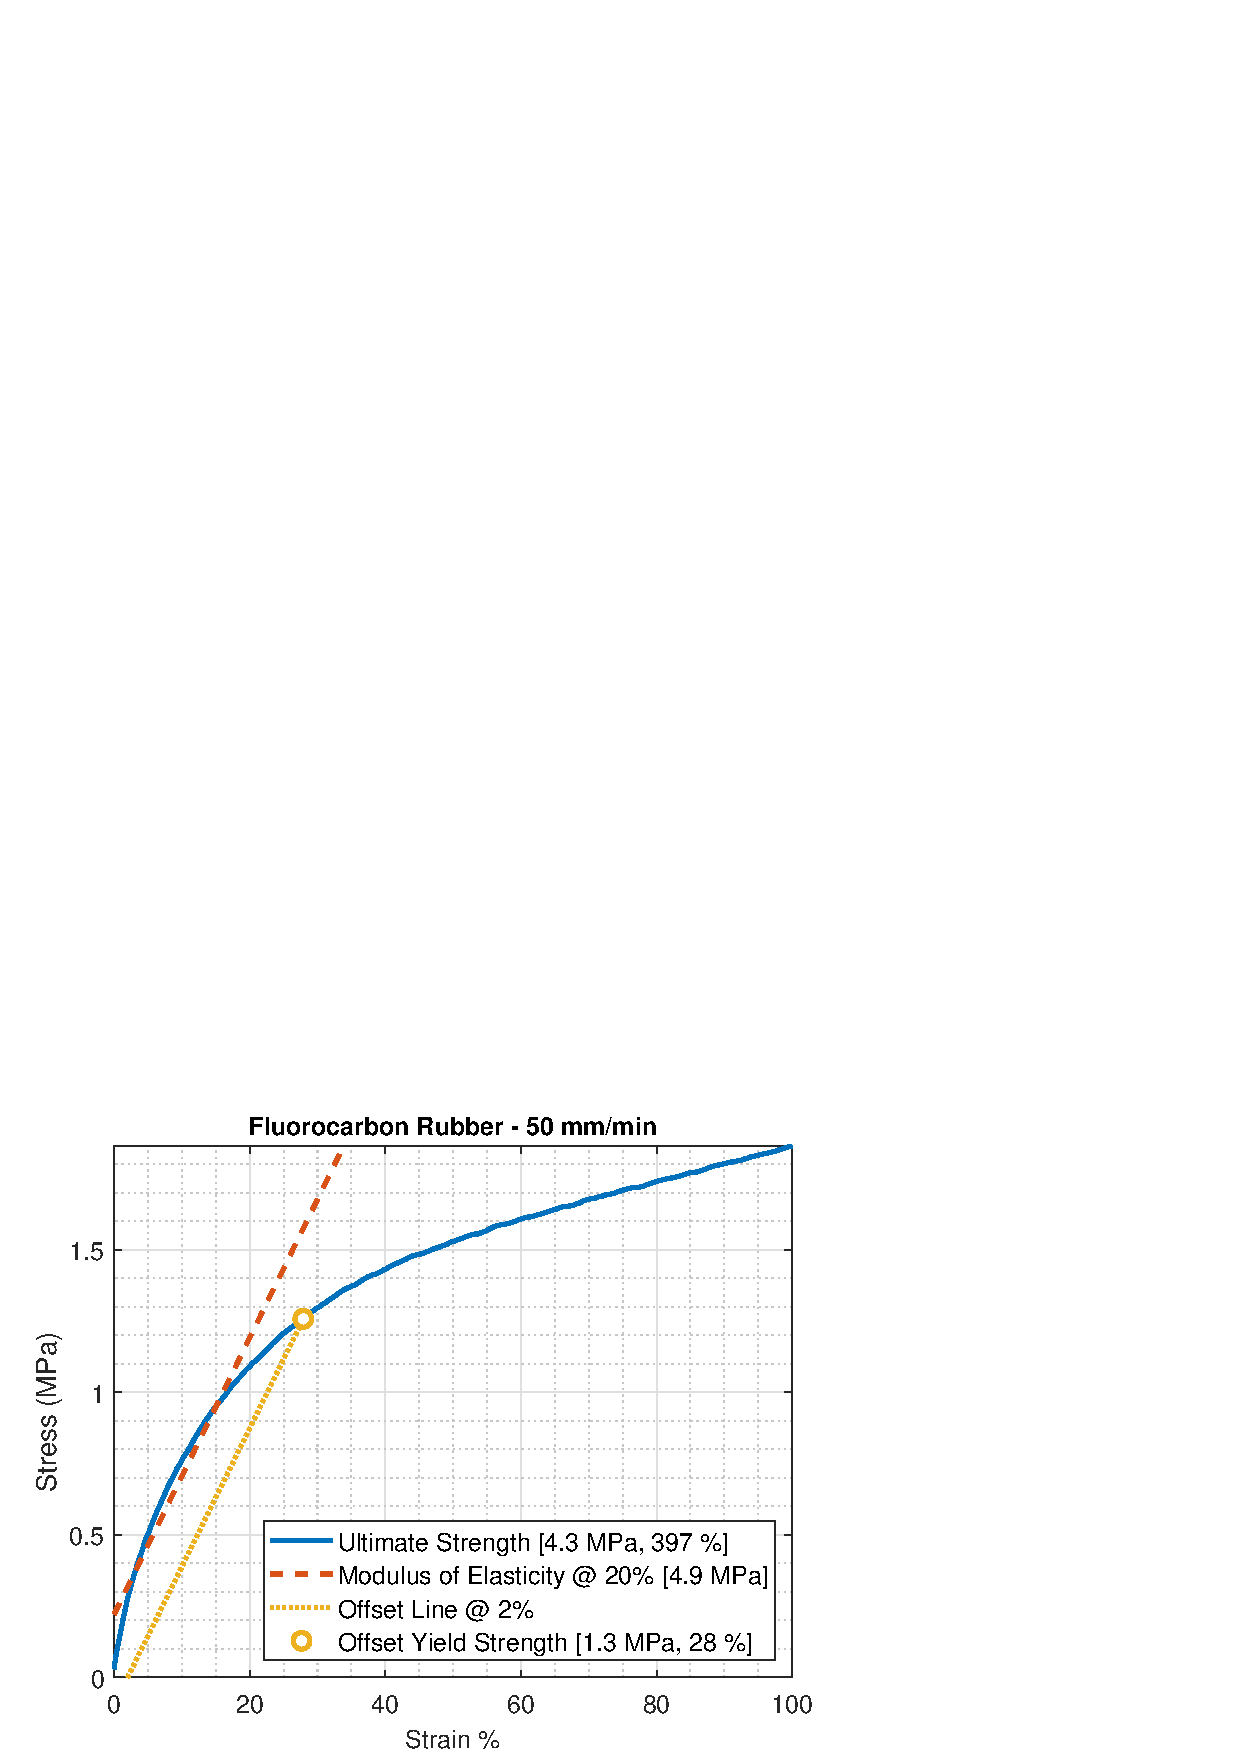
\includegraphics[width=\textwidth]{FR_disR50.png}
        \caption{}
        \label{fig:FR50}
    \end{subfigure}
    \begin{subfigure}[b]{0.65\textwidth}
        \centering
        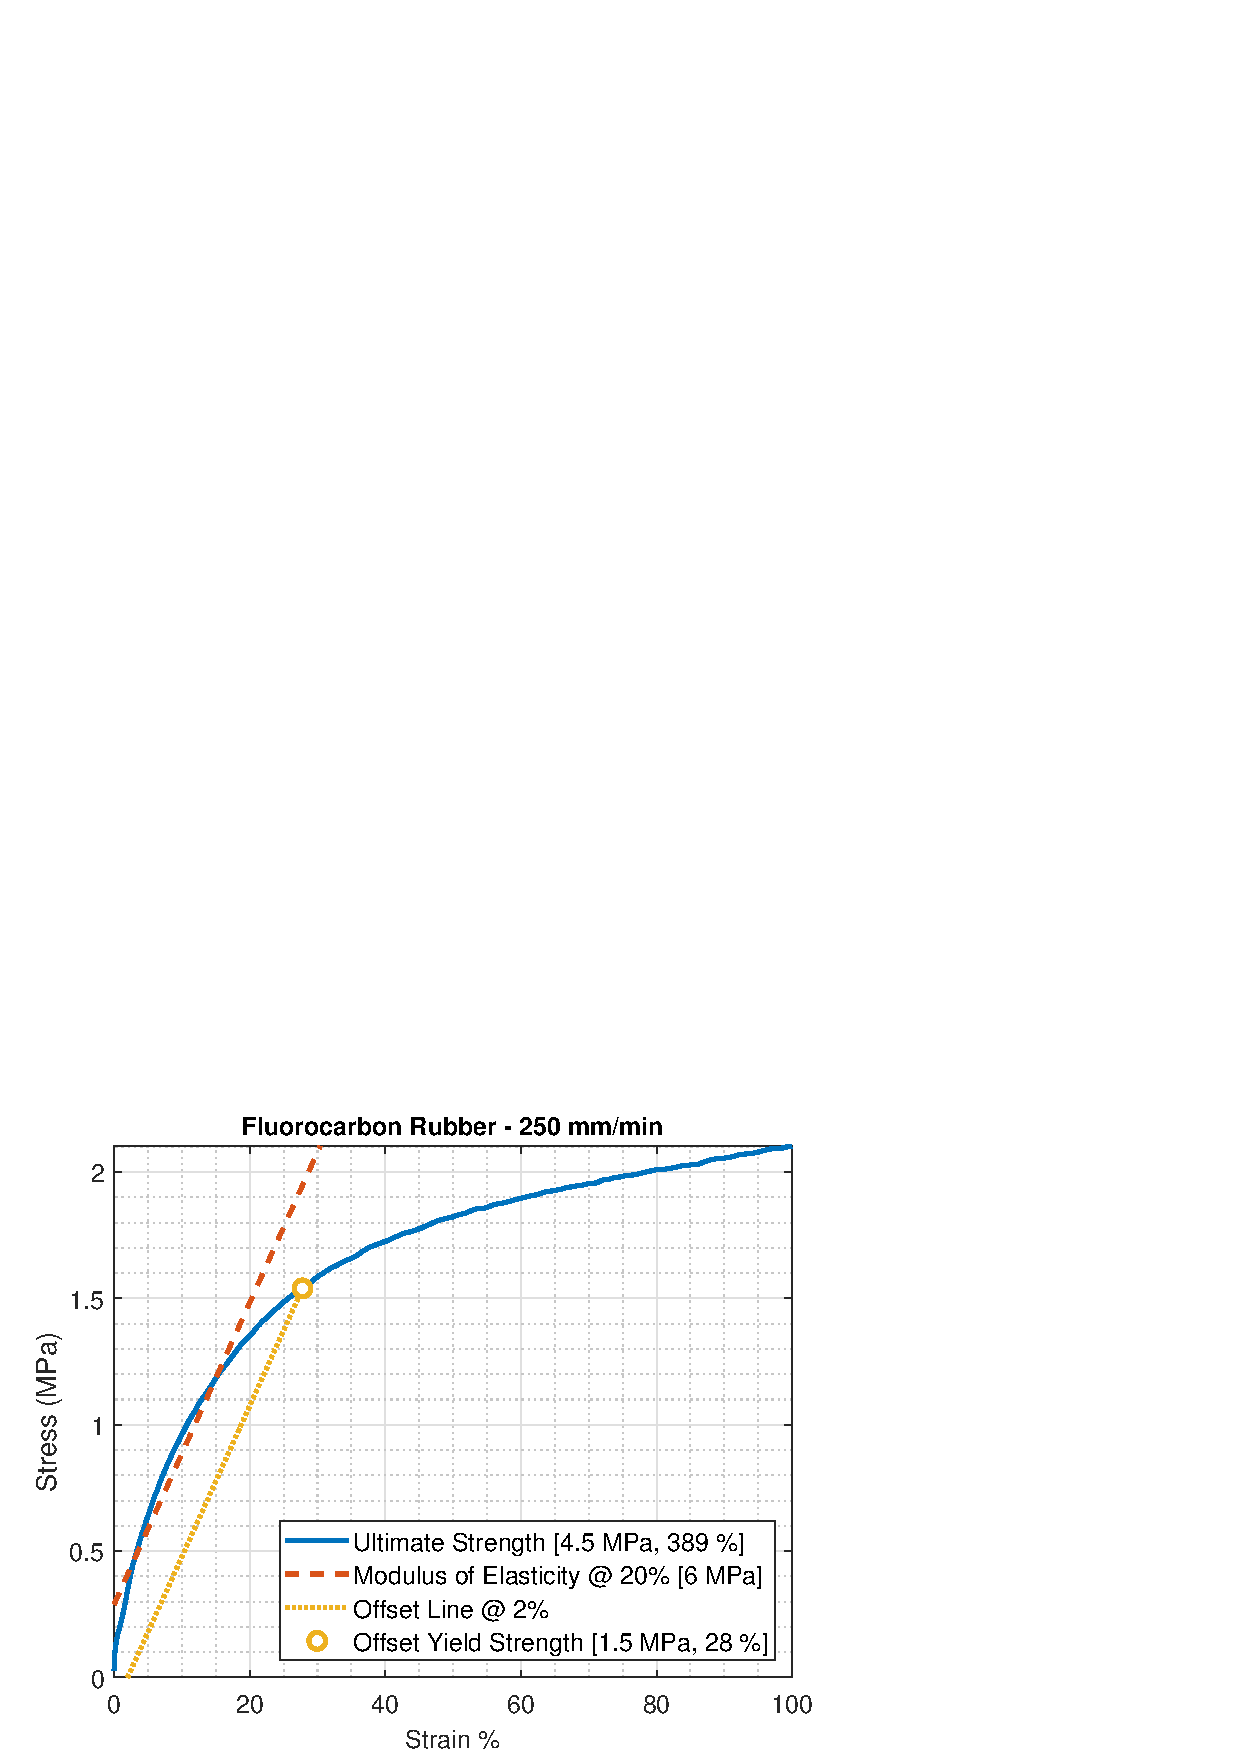
\includegraphics[width=\textwidth]{FR_disR250.png}
        \caption{}
        \label{fig:FR250}
    \end{subfigure}
    \begin{subfigure}[b]{0.65\textwidth}
        \centering
        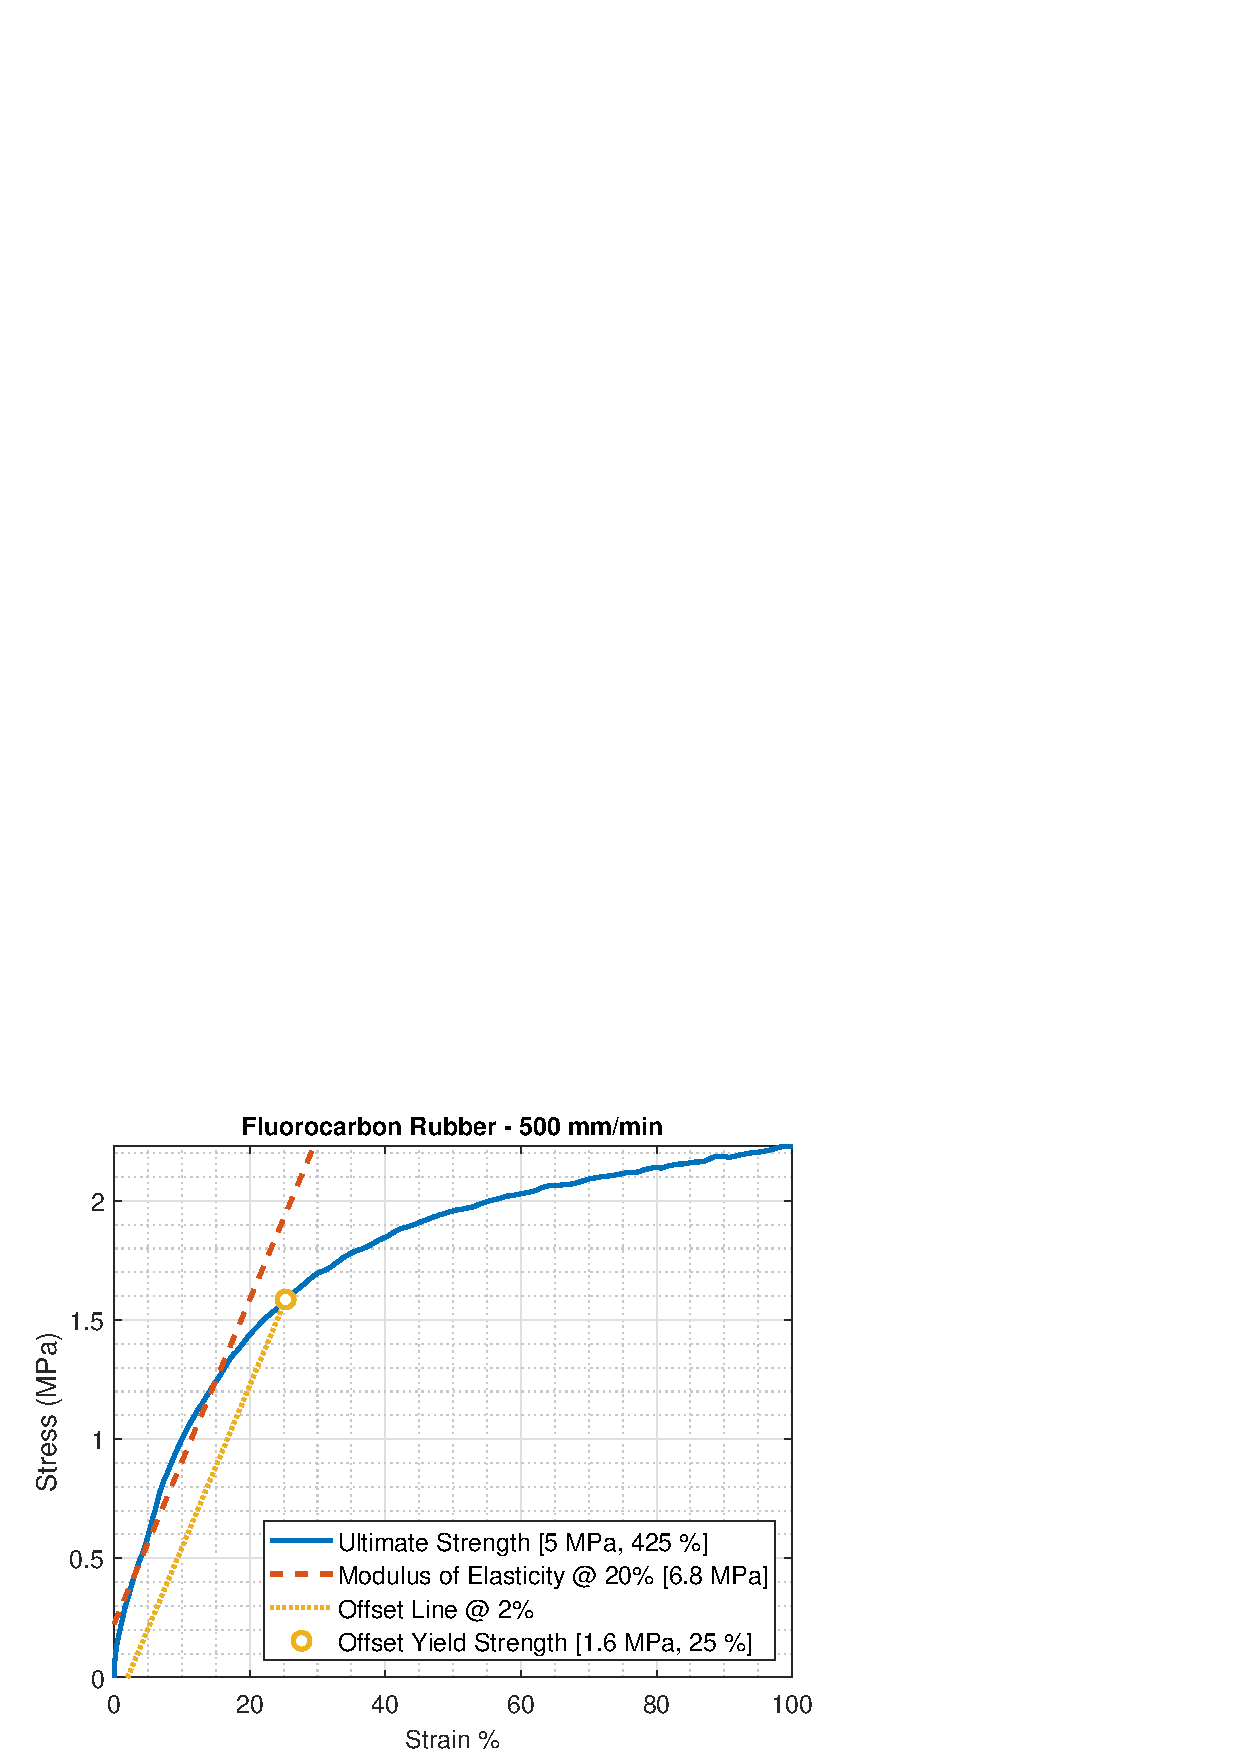
\includegraphics[width=\textwidth]{FR_disR500.png}
        \caption{}
        \label{fig:FR500}
    \end{subfigure}
    \caption{Offset Yield Strength for the FR material}
    \label{fig:FRoff}
\end{figure}
\newpage
\begin{figure}[H]
    \vspace*{-2em}
    \centering
    \begin{subfigure}[b]{0.65\textwidth}
        \centering
        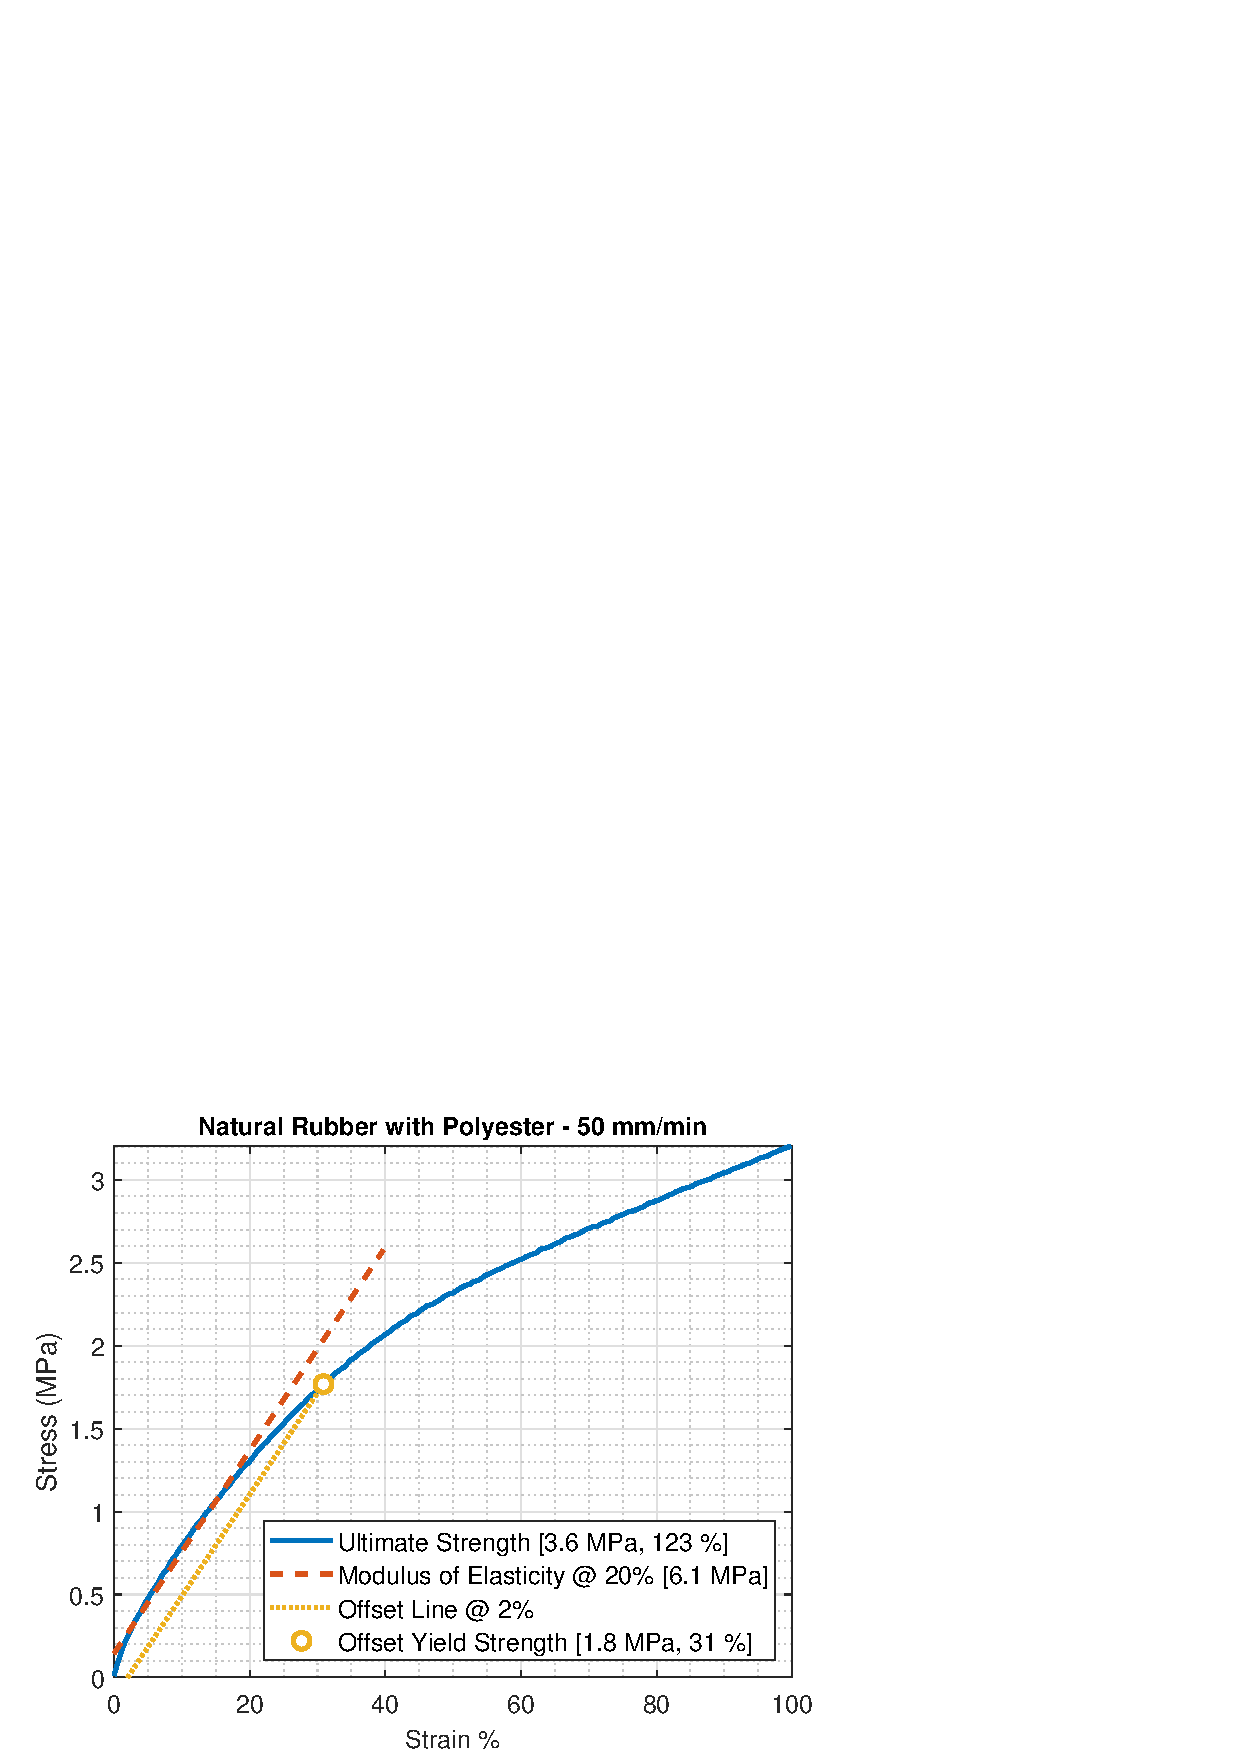
\includegraphics[width=\textwidth]{NatR_disR50.png}
        \caption{}
        \label{fig:NatR50}
    \end{subfigure}
    \begin{subfigure}[b]{0.65\textwidth}
        \centering
        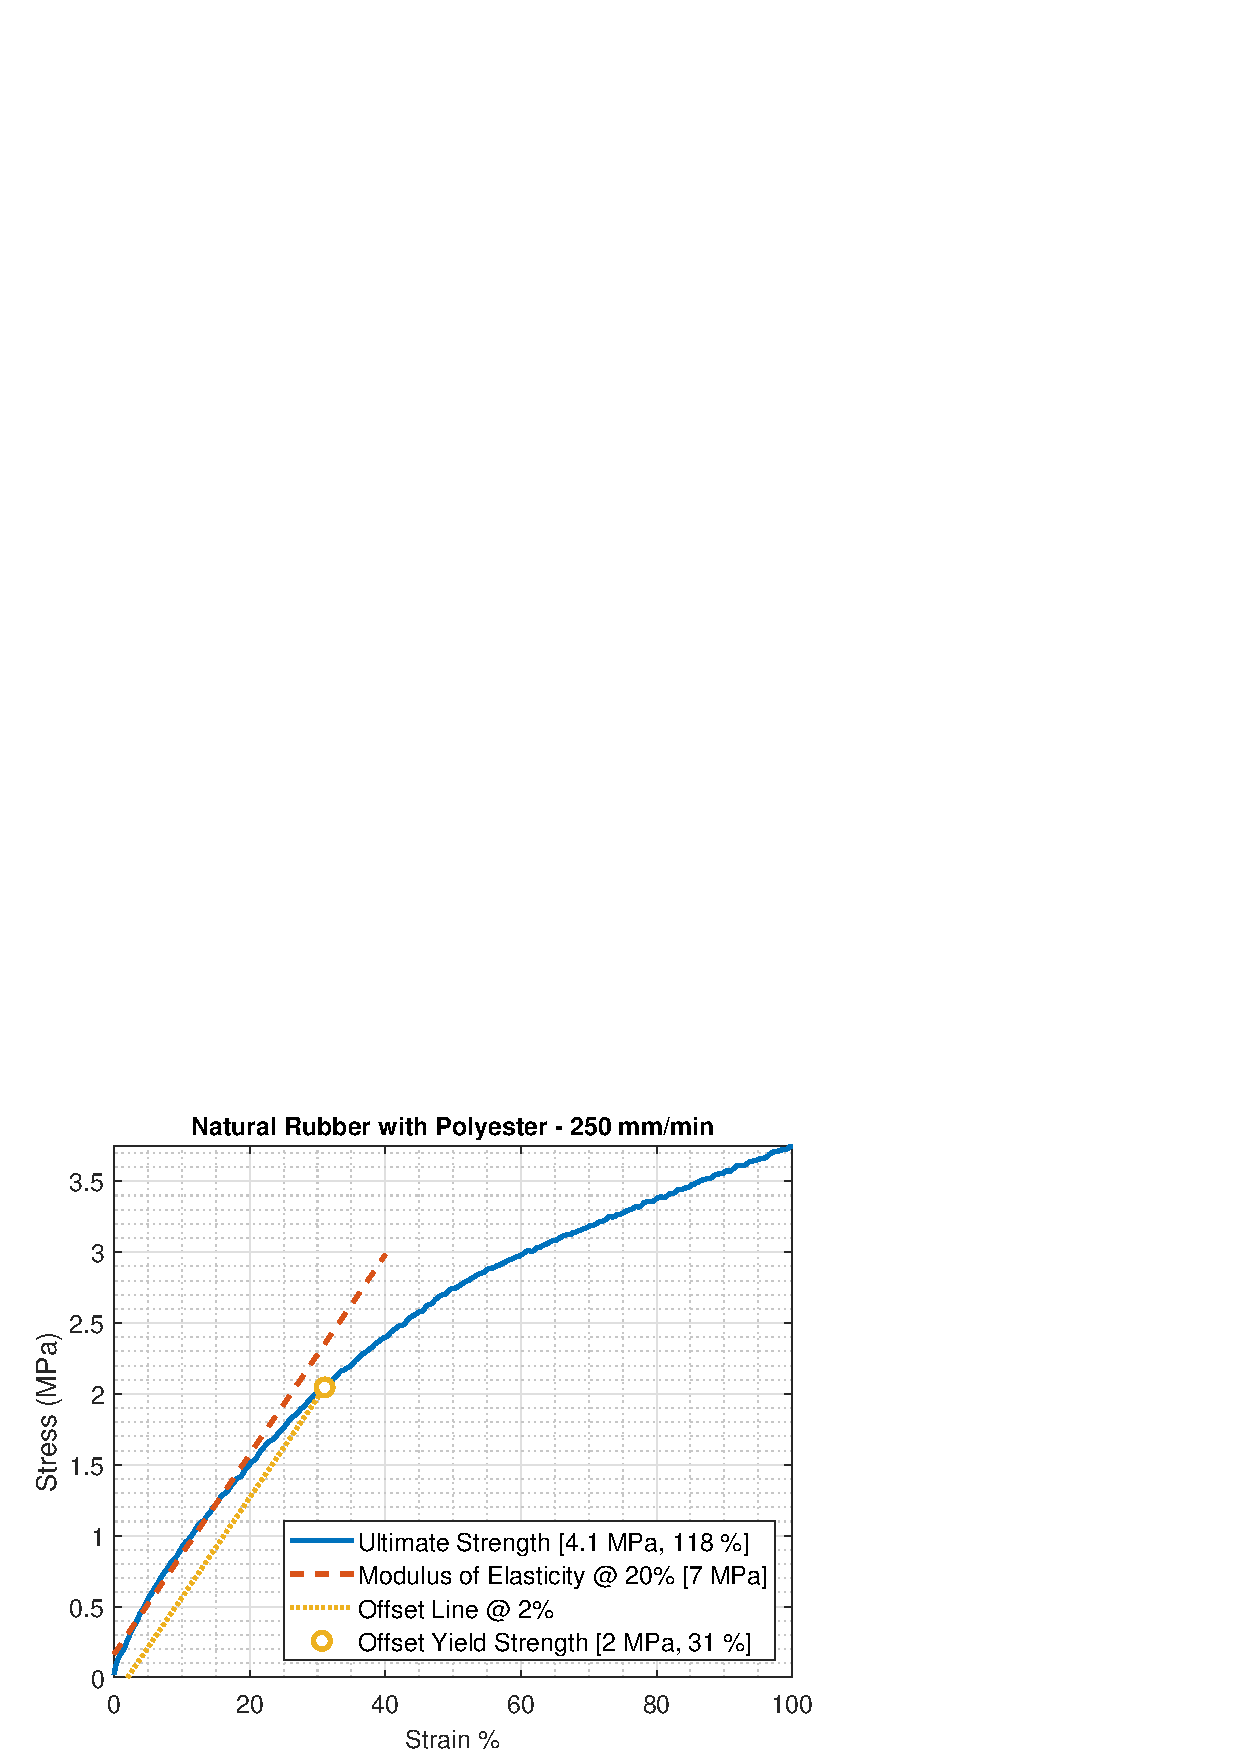
\includegraphics[width=\textwidth]{NatR_disR250.png}
        \caption{}
        \label{fig:NatR250}
    \end{subfigure}
    \begin{subfigure}[b]{0.65\textwidth}
        \centering
        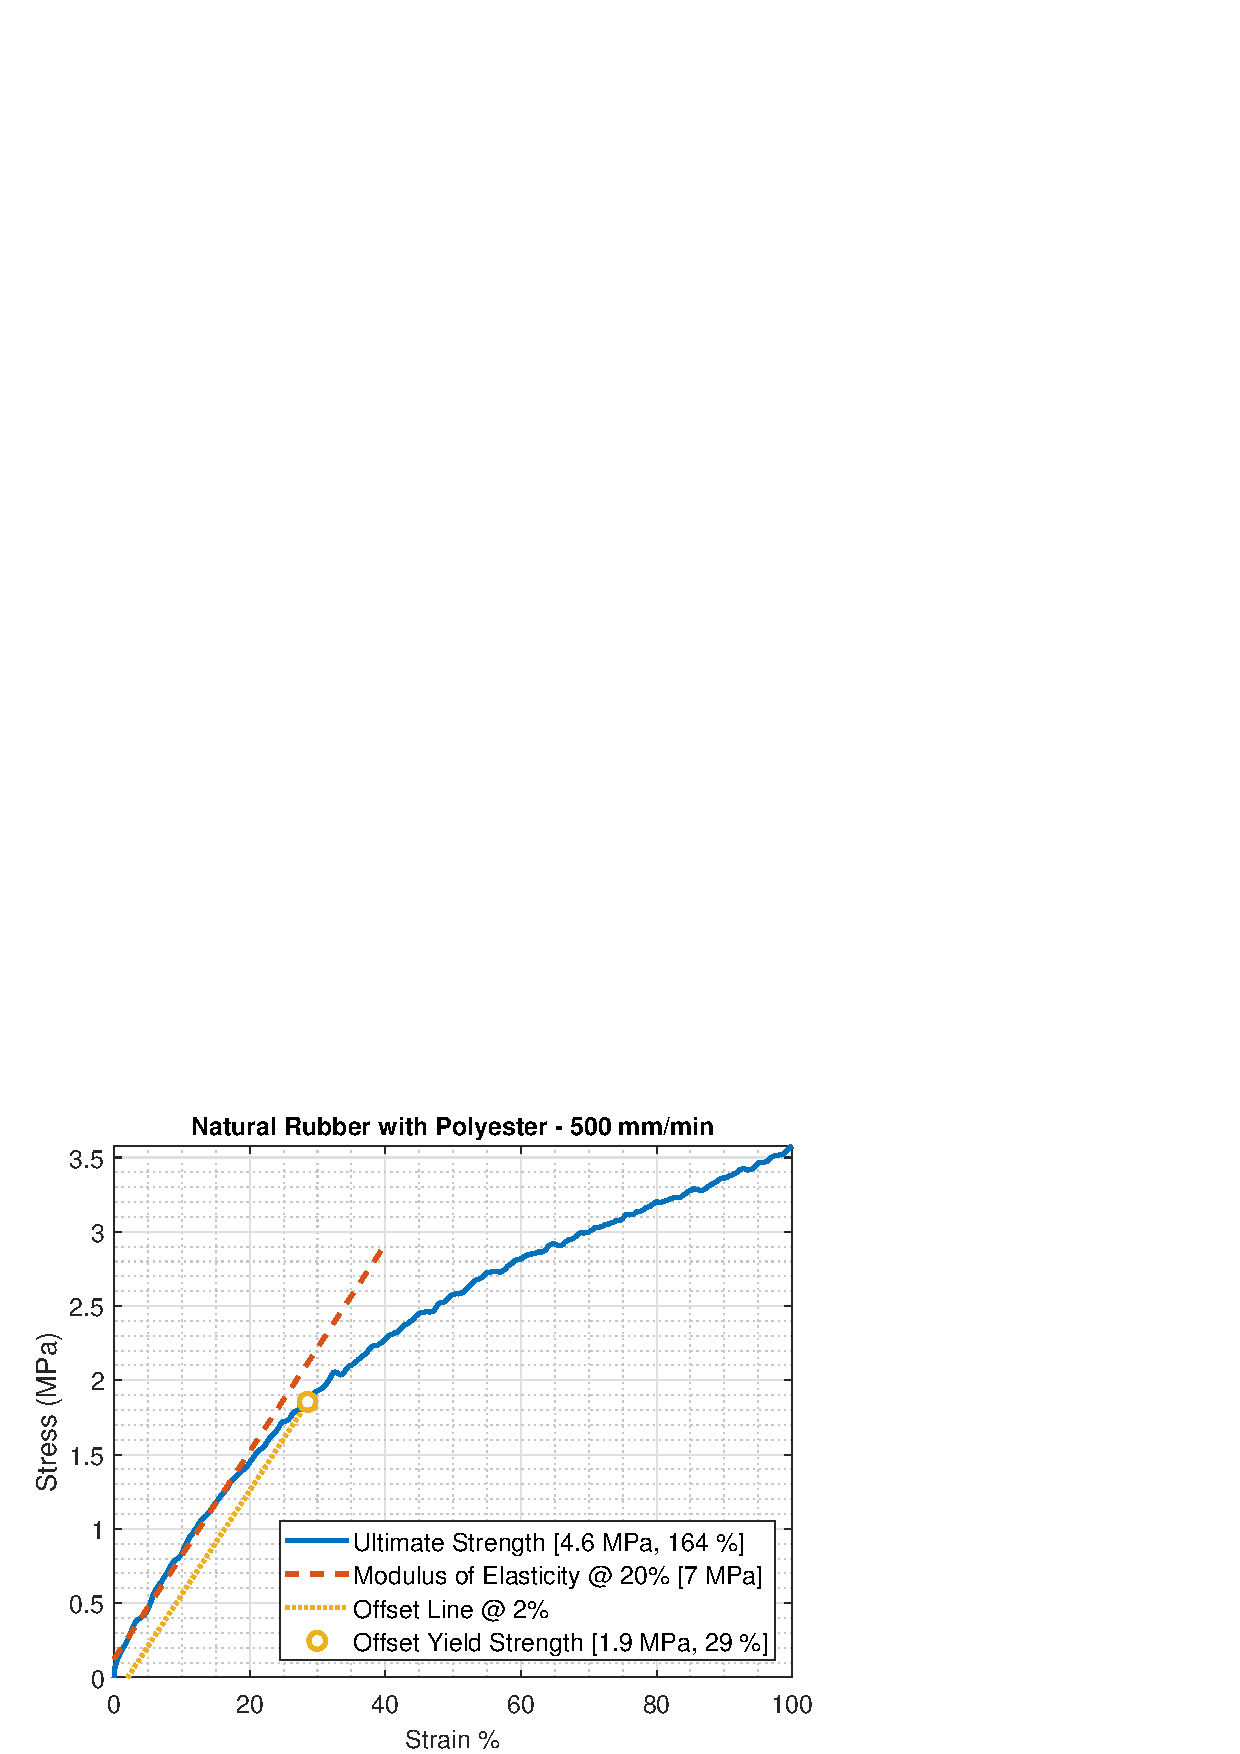
\includegraphics[width=\textwidth]{NatR_disR500.png}
        \caption{}
        \label{fig:NatR500}
    \end{subfigure}
    \caption{Offset Yield Strength for the NatPolR material}
    \label{fig:NatRoff}
\end{figure}
\newpage
\begin{figure}[H]
    \vspace*{-2em}
    \centering
    \begin{subfigure}[b]{0.65\textwidth}
        \centering
        \includegraphics[width=\textwidth]{NR_disR50.png}
        \caption{}
        \label{fig:NR50}
    \end{subfigure}
    \begin{subfigure}[b]{0.65\textwidth}
        \centering
        \includegraphics[width=\textwidth]{NR_disR250.png}
        \caption{}
        \label{fig:NR250}
    \end{subfigure}
    \begin{subfigure}[b]{0.65\textwidth}
        \centering
        \includegraphics[width=\textwidth]{NR_disR500.png}
        \caption{}
        \label{fig:NR500}
    \end{subfigure}
    \caption{Offset Yield Strength for the NR material}
    \label{fig:NRoff}
\end{figure}
\newpage
\begin{figure}[H]
    \vspace*{-2em}
    \centering
    \begin{subfigure}[b]{0.65\textwidth}
        \centering
        \includegraphics[width=\textwidth]{PR_disR50.png}
        \caption{}
        \label{fig:PR50}
    \end{subfigure}
    \begin{subfigure}[b]{0.65\textwidth}
        \centering
        \includegraphics[width=\textwidth]{PR_disR250.png}
        \caption{}
        \label{fig:PR250}
    \end{subfigure}
    \begin{subfigure}[b]{0.65\textwidth}
        \centering
        \includegraphics[width=\textwidth]{PR_disR500.png}
        \caption{}
        \label{fig:PR500}
    \end{subfigure}
    \caption{Offset Yield Strength for the PR material}
    \label{fig:PRoff}
\end{figure}
\newpage
\begin{figure}[H]
    \vspace*{-2em}
    \centering
    \begin{subfigure}[b]{0.65\textwidth}
        \centering
        \includegraphics[width=\textwidth]{Nat100R_disR50.png}
        \caption{}
        \label{fig:Nat100R50}
    \end{subfigure}
    \begin{subfigure}[b]{0.65\textwidth}
        \centering
        \includegraphics[width=\textwidth]{Nat100R_disR250.png}
        \caption{}
        \label{fig:Nat100R250}
    \end{subfigure}
    \begin{subfigure}[b]{0.65\textwidth}
        \centering
        \includegraphics[width=\textwidth]{Nat100R_disR500.png}
        \caption{}
        \label{fig:Nat100R500}
    \end{subfigure}
    \caption{Offset Yield Strength for the NatR material}
    \label{fig:Nat100Roff}
\end{figure}
\newpage
\begin{figure}[H]
    \vspace*{-2em}
    \centering
    \begin{subfigure}[b]{0.65\textwidth}
        \centering
        \includegraphics[width=\textwidth]{SR_disR50.png}
        \caption{}
        \label{fig:SR50}
    \end{subfigure}
    \begin{subfigure}[b]{0.65\textwidth}
        \centering
        \includegraphics[width=\textwidth]{SR_disR250.png}
        \caption{}
        \label{fig:SR250}
    \end{subfigure}
    \begin{subfigure}[b]{0.65\textwidth}
        \centering
        \includegraphics[width=\textwidth]{EPR_disR50.png}
        \caption{}
        \label{fig:EPR50}
    \end{subfigure}
    \caption{Offset Yield Strength for the SR and EPR (50mm/min) material.}
    \label{fig:SR-EPRoff}
\end{figure}
\begin{figure}[H]
    \vspace*{-2em}
    \centering
    \includegraphics[width=0.65\textwidth]{EPR_disR500.png}
    \caption{Offset Yield Strength for the EPR (500mm/min) material}
    \label{fig:EPR500off}
\end{figure}

In \Cref{fig:FRoff,fig:NatRoff,fig:NRoff,fig:PRoff,fig:Nat100Roff,fig:SR-EPRoff,fig:EPR500off}, the elastic region is approximated by using the offset yield strength parameter. Also, the values for the ultimate strength, yield strength, and the elastic modulus at the elastic region, are provided. Any value below the offset yield strain can be assumed to be inside the elastic region of the material, hence the material will recover its original shape after undergoing any deformation inside this range of values. Having delimited the elastic region and its elastic modulus (now $E_{small}$), the slope of the second linear portion of the curve, i.e. the elastic modulus $E_{large}$, can be approximated. Finally, the elastic properties of the material are compiled in \Cref{tbl:elasticProp}.

In \Cref{tbl:elasticProp}, the $\sigma_{ue}$ and $\varepsilon_{ue}$ are reported as the median value from the all the specimens of a specific test type. The yield values $\sigma_{y}$ and $\varepsilon_{y}$ were obtained using the offset yield strength method. The parameters $E_{small}$ and $E_{large}$ are the elastic modulus at the initial section, and middle section of the stress-strain curve. Also, $E_{small}$ is the most useful parameter for assessing the performance of a material in a real robotic application, because it describes the stiffness of a material inside the elastic region, i.e. safe working conditions. In this regards the PR material had the smallest value, whereas the NatR had the highest.

% The detailed process to calculate the offset yield strength is as follows. The first step is to apply a linear regression to the first part of the stress-strain curve. In this work, the range from 0 to 20\% strain is chosen. The slope of the fitted line represents the elastic modulus at the specified strain (20. The second step is to create a new line, starting from the specified 2\% offset strain, using the previously found elastic modulus as its slope. Finally, this line is projected up to the point in which it intersects the stress-strain curve. The stress and strain at this point represent the offset yield stress and the offset yield strain, respectively. Therefore, it is assume that beyond this point the material start undergoing plastic deformations. Similarly, it is assumed that the material is able to recover its original shape for all deformations found bellow the offset yield strain. 

\begin{table*}[htb!]
\centering
\caption{Elastic properties of the selection of soft materials.}
\label{tbl:elasticProp}
\begin{tabular}{lccccccccc} \toprule
Materials                  & Speed & $\sigma_{ue}$ & $\varepsilon_{ue}$ & $\sigma_{u}$ & $\varepsilon_{u}$ & $\sigma_{y}$ & $\varepsilon_{y}$ & $E_{small}$ & $E_{large}$ \\
                           & mm/min   & MPa &  & MPa &  & MPa &  & MPa & MPa \\
\hline
\multirow{2}{*}{EPR}      & 50    & 8.48       & 7.56       & 7.67    & 6.74    & 1.44    & 0.54    & 3.23     & 0.99      \\
                           & 500   & 9.59       & 8.84       & 9.16    & 8.41    & 1.39    & 0.51    & 4.16     & 1.1       \\
\hline
\multirow{3}{*}{FR}      & 50    & 4.36       & 3.97       & 3.96    & 3.56    & 1.5     & 0.47    & 4.83     & 0.65      \\
                           & 250   & 4.41       & 3.93       & 4.22    & 3.57    & 1.78    & 0.45    & 5.95     & 0.58      \\
                           & 500   & 5.35       & 4.29       & 4.87    & 4.07    & 1.91    & 0.45    & 6.78     & 0.61      \\
\hline
\multirow{3}{*}{NatPolR}    & 50    & 3.57       & 1.19       & 3.08    & 0.91    & 2.12    & 0.41    & 9.97     & 2.05      \\
                           & 250   & 4.06       & 1.19       & 3.91    & 1.09    & 2.51    & 0.43    & 10.74    & 2.28      \\
                           & 500   & 4.59       & 1.64       & 4.59    & 1.64    & 2.52    & 0.48    & 8.77     & 1.9       \\
\hline
\multirow{3}{*}{NR}      & 50    & 3.55       & 3.57       & 3.36    & 3.36    & 1.41    & 0.5     & 4.29     & 0.64      \\
                           & 250   & 3.65       & 3.62       & 3.58    & 3.43    & 1.47    & 0.5     & 4.63     & 0.69      \\
                           & 500   & 4.62       & 4.61       & 4.37    & 4.34    & 1.48    & 0.5     & 4.72     & 0.72      \\
\hline
\multirow{3}{*}{PR}      & 50    & 0.3        & 1.87       & 0.28    & 1.59    & 0.18    & 0.48    & 0.58     & 0.11      \\
                           & 250   & 0.33       & 1.97       & 0.31    & 1.83    & 0.19    & 0.45    & 0.66     & 0.1       \\
                           & 500   & 0.32       & 1.97       & 0.32    & 1.97    & 0.2     & 0.49    & 0.64     & 0.1       \\
\hline
\multirow{2}{*}{SR}      & 50    & 6.03       & 5.77       & 5.26    & 4.22    & 1.1     & 0.53    & 3.26     & 1.08      \\
                           & 250   & 5.68       & 4.27       & 5.52    & 4.08    & 1.15    & 0.54    & 3.26     & 1.35      \\
\hline
\multirow{3}{*}{NatR} & 50    & 9.43       & 13.02      & 9.37    & 12.93   & 0.61    & 0.69    & 1.01     & 0.33      \\
                           & 250   & 15.88      & 12.11      & 7.38    & 11.27   & 0.69    & 0.74    & 1.11     & 0.41      \\
                           & 500   & 11.93      & 12.26      & 6.61    & 11.22   & 0.73    & 0.71    & 1.19     & 0.43     \\
\bottomrule
\end{tabular}
\end{table*}


\subsection{Stress Relaxation Test}

The stress relaxation test allows the extraction of the viscoelastic properties of the materials, i.e. the time-dependent properties. In this test, a predefined and constant elongation, also called initial strain $\varepsilon_o$ is applied to the material specimen. The material is hold in place for the whole duration of the test and the stress response is recorded. The material will relax over time, i.e. the stress response will decrease. Similarly as for the tensile strength test, different combinations of test duration and initial strain values were chosen to test the materials. Also, a varying number of specimens were included in each test. Some of these combinations were based on similar characterization processes available in the literature \cite{case2015soft,delin1995volume}. As a recommendation, the value for the applied $\varepsilon_o$ must be fall beyond the elastic region of the material to avoid plastic deformation, i.e. irreparable damage. However, for highly elastic materials, such as elastomers, large values of $\varepsilon_o$ are used in the literature. Also, the material must be elongated from zero strain to the value of $\varepsilon_o$ as fast as possible. Therefore, the strain rate chosen for this test was  500 mm/min. The parameters for the performed tests are compiled in \Cref{tbl:stressRelParameters}.

\begin{table*}[htb!]
\centering
\caption{Parameters and number of collected datasets for the stress relaxation tests.}
\label{tbl:stressRelParameters}
\begin{tabular}{llccccccc} \toprule
Test & Parameters & EPR & FR & NatPolR & NR & PR & SR & NatR \\
\hline
\multirow{3}{*}{1}  & $\varepsilon_o$ (mm)      & 5 & 5 & 7 & 6 & 3 & 6 & 40 \\
                    & Duration (minutes)    & 15 & 15 & 15 & 15 & 15 & 15 & 15 \\
                    & Datasets              & 5 & 5 & 5 & 5 & 5 & 5 & 2 \\
\hline 
\multirow{3}{*}{2}  & $\varepsilon_o$ (mm)      & 20 & 10 & 6 & 5 & 4 & 15 & - \\
                    & Duration (minutes)    & 180 & 180 & 180 & 180 & 180 & 180 & 180 \\
                    & Datasets              & 1 & 1 & 1 & 1 & 1 & 1 & - \\
\bottomrule
\end{tabular}
\end{table*}

\subsubsection{Data Processing}

Similarly to the tensile strength tests, the collected data was processed prior to the extraction of the relevant parameters. The data of interest is the one found after the machine has reached the predefined $\varepsilon_o$ value. In here, several smoothing algorithms such as, moving average, Gaussian-weighted moving average, and the Savitzky-Golay algorithm, were analyzed. During testing of these algorithm, a direct relationship between the decrease in the value of the initial stress $\sigma_o$, and the selected window size, was observed. The selected window size was based on the sampling frequency and the duration of the test. The Savitzky-Golay algorithm performed better than the other two algorithms.

\subsubsection{Stress Relaxation Properties}

The stress relaxation test is useful for approximating the time relaxation constants of the materials. Commonly, viscoelastic materials have more than one relaxation constant. This is caused by the many number of internal molecular chains which relax at different rates. The stress relaxation curve of viscoelastic materials exhibit a decaying exponential stress relaxation curve. This known mathematical function, in combination with the LVMs, can be used to approximate the time relaxation constants of the material. The LVMs have the flexibility to get as complex as required by adding extra elements to the model. This latter means that the number of relaxation constants that can be extracted from the stress relaxation curve is directly proportional to the number of exponential functions contained in the LVM. This is described in detail in \Cref{sec:ModellingLVM}.

The stress at the starting and ending point of the test,  $\sigma_o$ and $\sigma_{end}$ respectively, are the minimum required parameters to approximate one relaxation constant of the material using a LVM. The achieved stress relaxation is defined by, $S.R. = 100(\sigma_o - \sigma_{end}/\sigma_o)$. Hence, the extracted properties of the materials are compiled in \Cref{tbl:stressRelProperties}. Also, the obtained stress relaxation curves of all the materials are illustrated in \Cref{fig:AllSRel,fig:PRSRel}.

\begin{table*}[htb!]
\centering
\caption{Stress relaxation properties for the selection of soft materials.}
\label{tbl:stressRelProperties}
\begin{tabular}{llccccccc} \toprule
Test & Properties & EPR & FR & NatPolR & NR & PR & SR & NatR \\
\hline
\multirow{3}{*}{1}  & $\sigma_o$ (MPa)   & 0.61      & 0.84      & 1.22      & 0.77      & 0.06      & 0.61      & 2.15 \\
                & $\sigma_{end}$ (MPa)    & 0.42      & 0.27      & 0.80      & 0.55      & 0.02      & 0.43      & 1.82 \\
                & $S.R. (\%)$    &  32     & 67      & 35      & 29      & 63      & 31      & 15 \\
                     
\hline 
\multirow{3}{*}{2}  & $\sigma_o$ (MPa)     & 1.28      & 1.13      & 1.18      & 0.72      & 0.07      & 1.11  &         \\
                & $\sigma_{end}$ (MPa)     & 0.89      & 0.41      & 0.76      & 0.55      & 0.03      & 0.80  &          \\
                & $S.R. (\%)$     & 31      & 63      & 36      & 24      & 51      & 28  &          \\
\bottomrule
\end{tabular}
\end{table*}


\begin{figure}[H]
    \centering
        \begin{subfigure}[b]{0.93\textwidth}
        \centering
        \includegraphics[width=\textwidth]{All180SRel.png}
        \caption{Caption}
        \label{sfig:ALL180SRel}
    \end{subfigure}
    \begin{subfigure}[b]{0.93\textwidth}
        \centering
        \includegraphics[width=\textwidth]{All15SRel.png}
        \caption{Caption}
        \label{sfig:centering}
    \end{subfigure}
    \caption{Caption}
    \label{fig:AllSRel}
\end{figure}

\newpage
\begin{figure}[H]
    \centering
        \begin{subfigure}[b]{0.93\textwidth}
        \centering
        \includegraphics[width=\textwidth]{PR180SRel.png}
        \caption{Caption}
        \label{sfig:PR180SRel}
    \end{subfigure}
    \begin{subfigure}[b]{0.93\textwidth}
        \centering
        \includegraphics[width=\textwidth]{PR15SRel.png}
        \caption{Caption}
        \label{sfig:PR15SRel}
    \end{subfigure}
    \caption{Caption}
    \label{fig:PRSRel}
\end{figure}

The values of $\sigma_o$ and $\sigma_{end}$ reported in \Cref{tbl:stressRelProperties}, were obtained by finding the median of the tested specimens per type of test. This is done prior to the smoothing of the data. The reported values for the achieved $S.R.$ are very similar in both tests, regarding of the duration of the test and the chosen $\varepsilon_o$. This suggest that most of the S.R. happens very early into the test. This, at the same time, could indicate that only one relaxation time constant is required to model the stress relaxation of these materials. Finally, the obtained curves are illustrated in \Cref{fig:AllSRel,fig:PRSRel}, where a quick drop in the stress response is observed at the initial portion of the curve.

%In this paragraph I could mention that depending on the linearity of the stress relaxation curve plotted in logarithmic scale, one can assume how many relaxation times are present. This part could be more suitable on the modelling chapter.

%More information on the stress relaxation modulus can be found in the Book Engineering Viscoelasticity. Although, the relevance of bringing this information in here is not clear.

\section{Summary}

In this chapter, the characterization process of the viscoelastic mechanical properties of a selection of seven different TPEs was presented. For this, the mechanical tests of tensile strength and stress relaxation was performed. In the tensile strength test, the materials were elongated until failure using up to three different strain, or elongation, rates. The latter will allow the modeling of the velocity-dependent stress response of the materials. The processing algorithm used to condition the collected data was also described in detail. The smoothing algorithm chosen for both mechanical tests was the Savitsky-Sgolay algorithm. In the case for the Natural Rubber material, where two batches were acquired, the thickness from one batch to the other varied significantly. Nevertheless, the mechanical behaviour of the material was captured accurately in the stress-strain curves. This suggest a linear proportionality between the thickness of the material and the increment on the response fore of the material. The elastic region of the materials was difficult to be identified directly due their nonlinear stress-strain curve. Therefore, the elastic region was approximated using the offset yield strength parameter. This region is very important to delimit the working conditions of the soft materials in a real robotic application. Finally, the ultimate values of strain and stress, the elastic region location, the elastic modulus in two distinctive regions of the curve, and the offset yield strength parameters, were reported. The $E_{small}$ is the most useful parameter for assessing the performance of a material in a real robotic application, because it describes the stiffness of a material inside the elastic region, i.e. safe working conditions, in contrast to the ultimate strength values. In this regards the PR material had the smallest value, whereas the NatR had the highest.

The performed stress relaxation tests can be divided in two sets. One with a low deformation, and low duration. The other, with large deformation, large duration. Regarding of this, the achieved stress relaxation of the materials was very similar for both cases. Knowing the resemblance of the stress relaxation curve with an exponential decaying function, the latter finding could suggest that only one relaxation time constant is responsible for the majority of the $S.R.$ achieved.  This hypothesis will be explored in the modeling stage. 

%Finish this chapter by: Checking Captions. Additionally, make each chapter start on an even page. Plots need to be redone
\chapter{Soft Materials Modelling: Linear Viscoelastic Models} \label{sec:ChapterModellingLVM}

%NOTE: This paper is a good literature for the next chapter about modeling, "Soft Material Characterization for Robotic Applications". In here there is a section about the variability of the materials properties from one batch to the other. However there is a consistency from specimens from the same batch

\section{Introduction}

In this chapter, the performance of two model-driven tools for the prediction of the viscoelastic properties of seven soft materials is investigated. This chapter is based on a very successful approach found in the literature, the Standard Linear model with Strain-Dependent Stiffness \cite{austin2015control}. This model make use of a piecewise linearization to improve the capabilities of one of the Linear Viscoelastic Models, the Standard Linear Solid model. Nevertheless, this approach still have some limitations which are addressed in this chapter, by performing several optimizations. Moreover, the capabilities of the latter model of accounting for velocity-dependent stress responses have not been assessed. Although, they are expected to be limited, due to the simplicity of the model.

In addition to this, the PL method is applied to a more complex model from the family of LVMs, which is the Wiechert model. This model have the advantage of accounting for velocity-dependent stress response with the trade-off of added complexity. Nevertheless, the PL method have the potential to reduce the latter complexity.

In contrast with the fitting process described in the literature \cite{austin2015control}, the stress relaxation test is used to extract the relevant parameters for the SLS and Wiechert model. Subsequently, the PL method is applied to the model, allowing them to account for strain-dependent stress responses. The performance of both models is assessed by using the stress-strain curves of six different soft materials. A seventh one is added to the last tests.

The results highlight the incompatibility between the PL method and the Wiechert model. Nevertheless, the performance of the optimized Std. Lin. SDS model is adequate. In here, the optimized version of the latter model is called PL-SLS. Similarly, the linearized version of the Wiechert model is called the PL-Wiechert model.

The relationship between the accuracy of the model and the required complexity is assessed. Furthermore, the capabilities of the PL-SLS to account for velocity-dependent stress responses is investigated. The results are mixed. On the one hand, the PL-SLS is able to generalize well the stress response, under different strain rates, of some of the studied soft materials. On the other hand, the performance of the model is found to be biased to the materials that have more dominant elastic properties. Due to this, an alternative modelling tool is proposed to be investigated in the next chapter, this time, a data-driven modelling tool.

\section{The Linear Viscoelastic Models}

As previously mentioned, soft materials have nonlinear and viscoelastic mechanical properties which cannot be easily described by mathematical models. This is a challenge faced by most of the soft robotic developments in the literature. However, the benefits using soft materials are many: energy storing, passive compliance and safe human-robot interaction. This have motivated their implementation in robotic applications and the development of mathematical models able to describe their viscoelastic properties \cite{lee2017soft}.

The human skeletal muscle system natural properties of storing and releasing energy, have motivated the inclusion of elasticity in robotic applications. Series-elastic actuators (SEAs) are the most commonly used technology. The addition of an elastic element between the actuator and the load greatly simplifies the controller design. The deformation of the elastic element can provide an indirect measurement of the applied force to the load, essentially transforming a force-control problem into a displacement-control problem \cite{agarwal2017series}. 

Traditional SEAs use metallic springs, considered as purely elastic. However, the human skeletal muscle system exhibit a viscoelastic behavior. In the literature, attempts of adding viscoelasticity to SEAs has been done by using soft materials instead of metallic springs. In fact, viscoelasticity has the potential to address many of the limitations found in series-elastic actuators, such as: low torque resolution and low bandwidth \cite{martins2015polyurethane,tagliamonte2014rendering,schepelmann2014compact}. 

The mechanical behavior of a rigid element (metallic spring) can be accurately described by known mathematical models. This is not the case for soft materials which have nonlinear and viscoelastic properties. The benefits of adding viscoelasticity to SEAs can only be fully exploited by developing a  reliable modeling tool. Substantial research has been done on this regard. However, The most accurate models are mathematically complex and computationally expensive \cite{xu2014mathematical,ciniello2017identifying,lu2017constitutive}. Nonetheless, even these complex models cannot account for all the different  factors which modify the materials properties, such as the manufacturing process and internal weakening of the material after being loaded for the first time \cite{case2015soft}. The latter highlights the difficulty of developing mathematical models which account for both microscopic and macroscopic aspects of the materials. This has motivated researchers to implement alternative methods for characterizing a material, such as Finite Element Analysis (FEA).

In robotics applications, where the controller can compensate the lack of accuracy in describing the controlled plant, a simple and fairly accurate model is preferred over a very accurate and highly complex one. For this reason, a known set of mathematical models, the Linear Viscoelastic Models (LVMs) are commonly used for the prediction of viscoelasticity in soft materials. In contrast to the mechanical model for Hooke's Law, which is based on a single spring, the LVMs are based on two fundamental mechanical components, a spring and a dashpot, which can be arranged in different configurations and quantities. This is illustrated in (\Cref{fig:LinearViscoelasticModels}).

\begin{figure}[hbt!]
	\centering
    \includegraphics[width=0.6\textwidth]{HookeViscoelasticModels.PNG}
    \caption{Hooke's Law and linear viscoelastic models: (a) Hooke's Law (b) Kelvin-Voigt, (c) Maxwell, (d) Standard Linear Solid, and (e) Burger. The parameters $k$ and $\eta$ represent the spring stiffness and the dashpot viscous constant, respectively \cite{austin2015control}. }
    \label{fig:LinearViscoelasticModels}
\end{figure}

In line with the mentioned approach of relying on the controller to compensate the limitations of simple models, the work performed by Austin et al. modifies the viscoelastic Standard Linear Solid (SLS) model by implementing a piecewise linearization (PL) \cite{austin2015control}. The authors chose this model instead of the more complete, hence more complex, Burger model to keep the modeling process as simple as possible. The implementation of the PL method allowed the SLS model to account for the nonlinear properties of the material stress response. Due to this, the developed model is called the Standard Linear Solid model with Strain-Dependent Stiffness (Std. Lin. SDS). Nevertheless, the developed model was still unable to account for the material hysteresis, and, due to hardware limitations, the velocity-dependent stiffness effects were not validated. Moreover, experimental tests validated the changes on the material stiffness depending on the velocity of the applied deformation.

The PL method have proven to be a successful way to improve the prediction ability of traditional LVMs. Although it still has some limitations. The latter is addressed in this chapter by implementing the PL method in a more complex member of the LVMs, the Wiechert model. This is described in detail in \Cref{sec:wiechert}.

\section{The piecewise linearization method on the Wiechert model} \label{sec:wiechert}

The SLS model is frequently used when modeling viscoelastic materials, mainly due to its fairly simple mathematical model and its ability to account for creep and stress relaxation of the material (time-dependent properties). The SLS model can be viewed as a Maxwell model (also known as Maxwell branch) with an extra spring connected in parallel. The simplicity of the SLS model is also its main limitation. 
Viscoelastic materials are known to have more than one relaxation time, i.e. more than one Maxwell branch. In the linear viscoelastic models, the relaxation time depends on the viscous elements, i.e. dashpots. The Wiechert model, which is essentially a SLS model with $j$ Maxwell branches, is able to account for $j$ relaxation times and is illustrated in \Cref{fig:wiechert}. The time-dependent behavior of any viscoelastic material can be fully described by this model, given enough numbers of elements. However, the complexity of the model increases in proportion to the number of extra branches. Mathematically, each extra branch increases the derivative order of the model since more equations are required to account for the extra variables \cite{tirella2014strain,roylance2001engineering}.

\begin{figure}[hbt!]
	\centering
    \includegraphics[width=0.3\textwidth]{WiechertModel.png}
    \caption{Wiechert Model. The components $k_1$, $\eta_1$, and the equilibrium spring $k_e$, together represents the SLS model. The components $k_j$, and $\eta_j$ represents the Maxwell Branch. The Wiechert model can contain as many branches as required, this is symbolised by the subscrip $j$. }
    \label{fig:wiechert}
\end{figure}

As previously described in \Cref{sec:viscoelasticity}, in addition to time-dependent and history-dependent properties, elastomers also have a nonlinear stress response. This can be partially described by the LVMs. The relaxation time constant of the dashpots in these models describes the nonlinear but time-dependent stress response of the material. Nonetheless, LVMs are not able to account for the strain-dependent response of materials. The latter is solved by the PL method as described in \cite{austin2015control}.

The spring in parallel with the other elements, in both the SLS model and the Wiechert model, is known as the equilibrium spring, and its stiffness $k_e$, is assumed constant. In reality, the stiffness $k_e$ of most elastomers is strain-dependent. 

Early attempts of modeling a strain-dependent stress response in viscoelastic materials are described by Schepelmann et al. in \cite{schepelmann2014compact}, where the stress-strain curve of a nonlinear rubber spring is approximated with an exponential model. In subsequent works, Austin et al. describes a piecewise linear regression fitted to the stress-strain curve of a material, in combination with the SLS model. 

The slope of the stress-strain curve represents the material's Young Modulus which is proportional to the material stiffness. During a tensile strength test the material is deformed at a constant rate, i.e. the stress response of the viscous element is also constant. Therefore, the observed nonlinear response is caused by the equilibrium spring.

Using the PL method, the nonlinear behavior of the equilibrium spring is approximated by considering it as several springs in parallel which ``engages" in sequence as the material strain increases. This is modeled by a summation of Heaviside functions centered in the desired strain in which each of the mentioned springs ``engages" and contributes with the total stress response of the material. In other words, the stress-strain curve of the material is segmented in several sections which relates a single stiffness to a strain range. This is illustrated in \Cref{fig:PLmethod}.

\begin{figure}[htb!]
	\centering
    \includegraphics[width=0.6\textwidth]{PLmethod.png}
    \caption{(a) Standard Linearized Solid model with Strain-Dependent Stiffness. (b) Piecewise linearization method applied to the slope of the material load-displacement curve. This is analogous to many parallel springs which contribute to the material response depending on the material strain \cite{austin2015control}}.
    \label{fig:PLmethod}
\end{figure}

\subsection{Model fitting} \label{sec:Modelfit}

The mathematical expression for the SLS model and the Wiechert model can be simplified when considering a constant strain input (stress relaxation test). This simplification allows these models to be fitted into the stress relaxation curve and to approximate the parameter of interest, $k$ and $\eta$ \cite{roylance2001engineering}. The mathematical expression for the Wiechert model under a constant strain input is given by:

\begin{equation}
\label{eq1}
\sigma(t)=\Bigg\{k_e +  \sum_{j} k_j e^{-t/\tau_j}\Bigg\}\epsilon_o
\end{equation}

\noindent where $\sigma$ is the stress at a given time, $k_e$ is the equilibrium spring stiffness and $\varepsilon_o$ is the initial strain. For the summation, $\tau_j=\eta_j/k_j$ is the relaxation time constant, $k_j$ and $\eta_j$ are the spring stiffness and viscous constant of the elements in the $j^{th}$ Maxwell branch, respectively. For the specific case when $j = 1$, the resulting equation describes the SLS model under a constant strain input. In this case, the three parameters described in the SLS model: equilibrium spring stiffness $k_e$, dashpot viscous constant $\eta$ and the spring stiffness in the Maxwell branch $k_1$, can be obtained from the stress relaxation curve by analyzing three significant points: $t=0$, $t=\tau$, and $t=\infty$, as illustrated in \Cref{fig:stressTimeCurve}. The longer the duration of the test, the better the approximation of $k_e$.

\begin{figure}[htb!]
	\centering
    \includegraphics[width=0.6\textwidth]{StressTimeCurve.png}
    \caption{SLS model fitted to a typical stress relaxation curve of a viscoelastic material. The parameters $k_e$, $k_1$ and $\eta$ can be obtained by analyzing three points in the curve: $t=0$, $t=\tau$, and $t=\infty$.}
    \label{fig:stressTimeCurve}
\end{figure}

The process to extract the parameters of the Wiechert model is more complicated due to its extra Maxwell branches, i.e. there are more than three points in time to be analyzed. These points can be selected using a collocation technique \cite{roylance2001engineering,machiraju2006viscoelastic}. In the reviewed literature, the points of interest are linearly scattered throughout the whole duration of the stress relaxation curve. Nevertheless, the decaying exponential term in \Cref{eq1} is better approximated by selecting the points of interest using a logarithmic scale. This is possible with the MATLAB function \texttt{logspace} which spreads evenly the desired number of points between the allowable decades. 
This is better described with the following example. A Wiechert model with six branches, $j=6$, wants to be fitted into a stress relaxation curve with four decades of duration ($t=10^4$ seconds). In total it would be required seven points in time, one for each branch and one for $t=0$. These points are spread as evenly as possible, using the total duration of the test, by the function \texttt{logspace}. The point $t=0$ is required for a correction described in the following paragraph. 

Similarly to the process illustrated in \Cref{fig:stressTimeCurve}, each point in time represents a time constant $\tau_j$ for which there is a known stress $\sigma_j$ from the experimental data. This can be rearranged into an equation system of $j$ equations with $k_j$ as the unknown variable as described in \cite{machiraju2006viscoelastic}. 

%Maybe bring the system of equations here?

Prior to this step, $k_e$ can be obtained using the equation for $\sigma(\infty)=\varepsilon_o k_e$, as illustrated in \Cref{fig:stressTimeCurve}. Subsequently, The Wiechert model in \Cref{eq1} can be completely described by solving the mentioned system of equations. Finally, after obtaining all the $k_j$, the value of $k_1$ is corrected, as described in \cite{roylance2001engineering}, by analyzing the point in time $t=0$.

The previous process allows the wiechert model equation to be fitted into the stress relaxation curve for a defined number of branches $j$. However, to obtain the optimal number of branches for each material, an iterative algorithm to find the smallest root mean square error (RMSE) between the Wiechert model response and the experimental data after testing different number of branches in the range of $j=[1,10]$ is implemented. The obtained optimal number of branches for each material varied between the range $j=[8,10]$. A higher number of branches has a meaningless improvement on the RMSE. Furthermore, beyond the number of branches $j=20$ the Wiechert model response shows an oscillatory behavior, hence a higher RMSE. Having obtained the parameters of interest for the SLS and the Wiechert model, their stress response under a constant strain is compared against the experimental data in Fig. \Cref{fig:StressRelFit}. 

\Cref{fig:StressRelFit} highlights the better accuracy delivered by the extra Maxwell branches in the Wiechert model in comparison to the simpler SLS model. As previously mentioned, \Cref{eq1} is a simplification helpful to approximate the parameters of both models but it is only applicable when the strain input is constant. The mathematical expression for the Wiechert model which describes the stress response under an unknown strain input, also called the constitutive equation can be found in \cite{roylance2001engineering}, in its Laplace. 
As previously mentioned, the Wichert model is an extension of the SLS model. Hence, when making $j=1$, the constitutive equation of the SLS model can be obtained, i.e. for an unkown strain input, is presented as follows:

\begin{figure}[htb!]
	\centering
    \includegraphics[width=0.93\textwidth]{SRelFit.png}
    \caption{Obtained fit from the Standard Linear Solid (SLS) and Wiechert model on the stress relaxation curve of the Silicone Rubber material. The obtained optimal number of branches of the Wiechert model fit is $j=8$.}
    \label{fig:StressRelFit}
\end{figure}

\begin{equation}
\label{eq3}
\dot{\sigma} + \frac{\sigma}{\tau_1} =  (k_e + k_1)\dot{\epsilon} + \frac{k_e\epsilon}{\tau_1}
\end{equation}

\noindent where $\epsilon$, $\dot{\epsilon}$, and $\dot{\sigma}$ are the strain, the strain rate and the stress rate, respectively (for the detailed procedure refer to \cite{roylance2001engineering}). Notice that the previous procedure will yield into a higher derivative order equation when applied to the Wiechert model due to its extra branches. A higher number of branches will increase the model accuracy at the cost of increasing its mathematical complexity. The constitutive equation of a Wiechert model with $j$ branches would result in a $j$ order differential equation similar to \Cref{eq3}. The aim of this chapter s to apply the PL method to the Wiechert model and evaluate its performance. Therefore, solving dealing with differential equations is out of the scope. Nonetheless, the Wiechert model can be evaluated by transforming it into a finite differences equation, as explained in \cite{roylance2001engineering}, yielding the following equation:

\begin{equation}
    \label{eq4}
    \sigma^t = k_e\epsilon^t + \sum_j \frac{k_j(\epsilon^t - \epsilon^{t-1}) + \sigma_j^{t-1}}{\bigg(1+\dfrac{\Delta t}{\tau_j}\bigg)}
\end{equation}

\noindent where the superscript $t-1$ and $t$ refers to values before and after a small time step $\Delta t$ have passed. Once again, making $j=1$ on \Cref{eq4} yields the finite difference version of the SLS model. The response of the two viscoelastic models of interest will be compared against the experimental data from the tensile strength test.

The next step in the fitting process focuses on the tensile strength test. In this test, the strain rate is constant, hence the resulting stress for both models (Fig. \Cref{fig:LinearViscoelasticModels}) is dependent on both the equilibrium spring and the Maxwell branches. At this stage of the model fitting, the parameters of the Maxwell branches in both models are known and their stress response can be calculated. The stress response of the equilibrium spring, $k_e$, can be isolated by subtracting the stress response of the Maxwell branches to the stress measured in the tensile strength test. 

After isolating the stress response of $k_e$, the final step in the fitting process is to implement the PL to both models and compare their response against the experimental data. Firstly, the stress-strain curve from tensile strength test is divided into $n$ segments. As previously explained, $k_e$ is considered as a group of parallel springs which ``engage" as the strain increases. This means, each subsequent stiffness is a combination of the ones found in previous segments of the stress-strain curve (Fig. \Cref{fig:PLmethod}).  Lastly, a linear regression is applied on the stress-strain curve for the desired $n$ strain segments to find the slope of the curve. This slope represents the stiffness of the equilibrium spring in each segment. By combining the $n$ obtained stiffness, the stress response of the strain-dependent stiffness $k_i^*$ is defined as follows:

\begin{equation}
\label{eq5}
\sigma^* = \sum_i^n k_i^* H_{\epsilon - \epsilon_i}(\epsilon - \epsilon_i)
\end{equation}

\noindent where $n$ is the desired number of strain intervals to fit, $\varepsilon_i$ represents the strain value at which the $i^{th}$ spring starts contributing to the stress response, the $H_{\epsilon - \epsilon_i}$ is the Heaviside or unitary step function centered at $\varepsilon_i$, i.e. the function output goes from 0 to 1 when $\varepsilon - \varepsilon_i = 0$. By substituting \Cref{eq5} into \Cref{eq3}, the Standard Linear Solid model with Strain-Dependent Stiffness is obtained \cite{austin2015control}.

Linear viscoelastic models describe a nonlinear relationship (decaying exponential time relaxation) between the applied strain and the resulting stress in a material. However, they only account for a linear stress response of the equilibrium spring. In reality, the relocation of internal molecular chains causes viscoelastic materials to exhibit a nonlinear and strain-dependent stress response. This can be solved by implementing the PL into \Cref{eq4}. The equilibrium spring stiffness $k_e$ is replaced by the strain-dependent stiffness $k_i^*$, yielding the linearized Wiechert model (PL-Wiechert) in \Cref{eq6}. Subsequently, the Std. Lin. SDS model, found in \cite{austin2015control}, is transformed into a finite difference equation, yielding \Cref{eq7}.

\begin{equation}
\label{eq6}
\sigma^t = \sigma^* + \sum_j \frac{k_j (\epsilon^t-\epsilon^{t-1}) + \sigma_j^{t-1}}{\bigg(1 + \dfrac{\Delta t}{\tau_j}\bigg)}
\end{equation}

\begin{equation}
\label{eq7}
\sigma^ t = \frac{1}{\bigg(1+\dfrac{\Delta t} {\tau_1} \bigg)} \Bigg[ \frac{\Delta t}{\tau_1} \sigma^* + (\sigma^* + k_1) (\epsilon^t-\epsilon^{t-1}) + \sigma^{t-1} \Bigg] 
\end{equation}

In this chapter, the linearized SLS model (\Cref{eq7}) is labelled as the piecewise linearized SLS (PL-SLS) model, differentiating it from the Std. Lin. SDS model documented in \cite{austin2015control} because the implemented fitting process is different. In here, the additional step of removing the stress response of Maxwell branches is performed. In summary, the experimental data from the stress relaxation test was used to obtain the parameters in the Maxwell branches of both models. The required number of branches was different per material, ranging from $j=8$ to $j=10$.  The constitutive equation of the Wiechert model was expressed as an equation of finite differences and subsequently linearized to obtain \Cref{eq6} (PL-Wiechert). Similarly, the constitutive equation of the SLS model, \Cref{eq3}, was modified in the same way, yielding \Cref{eq7} (PL-SLS).

\subsection{Findings}

At this stage of the research only six out of the seven soft materials previously mentioned were studied. The material missing in the following analyses is the Natural Rubber. Moreover, the stress-strain curves from the materials studied in this section are from the tensile strength test with 500 mm/min strain rate. With the exception of the Silicon Rubber material, for which the stress-strain curve for a strain rate of 50 mm/min was used. The complete list of the different tensile strength tests performed per material can be found in \Cref{tbl:tensile_tests}.

\subsubsection{Analysis of the optimal number of strain segments}

The amount of strain segments and their proper collocation have an impact on the PL method accuracy. In the work presented by Austin et al. there is no explanation of the criteria used to select the strain segments, only an illustration is provided \cite{austin2015control}. In this work, the variation of the slope in the stress-strain curve was used as the selection criteria. An optimization algorithm, which automatically collocates a new strain segment when the slope has varied outside a defined tolerance boundary, was developed.

The benefit of using this tolerance as the selection criteria for the number of strain segments to be created by the PL method, is two folds. On the one hand, the relationship between the number of strain segments and the desired tolerance is found to be exponential. On the other hand, the achievable RMSE for both models, in general for all materials, have minimal changes above a certain number of strain segments. In other words, beyond a certain number of strain segments, small improvements in the model accuracy requires a very large number of strain segments. This highlights a design trade-off between good accuracy and high computational complexity.

The PL-SLS model benefits the most from the PL method. It delivers a good accuracy even for small number of strain segments (\Cref{fig:SegmentsAll}). In contrast, the accuracy of the PL-Wiechert does not improve when using higher numbers of strain segments. Moreover, in the cases for the SR and EPR materials, the accuracy gets worse as the number of strain segments increases (\Cref{fig:SegmentsSR} and \Cref{fig:SegmentsEPR}).

The charts in \Cref{fig:SegmentsAll} are useful to select a proper value for the slope variation tolerance, taking into account the previously mentioned trade-off. It can be appreciated that the optimal tolerance is different for each material and dependent on the application. For the sake of analyzing the effect of the number of strain segments in the stress response of the PL-SLS and the PL-Wiechert models the tolerance value of 20\% is chosen. The obtained fit of both models is compared against the experimental data on \Cref{fig:ResponseAll}.

\begin{figure}[htb!]
    \centering
    \begin{subfigure}[b]{0.49\textwidth}
        \centering
        \includegraphics[width=\textwidth]{Segments_SR.png}
        \caption{}
        \label{fig:SegmentsSR}
    \end{subfigure}
    \begin{subfigure}[b]{0.49\textwidth}
        \centering
        \includegraphics[width=\textwidth]{Segments_EPR.png}
        \caption{}
        \label{fig:SegmentsEPR}
    \end{subfigure}
    \begin{subfigure}[b]{0.49\textwidth}
        \centering
        \includegraphics[width=\textwidth]{Segments_FR.png}
        \caption{}
        \label{fig:SegmentsFR}
    \end{subfigure}
    \begin{subfigure}[b]{0.49\textwidth}
        \centering
        \includegraphics[width=\textwidth]{Segments_NR.png}
        \caption{}
        \label{fig:SegmentsNR}
    \end{subfigure}
    \begin{subfigure}[b]{0.49\textwidth}
        \centering
        \includegraphics[width=\textwidth]{Segments_NatR.png}
        \caption{}
        \label{fig:SegmentsNatR}
    \end{subfigure}
    \begin{subfigure}[b]{0.49\textwidth}
        \centering
        \includegraphics[width=\textwidth]{Segments_PR.png}
        \caption{}
        \label{fig:SegmentsPR}
    \end{subfigure}
    \caption{Relationship of the desired tolerance between the number of strain segments (blue bars), and the achievable rRMSE of the PL-SLS (solid red) and the PL- Wiechert (solid green) models, for all the soft materials (a-f). Figure taken from \cite{solis2018assessment}}
    \label{fig:SegmentsAll}
\end{figure}

\subsubsection{Analysis of model fit accuracy} \label{ModelfitAnalysis}

In general, the stress response from the PL-SLS model outperforms the response from the PL-Wiechert model (\Cref{fig:ResponseAll}). The PL-SLS model is able to accurately describe the stress-response of all the soft materials. Furthermore, it is able to achieve values of relative RMSE close to zero in four of the six rubber-based materials tested (\Cref{fig:SegmentsEPR,fig:SegmentsFR,fig:SegmentsFR,fig:SegmentsNR,fig:SegmentsNatR}). The slightly higher relative RMSE for the SR (\Cref{fig:SegmentsSR}) and PR (\Cref{fig:SegmentsPR}) materials might be caused by different factors, such as the incorrect selection of the stress relaxation test parameters, i.e. the initial strain $\varepsilon_o$ and the test duration. The PR material is unable to sustain high strains without suffering plastic deformation, even with this taken into account, an even smaller $\varepsilon_o$ is recommended. Another factor could be the time collocation method. The poor selection of the points in time to analyze can affect the accuracy of the parameters extracted. The logarithmic collocation approach used here yielded a large number of branches required to describe the material, which can cause the model response to oscillate.

In the case of the PL-Wiechert model, the very low obtained accuracy might be caused by an essential difference between \Cref{eq6} and \Cref{eq7}. In the latter equation, the strain-dependent stiffness $k_i^*$ interacts with the strain and the strain rate whereas in the former, $k_i^*$ only interacts with the strain. This lack of interaction of $k_i^*$ in the PL-Wiechert allow the abrupt step changes caused by the Heaviside function to disrupt the model stress response (\Cref{fig:ResponseEPR,fig:ResponseFR,fig:ResponseSR}).

\begin{figure}[htb!]
	\centering
    \begin{subfigure}[b]{0.49\textwidth}
        \centering
%\textwidth in this context is equal to the parent width
        \includegraphics[width=\textwidth]{Response_EPR.png}
        \caption{}
        \label{fig:ResponseEPR}
    \end{subfigure}
    \begin{subfigure}[b]{0.49\textwidth}
        \centering
        \includegraphics[width=\textwidth]{Response_FR.png}
        \caption{}
        \label{fig:ResponseFR}
    \end{subfigure}
    \begin{subfigure}[b]{0.49\textwidth}
        \centering
        \includegraphics[width=\textwidth]{Response_NR.png}
        \caption{}
        \label{fig:ResponseNR}
    \end{subfigure}
    \begin{subfigure}[b]{0.49\textwidth}
        \centering
        \includegraphics[width=\textwidth]{Response_NatR.png}
        \caption{}
        \label{fig:ResponseNatR}
    \end{subfigure}  
    \begin{subfigure}[b]{0.49\textwidth}
        \centering
        \includegraphics[width=\textwidth]{Response_PR.png}
        \caption{}
        \label{fig:ResponsePR}
    \end{subfigure}  
    \begin{subfigure}[b]{0.49\textwidth}
        \centering
        \includegraphics[width=\textwidth]{Response_SR.png}
        \caption{}
        \label{fig:ResponseSR}
    \end{subfigure}  
    \caption{Comparison between the experimental data from the Tensile Strength test and the stress response of the PL-SLS (dashed red) and the PL-Wiechert (solid green) models for all the soft materials (a-f). The number of strain segments required to meet the slope variation tolerance of 20\% for each material are EPR=20, FR=37, NatR=88, NR=73, PR=455 and SR=33. Figure taken from \cite{solis2018assessment}}
    \label{fig:ResponseAll}
\end{figure}

Nonetheless, the main limitation of the PL-SLS model is the inability to account the stress offset from the Maxwell branches. This was solved using the parameters obtained from the Wiechert model with $j$ branches, ultimately improving the stress response of the PL-SLS model. The PL-Wiechert model response can be improved by using its constitutive differential equation, similar to \Cref{eq3}. Even in its simplest form, i.e. $j=2$ the resulting second order differential equation might outperform the PL-SLS model due to the fact that the strain dependent stiffness $k_i^*$ will interact with different terms of the equation, providing that transforming it into a finite differences equation does not add extra complications.

Summarizing, in this section the design and development of two mathematical models for the prediction of the viscoelastic behaviour of soft materials is presented. On the one hand, the PL-SLS model, an optimized version of the documented Std. Lin. SLS model, is developed. On the other hand, the PL method was applied to the Wiechert model, a more complex LVMs. The results highlight the incompatibility of the PL method with a complex model such as the Wiechert model. However, the accuracy obtained by the developed PL-SLS is very promising. Hence, the PL-SLS model is used for further analyses.

\section{Accounting for the velocity-dependent stress response}

The PL-SLS model developed in here is based on the Std. Lin. SDS model, developed by Austin et al. \cite{austin2015control}. In their work, they were not able to test the ability of the developed model to account for the velocity-dependent stiffness on the studied material, due to hardware limitations. In this section, the latter is investigated by using the tensile strength data of seven soft materials under different strain rates. A total of three different strain rates were used in the tensile strength tests. Refer to \Cref{tbl:tensile_tests}, for the complete list of available datasets per material.

In the previous section, the capabilities of the PL-SLS model to predict the stress-response of the materials under a single strain rate were demonstrated. The main material parameter to extract from here is the strain-dependent stiffness of the equilibrium spring $k^*$. Looking back to the mechanical representation of the PL-SLS model in \Cref{fig:PLmethod}, it can be seen that the only time-dependent component is the dashpot located in the Maxwell branch. The relaxation time constant of this component was approximated using the stress relaxation test. Therefore, at this point, all the parameters from the PL-SLS model are known, i.e. all the parameters of the material are known.  

The PL-SLS model accuracy is exponentially proportional to the number of strain segments used. Previously, the relative RMSE was used as the parameter for measuring the performance of the model. Nonetheless, having a very small error does not necessarily reflect a good fit, and can in fact cause the fitted model to only perform well for a specific set of data, or in this case, a specific strain rate. Therefore, there must be an adequate number of strain segments which describes the strain-dependent stiffness of the materials under different scenarios, i.e. strain rates. The latter is investigated in this section.

The analysis performed in here consist as follows. The same stress-strain curves used in the previous section are used in here. That is, for the strain rate of 500 mm/min is used for all the materials, with the exception of the SR material, in which the stress-strain curve for a 50 mm/min strain rate is used. Subsequently, the PL-SLS model is fitted into these curves to extract the strain-dependent stiffness of the spring $k^*$. The latter is done for different tolerance values, ranging from 100 to 10, in steps of 10. Therefore, the fitting process is performed 10 times, i.e. 10 different $k^*$ are extracted. Then, the extracted $k^*$ are used to predict the stress-strain curve of the materials for all the other available strain rates (\Cref{tbl:tensile_tests}). The relative RMSE between the prediction of the PL-SLS model and the experimental data is calculated. Finally, the results are illustrated in \Cref{fig:GenAlmostAll,fig:GenOtherAll}.

In \Cref{fig:GenAlmostAll,fig:GenOtherAll} the performance of the PL-SLS to account for the velocity-dependent stress response of the materials is assessed. In general, there is not an immediate relationship between the tolerance values and the achieved relative RMSE. In some cases, using a lower tolerance value, hence fitting more strain segments to the stress-strain curve of the material, does improve the achieved relative RMSE (\Cref{fig:GenEPR,fig:GenNatPolR,fig:GenPR,fig:GenNatR2}). Moreover, the accuracy of the PL-SLS model decreases as the strain rate increases. This is very evident for the materials in which the stress-strain curve with the strain rate of 500 mm/min was used for the fitting process. In these cases, the PL-SLS model perform the worst for the stress-strain curve with the 50 mm/min strain rate (\Cref{fig:GenEPR,fig:GenFR,fig:GenNR,fig:GenNatPolR,fig:GenPR,fig:GenNatR1}). This is not as evident for the SR material, in which the stress-strain curve with strain rate of 50 mm/min was used. However, the relative RMSE does increase as the strain rate increase \Cref{fig:GenSR}. Furthermore, the performance of the PL-SLS model for the stress-strain curve with a 50 mm/min strain rate of the NatR material was found to be very poor (\Cref{fig:GenNatR1}). This could be caused by the low amount of data available for this specific strain rate. Therefore, this is considered as an isolated scenario.

\begin{figure}[htbp!]
	\centering
    \begin{subfigure}[b]{0.49\textwidth}
        \centering
        \includegraphics[width=\textwidth]{EPR_Generalization.png}
        \caption{}
        \label{fig:GenEPR}
    \end{subfigure}
    \begin{subfigure}[b]{0.49\textwidth}
        \centering
        \includegraphics[width=\textwidth]{FR_Generalization.png}
        \caption{}
        \label{fig:GenFR}
    \end{subfigure}
    \begin{subfigure}[b]{0.49\textwidth}
        \centering
        \includegraphics[width=\textwidth]{NR_Generalization.png}
        \caption{}
        \label{fig:GenNR}
    \end{subfigure}
    \begin{subfigure}[b]{0.49\textwidth}
        \centering
        \includegraphics[width=\textwidth]{NatPolR_Generalization.png}
        \caption{}
        \label{fig:GenNatPolR}
    \end{subfigure}  
    \begin{subfigure}[b]{0.49\textwidth}
        \centering
        \includegraphics[width=\textwidth]{PR_Generalization.png}
        \caption{}
        \label{fig:GenPR}
    \end{subfigure}  
    \begin{subfigure}[b]{0.49\textwidth}
        \centering
        \includegraphics[width=\textwidth]{SR_Generalization.png}
        \caption{}
        \label{fig:GenSR}
    \end{subfigure}  
    \caption{Generalization capabilities of the PL-SLS model for the (a) EPR, (b) FR, (c) NR, (d) NatPolR, (e) PR and (f) SR materials. The strain dependent stiffness $k^*$ is fitted to the stress-stress curve of the materials for a 500 mm/min strain rate, using a range of 10 different tolerance values. With the exception of the SR material, in which the stress-strain curve from the 50 mm/min strain rate was used. Subsequently, the obtained $k^*$ is used to predict the stress-strain curve of the mentioned materials for other strain rates.}
    \label{fig:GenAlmostAll}
\end{figure}

\begin{figure}[htb!]
	\centering
    \begin{subfigure}[b]{0.49\textwidth}
        \centering
        \includegraphics[width=\textwidth]{NatR2_Generalization.png}
        \caption{}
        \label{fig:GenNatR2}
    \end{subfigure}
    \begin{subfigure}[b]{0.49\textwidth}
        \centering
        \includegraphics[width=\textwidth]{NatR_Generalization.png}
        \caption{}
        \label{fig:GenNatR1}
    \end{subfigure}
    \caption{Generalization capabilities of the PL-SLS model for the NatR material. The chart was divided into two due to the large difference in the achieved relative RMSE for the strain rate of (a) 250 mm/min and (b) 50 mm/min. The strain dependent stiffness $k^*$ is fitted to the stress-stress curve of the materials for a 500 mm/min strain rate, using a range of 10 different tolerance values. Subsequently, the obtained $k^*$ is used to predict the stress-strain curve of the mentioned materials for other strain rates.}
    \label{fig:GenOtherAll}
\end{figure}

In general, the PL-SLS model showed decent generalization capabilities for the NatPolR, SR and NatR materials, in which the highest relative RMSE obtained is below 20\% \Cref{fig:GenNatPolR,fig:GenSR,fig:GenNatR2}. Nonetheless, the PL-SLS model performed poorly for the remaining materials, as observed in \Cref{fig:GenEPR,fig:GenFR,fig:GenNR,fig:GenPR}, in which highest relative RMSE achieved is close to 100\%. Moreover, an example for the case in which the PL-SLS performed the worst and the best, are illustrated in \Cref{fig:WorstCase,fig:BestCase}, respectively.

As previously mentioned, the capabilities of the PL-SLS model to account for velocity-dependent (time-dependent) stress responses is thanks to the viscous element in the Maxwell Branches \Cref{fig:PLmethod}. Therefore, the performance of the PL-SLS model could be limited by the fact of only accounting for one time relaxation constant. In other words, the PL-SLS model is able to perform well for viscoelastic soft materials that are more on the elastic side than for those which have very strong viscous properties. The latter was one of the main motivations to analyze the Wiechert model as a potential alternative. However, this turned out to be unsatisfactory. The fact that the PL-SLS model performs well for soft materials with more dominant elastic properties means that the capabilities of accounting for velocity-dependent stress responses are poor.

\begin{figure}[htb!]
	\centering
    \begin{subfigure}[b]{0.49\textwidth}
        \centering
        \includegraphics[width=\textwidth]{FR_WorstCase.png}
        \caption{}
        \label{fig:WorstCase}
    \end{subfigure}
    \begin{subfigure}[b]{0.49\textwidth}
        \centering
        \includegraphics[width=\textwidth]{SR_BestCase.png}
        \caption{}
        \label{fig:BestCase}
    \end{subfigure}
    \caption{PL-SLS model prediction of a strain rate different to the one used in the fitting process. (a) Worst prediction performance case, for the FR material stress-strain curve with mm/min strain rate. (b) Best prediction performance case, for the SR material stress-strain curve with mm/min strain rate. The chosen tolerances values for (a) and (b), were 50\% and 10\%, respectively.}
    \label{fig:WorstBestCases}
\end{figure}

In conclusion, an in depth analysis of the elastic and viscous properties of the studied soft materials is not required to understand the main limitation of the PL-SLS model, which is not having more viscous components to account for more time relaxation constants. Nevertheless, the performed analysis highlighted the great potential of the PL-SLS model to describe the nonlinear and strain-dependent stress response of all the studied soft materials. Furthermore, the findings of the latter analysis indicate that there is little room left for making further optimizations to the developed model. Therefore, an alternative data-driven approach is investigated in the following sections of this research.


\section{Summary}

The experimental data obtained from the stress relaxation tests of six soft materials was used to describe the parameters of two mathematical models, the SLS and the Wiechert model. Both models were fit into the stress relaxation curve to extract their parameters. The fitting process for the SLS model is straight forward and the simplicity of the model yielded in a large RMSE. In contrast, the Wiechert model was fitted using a time collocation technique which yielded in a system of equations required to be solved to obtain all the model parameters. In addition, an optimization algorithm was implemented to obtain the right amount of Maxwell branches required to minimize the RMSE. The optimal number of branches varies from one material to the other in the range of $j=[8,10]$. The stress response of the optimal number of Maxwell branches was subtracted from the tensile strength test data. This step allowed the piecewise linearization to better approximate the strain-dependent stiffness of the equilibrium spring. Due to the lack of explicit information regarding the PL method implementation \cite{austin2015control}, an algorithm to locate the strain segments for the PL method using the variation of the slope of the stress-strain curve as the selection criteria, was developed. The relationship between the previous tolerance with the achievable relative RMSE and the number of strain segments was obtained (\Cref{fig:SegmentsAll}). These set of charts have the potential to be used as design guidelines when using the reported soft materials in robotic applications, since they highlight the trade-off between achievable accuracy and computational cost. The PL method was implemented into the linear viscoelastic models, obtaining the PL-Wiechert and PL-SLS models. These models were transformed into finite differences equations to evaluate their stress response. The obtained results demonstrated the great accuracy of the PL-SLS in describing the stress-strain curve of six soft materials. In contrast, implementing the PL method into a more complex viscoelastic model such as the Wiechert model, did not meet the expectations. The latter is due to an essential difference between \Cref{eq6} and \Cref{eq7}. In the latter equation, $k_i^*$ interacts with the strain and the strain rate whereas in the former, $k_i^*$ only interacts with the strain. This lack of interaction allows the abrupt step changes caused by the Heaviside function to disturb the PL-Wiechert model response.

The developed PL-SLS model, an optimized version of the Std. Lin. SDS model, was identified as the best candidate for the prediction of the nonlinear and strain-dependent stress response of the studied soft materials. In addition to this, the capabilities of the PL-SLS model to account for velocity-dependent stress responses was assessed. The latter analysis was not documented in the literature. The analysis yielded very interesting findings. On the one hand, the PL-SLS model is able to generalize well the stress-stain curves of the NatPolR, SR, and NatR materials, for up to three different strain rates. On the other hand, the PL-SLS model performed very poorly for the remaining materials. The poor performance of the PL-SLS model is directly related to the fact that the model only account for one time relaxation constant. In other words, the PL-SLS model is able to generalize well the stress response under different strain rate of viscoelastic soft materials which are more to the elastic side. Therefore, the model capabilities to account for velocity-dependent (time-dependent) stress responses is poor. Lastly, due to the latter findings, an alternative modelling tool is investigated in the following chapter.
\chapter{Soft Materials Modelling: Neural Networks}

\section{Introduction}

This is the last part to write. The chapter will include the following:

\begin{itemize}
    \item (Introudction) Reintroduce the problematic when using model-driven approaches such as mathematical models for this application. Then, mention the current research focused on neural networks as a potential solution.
    \item Theory and definition of a neural network (NN)
    \item Literature focused on NNs. Mention relevant applications and their methodology.
    \item Method1: Describe the methodology used for the systematic approach of a single material (Maybe include all of them in one go)
    \item Results1: Discuss obtained performance
    \item Method2: Select best topologies and apply those to the other materials. Mention the specific case of the rubber bands with different thickness
    \item Results2: Discuss the obtained performance
    \item Simulink validation. This step will justify the needs of a experimental work. The main objective of this section is to analysis the performance of NN in real-time when implemented as part of a control system
\end{itemize}

\subsection{Work history}
\begin{itemize}
    \item 15/May/18: First mention of Artificial Neural Networks as a way to predict the complex behaviour of the soft materials of interest. The latter is motivated by the limitations of the complex mathematical model and fitting process. The first step was to use Matlab to quickly test the performance of simple feedforward networks using the raw data from the tensile strength experiments.
    \item 17/May/18: Simple preliminary tests shows promising results. The following is required: 
    \begin{itemize}
        \item Understand the motivation of using neural networks (quicker, robust and simpler way to model a complex behaviour).
        \item Define network inputs/outputs.
        \item Perform detailed literature review on the implementation of neural networks for characterization of materials.
    \end{itemize}
    \item Check logbook pages at meeting of 17/May/18 for summary of the literature review performed and Google Scholar search parameters.
    \item The most relevant work found was dated from 2015 and titled ``Prediction of stress relaxation for rubber composites''. An improved radial basis function (RBF) is used to predict the stress relaxation curve of rubbers.
    \item 12/Jun/18 Task: Review 2015 paper on ANN for rubbers.
    \item 10/Jul/18 Meeting highlights: 
    \begin{itemize}
        \item Perform extra tensile strength experiments to increase the current set of data, potentially improving the neural network response. 
        \item Journal Paper (Modelling): The work done on the viscoelastic mathematical models and the artificial neural networks can be compiled into a good journal paper.
    \end{itemize}
    Tasks:
    \begin{itemize}
        \item Review literature and base on it the experimentation being done on ANN
        \item Identify the soft material (Silicone Rubber) for which the mathematical model yielded the highest error (worst performance).
        \item Test the performance of different neural networks architectures on the identified soft material.
    \end{itemize}
    \item Important Notes - Most used neural networks architectures for prediction of materials' properties
    \begin{itemize}
        \item Supervised Networks
        \begin{itemize}
            \item Feedforward Networks
            \begin{itemize}
                \item Backpropagation
                \item Perceptron
            \end{itemize}
            \item Radial Basis Function
            \begin{itemize}
                \item Genetic Algorithm
                \item Bare-bone Particle Swarm Optimization
            \end{itemize}
        \end{itemize}
    \end{itemize}
    \item First Formal Experimentation 
    \begin{itemize}
        \item Dataset - In the literature, the data from 20 different experiments (on average) is used for the training of neural networks. In accordance with this, there is not enough data to properly test the performance of the neural networks. However, we decided to move forward and test the neural networks using the following:
        \begin{itemize}
            \item Ethylene Polypropylene Rubber (EPR): 5 sets
            \item Flourocarbon Rubber (FR): 8 sets
            \item Natural Rubber (NatR): 7 sets
            \item Nitrile Rubber (NR): 7 sets
            \item Polyethylene Rubber 6mm (PR): 7 sets
            \item Silicone Rubber (SR): 8 sets
        \end{itemize}
        \item Parameters:
        \begin{itemize}
            \item Network achitecture: feedforward backpropagation
            \item Number of hidden layers: 1
            \item Number of neurons in the hidden layer: 10
            \item Inputs: strain and strain rate
            \item Output: stress
            \item Data: Raw data used, data beyond the ultimate load is discarded to increase prediction accuracy
        \end{itemize}
        \item Results
        \begin{itemize}
            \item Comparison Analysis (documented in StressResponse.png and StressResponseFull.png):
            \begin{itemize}
                \item Raw Data Neural Networks
                \item Preprocessed Data Neural Networks
                \item Preprocessed Data Mathematical Model
            \end{itemize}
        \end{itemize}
    \end{itemize}
    \item 17/Jul/18 Meeting Highlights:
    \begin{itemize}
        \item Train neural network with preprocessed data
        \item At this point, only feedforward architecture has been tested. Radial Basis Function must also be tested
    \end{itemize}
    \item 18/Jul/18 Meeting Highlights:
    \begin{itemize}
        \item Focus on obtaining the performance (mean squared error) of the neural networks when different numbers of neurons are used in the hidden layer
        \item Certain parameters must be considered when assessing the performance of neural networks, such as momentum and learning rate
        \item The performance of neural networks can be analyzed in a shorter deformation range in accordance to the application (activities of daily living, knee) we are interested in. This can also result in better performance and faster training times.
        \item First exploration to perform and observe the behaviour of the neural networks: number of neurons (increase to 15)
        \item Uriel's suggestion: Recurrent Neural Networks
    \end{itemize}
    \item Important Notes - Exploration progress is documented in the logbook after the meeting of 18/Jul/18. The many tests performed are detailed in there. In summary:
    \begin{itemize}
        \item The analysis regarding the effect of varying the number of neurons in the hidden layer highlighted an ideal range in which the best performance (lowest mse) is obtained. Overall, less than 10 neurons are required to obrain a good generalization.
        \item Adding a second hidden layer has no meaningful effect on the performance of feedforward networks.
        \item A data division of [80,10,10] for training, test and validation, respectively, was suitable for these networks. The recommended spread is [70,15,15] which was also tested
        \item Multiple training sessions were performed on the networks with best performance to increase their generalization capabilities, as recommended in the literature.
        \item The neural networks performance was assessed for two scenarios: full range, and elastic region of stress-strain curve. The effect of adding a second hidden layer and performing multiple training sessions is more noticeable in the elastic region scenario.
    \end{itemize}
    \item Important Notes - Feedforward Back-propagation networks have proven useful for modelling of the soft materials. However, other architectures such as Recurrent Neural Networks might perform even better. This needs to be investigated.
    \item 31/Jul/18
    \item 4/Aug/18
    \item Simulink analysis
    \begin{itemize}
        \item The first attempt to compare the performance of the neural networks when modelling the elastic element of a series-elastic actuator was UNSATISFACTORY. I focused on investigating the latter. Potentially, the fact that the elastic element can only be modelled under tension was not described properly in Simulink. Another possibility is the fact that the data used to train the neural networks is slightly different than the one used for the mathematical model.
        \item The transfer function was originally defined to take the material's deformation as input. In a real application, the material's deformation will be measured and use as an input to estimate the material's force.
        \item Following the previous note. The behaviour of the material when the pulling force deforming it disappears must be investigated. This invert the current relationship analyzed where the deformation is considered as an input of the model. In a real application, a motor will create a pulling force to deform the material, this force must be used to calculate the material's deformation. This approach might be completely out of place since the main reason of using series elastic element (control-wise) is to simplify the control itself. This means that the deformation of the material is the only one required to be measured to estimate the material's force.
        \item This analysis needs to be done again focusing on the soft material with best performance to make the process quicker.
    \end{itemize}
    \item 18/Feb/119 - Second Exploration performed
    \begin{itemize}
        \item In this stage we are assuming that the mathematical model is not able to predict a material's behaviour in a general way. This is the main justification for using neural networks since these can generalize the material's behaviour if trained correctly. The mathematical model has been tested when using plenty of strain segments in the piecewise linearization process, the more segments are used the less generalization is able to be obtained from the model. There must be a way to obtain the right number of strain segments which avoid over-fit. The latter is the best way to compare the neural network performance against the model.  
        \item The best materials so far is the Flourocarbon Rubber, according to the paper presented in Innovationmatch MX (this needs to be reviewed). The following validation must be based on this material only, to quicken the process of proving the concept. 
    \end{itemize}
    
\end{itemize}

\section{Artificial Neural Networks}

In the previous chapter, the computational cost of using mathematical models for modelling the behaviour of soft materials is highlighted. Recently, research is being focused on using machine learning tools, such as artificial neural networks (ANNs), as an alternative to the traditional Linear Viscoelastic Models (LVMs) for modelling the mechanical behaviour of soft materials. In the literature, ANNs has demonstrated high accuracy when characterizing different mechanical phenomenons found in soft materials, such as, stress relaxation, nonlinear stress-strain response, temperature  and time dependency, to mention a few.

The next paragraph will describe the works being done on stress-strain curve prediction. Finalizing with other applications. These are the relevant papers:

\begin{itemize}
    \item Stress-strain
    \begin{itemize}
        \item Prediction of the tensile response of carbon black filled rubber blends by artificial neural network
        \item Viscoelastic analysis of a sleeve based on the BP neural network
        \item Use of artificial neural network for prediction of physical properties and tensile strengths in particle reinforced aluminum matrix composites
    \end{itemize}
    \item Stress Relaxation
    \begin{itemize}
        \item Prediction of nonlinear viscoelastic behavior of polymeric composites using an artificial neural network
    \end{itemize}
    \item Different Mechanical Properties
    \begin{itemize}
        \item Predicting mechanical properties of elastomers with neural networks
    \end{itemize}
\end{itemize}

To do list:
\begin{itemize}
    \item Develop Matlab algorithm to assess the performance of the proposed topologies based on the three steps optimization done in one of the papers above
    \begin{itemize}
        \item Retrain neural network for the Natural Rubber material using a slightly different training set. Extract one test dataset from each strain rate and don't include this in the training set.
    \item During training, store the achieved mse performance and the R coefficient during training, testing and validation for each neuron combination.
    \item Finally, calculate the mse performance of the trained network using the unknown dataset
    \item Make sure to store the previous information inside the final mat-file using proper variables to allow the plotting of this information in a different section.
    \end{itemize}
\end{itemize}

Introduction Paragraph: Important Question: In the field of implementing neural networks for the prediction of the stress-strain curve of soft materials, What are the most common topologies used? This is the base line for this chapter and the systematic analysis of testing different topologies of neural network.

IDEA: The analysis of the performance of the neural network can be justified by using the piecewise linearization model. The right combination of strains segments and of parallel springs must be selected to comply with the following three optimization aspects: 1. Minimal mean square error 
2. Maximal linear correlation coefficient R for the available strain rates, simultaneously
The latter might require something else than a simple algorithm. In that case, when a proper optimization algorithm is required, such as GA, this idea is might not be in the scope of this project.


Things to explain in this section:
\begin{itemize}
    \item Mathematical definition of a Neural Network
    \item Literature implementing Neural Networks for modelling of soft materials
    \item Multilayer Perceptron (MLP). Some information available in \cite{aulova2017determination} page 337.
    \item Radial Basis Function (RBF). This is a feedforward neural network which utilizes the radial-basis activation function in its hidden layer, and it only has one hidden layer, \cite{aulova2017determination}.
\end{itemize}

\subsection{Description of the systematic approach chosen to test the different topologies of NNs} 
 In this section I will discuss about the relevant work done on modelling soft materials (elastomers) using neural networks
 
\subsubsection{The very first comparison analysis}

Initially I trained several neural networks, which were only able to recognize one out of three displacement rate, because they were only trained with that data. Therefore, this networks were not able to predict the stress-strain curve of the material for different displacement rates apart from the one used for training. This limitation was also exhibited in the mathematical model.

This findings directed us towards attempting to train the neural networks to be able to recognize all displacement rates of the material, hence, being able to account for the strain dependency of the stress-strain curve of elastomers.

The latter has to be documented, I used a totally different database as the one I am using now. But the comparison analysis justifies the path taken towards retraining the neural networks.

Analysis explanation: The paper "Artificial neural network model for material characterization by indentation" has a very good example on how to present the neural networks that you have implemented, on page 1059. 

\subsection{Measures of modelling performance}
 
In this paragraph I am going to summarize the different metrics used in the literature when assessing the performance of neural networks.

Introduction Paragraph: The performance of a neural network for regression applications is assessed in two main parts, by analyzing the difference between the neural network prediction and the experimental data, and by analyzing the percentage of correct predictions. The former analysis refers to the neural network prediction error, which can be assessed by different statistical parameters. These are the ones most mentioned in the literature: mean square error (MSE), root mean square error (RMSE), the average relative error (AVE), the sum of square of errors (SSE), the mean absolute error (MAE), the standard deviation normalized root mean square error (NRMSE). 

The preference between one parameter and the other is dependent on the type of application. (explain the main difference between these statistical measurements). This suggest filtering the references to include only the ones using a principal component analysis and the ones using the raw data itself.

The latter analysis refers to the coefficient of determination, also known as R-squared ($R^2$). \cite{aulova2017determination,tho2004artificial,saha2018use,setti2014artificial,xu2019application}. 

Pending: Get the bibtex version of the other relevant papers using neural networks for prediction of mechanical properties of soft materials. The list needs to be filtered to focus on viscoelastic cases, and mention a few other close-related cases

In this work, the main objective is to design and train neural networks able to predict the mechanical behaviour of soft materials during different strain or deformation rates. Therefore, the performance of the neural network is desirable to be similar in all different cases and avoid favouring the prediction of a specific strain rates.



MSE and R2 papers:

\begin{itemize}
    \item The Determination of relaxation modulus of time-dependent materials using neural networks, \cite{aulova2017determination}: This paper is from 2016, and the author states that there are practically no papers addressing the NN modelling of the behaviour of viscoelastic materials. The author also states that using data from experimental tests carry unavoidable errors and that this is considered an ill-posed problem. This work focuses on the stress relaxation curve of a material, a behaviour that can be approximated very well using generalization or parametric regression methods, such as the nonlinear parametric regression. The prediction of the NNs studied in here are compare against such models. The topologies of NNs studied in this work are the Multilayer Perceptron and the Radial Basis Funtion, both of which are considered as universal function approximators. In this work, two parameters are used to assess the performance of the neural networks: the MEAN SQUARE ERROR AND THE R0.95 (\%). In addition to this, the performance was assessed taking into consideration the capabilities of the neural networks in this three aspects: generalization, robustness and mathematical convergence.
    \item The paper: Use of an Artificial Neural Network Approach for the Prediction of Resilient Modulus for Unbound Granular Material, make use of the MSE and the coefficient of determination R2 (CITED)
    \item The paper: Artificial neural network approach for prediction of stress-strain curve of near titanium alloy, make use of the MSE, the coefficient of determination and the Average Relative Error (ARE) (CITED)
    \item The paper: Artificial neural network model for material characterization by indentation, make use of the MSE (CITED)
    \item The paper: Application of radial basis neural network to transform viscoelastic to elastic properties for materials with multiple thermal transitions, make use of the root mean square error to asses the performance of the proposed networks.
\end{itemize}

The paper: Predicting mechanical properties of elastomeric modified nylon blend using adaptive neuro-fuzzy interference system and neural network, make use of the R2 coefficient and the Root Mean Square Error (RMSE)

The paper: Comparative analysis of feed forward and radial basis function neural networks for the reconstruction of noisy curves, make use of the Sum of Square of Errors (SSE)

The paper: Predicting mechanical properties of elastomers with neural networks, make use of the RMSE normalized to the standard deviation (NRMSE), the Mean Absolute Percentage Error (MAPE) and the percentage of correctly classified samples (not applicable for my work)

The paper: Radial Basis Function Neural Network-Based Modeling of the Dynamic Thermo-Mechanical Response and Damping Behavior of Thermoplastic Elastomer Systems, make use of the MSE.

The paper: Application of radial basis neural network to transform viscoelastic to elastic properties for materials with multiple thermal transitions, make use of the Root Mean square Error (RMSE)

The paper Viscoelastic analysis of a sleeve based on the BP neural network, make use of MSE. Review this paper because it has important theory about the generalization of neural networks depending on the error during training and during validation

This paper is the oldest regarding the implementation of Neural Networks for prediction of the viscoelastic behaviour of composite materials: Prediction of nonlinear viscoelastic behavior of polymeric composites using an artificial neural network. I have to review this carefully.
\chapter{Soft Series-elastic Actuator Modelling}

\section{Introduction}

This chapter focuses on assessing the mapping capabilities of neural networks when implemented in a control system. Moreover, the benefits of using a soft materials as the elastic element in a series-elastic actuator is assessed by comparing it against the traditional series-elastic actuator with a metallic spring.

\section{Traditional Series-elastic Actuator Model}

OBJECTIVE: Document the process in which the transfer function of the system is deducted, firstly for a traditional motor-load system, then for a traditional SEA and finally, for a soft SEA.

The process for modelling single robotic joint, based on an electric motor, is described in the book "Robotics: Control, Sensing, Vision, and Intelligence" from K.S. Fu. The dynamic behaviour of an electric motor can be defined by two constitutive equation, one for the electric part and other for the mechanical part of the motor. Following Kirchhoff voltage rule and Newton's second law we obtain the two following equations:



\appendix
\begin{appendix} 
\chapter{Characterization of the Human Body Lower Limb} \label{appendixA}
\section{Stacked Clustered Bar Charts}
This appendix presents the compiled data from the reviewed gait analysis studies in the form of charts, as the ones presented in \Cref{sec:characterizationKKP}, for the hip, knee and ankle joints. The parameters of torque, angle and power, were extracted.

\begin{figure}[htbp]
\centering
    \includegraphics[width=\textwidth]{KneeKKPWalkingExcel.png}
    \caption{Data compiled from several experiments of the knee joint for walking over ground activities. The weight next to the name of some activities dictates the load carried by the subjects during the experiment. The torque and power are presented in the same axis since their values share the  same order of magnitude \cite{solis2017characterization}. The gait analysis studies are as follows: (1) \cite{bovi2011multiple}, (2) \cite{lee2008biomechanics}, (3-8) \cite{han2011biomechanical}.}
    \label{fig:kneeKKPWalking}
\end{figure}

\begin{figure}[htbp]
\centering
    \includegraphics[width=\textwidth]{AnkleKKPWalkingExcel.png}
    \caption{Data compiled from several experiments of the ankle joint for walking over ground activities. The weight next to the name of some activities dictates the load carried by the subjects during the experiment. The torque and power are presented in the same axis since their values share the  same order of magnitude \cite{solis2017characterization}. The gait analysis studies are as follows: (1) \cite{bovi2011multiple}, (2) \cite{lee2008biomechanics}, (3-8) \cite{han2011biomechanical}.}
    \label{fig:ankleKKPWalking}
\end{figure}

\begin{figure}[htbp]
    \centering
    \includegraphics[width=\textwidth]{HipKKPStairsExcel.png}
    \caption{Data compiled from several experiments of the hip joint for stairs ascending/descending experiments. The weight next to the name of some activities dictates the load carried by the subjects during the experiment. The torque and power are presented in the same axis since their values share the  same order of magnitude \cite{solis2017characterization}. The gait analysis studies are as follows: (1) \cite{bovi2011multiple}, (2) \cite{lee2008biomechanics}, (3-8) \cite{han2011biomechanical}. }
    \label{fig:hipKKPStairs}
\end{figure}

\begin{figure}[htbp]
    \centering
    \includegraphics[width=\textwidth]{AnkleKKPStairsExcel.png}
    \caption{Data compiled from several experiments of the ankle joint for stairs ascending/descending experiments. The weight next to the name of some activities dictates the load carried by the subjects during the experiment. The torque and power are presented in the same axis since their values share the  same order of magnitude \cite{solis2017characterization}. The gait analysis studies are as follows: (1) \cite{bovi2011multiple}, (2) \cite{lee2008biomechanics}, (3-8) \cite{han2011biomechanical}. }
    \label{fig:ankleKKPStairs}
\end{figure}

\begin{figure}[htbp]
    \centering
    \includegraphics[width=\textwidth]{HipKKPRampExcel.png}
    \caption{Data compiled from several experiments of the hip joint for ramp ascending/descending experiments. UPDATE THIS: The weight next to the name of some activities dictates the load carried by the subjects during the experiment. The torque and power are presented in the same axis since their values share the  same order of magnitude \cite{solis2017characterization}. The gait analysis studies are as follows: (1) \cite{bovi2011multiple}, (2) \cite{lee2008biomechanics}, (3-8) \cite{han2011biomechanical}. }
    \label{fig:hipKKPRamp}
\end{figure}

\begin{figure}[htbp]
    \centering
    \includegraphics[width=\textwidth]{KneeKKPRampExcel.png}
    \caption{Data compiled from several experiments of the knee joint for ramp ascending/descending experiments. UPDATE THIS: The weight next to the name of some activities dictates the load carried by the subjects during the experiment. The torque and power are presented in the same axis since their values share the  same order of magnitude \cite{solis2017characterization}. The gait analysis studies are as follows: (1) \cite{bovi2011multiple}, (2) \cite{lee2008biomechanics}, (3-8) \cite{han2011biomechanical}. }
    \label{fig:kneeKKPRamp}
\end{figure}

\begin{figure}[htbp]
    \centering
    \includegraphics[width=\textwidth]{AnkleKKPRampExcel.png}
    \caption{Data compiled from several experiments of the ankle joint for ramp ascending/descending experiments. UPDATE THIS: The weight next to the name of some activities dictates the load carried by the subjects during the experiment. The torque and power are presented in the same axis since their values share the  same order of magnitude \cite{solis2017characterization}. The gait analysis studies are as follows: (1) \cite{bovi2011multiple}, (2) \cite{lee2008biomechanics}, (3-8) \cite{han2011biomechanical}. }
    \label{fig:ankleKKPRamp}
\end{figure}

\begin{figure}[htbp]
    \centering
    \includegraphics[width=\textwidth]{HipKKPSitExcel.png}
    \caption{Data compiled from several experiments of the hip joint for sit to stand/stand to sit experiments. UPDATE THIS: The weight next to the name of some activities dictates the load carried by the subjects during the experiment. The torque and power are presented in the same axis since their values share the  same order of magnitude \cite{solis2017characterization}. The gait analysis studies are as follows: (1) \cite{bovi2011multiple}, (2) \cite{lee2008biomechanics}, (3-8) \cite{han2011biomechanical}.  }
    \label{fig:hipKKPSit}
\end{figure}

\begin{figure}[htbp]
    \centering
    \includegraphics[width=\textwidth]{KneeKKPSitExcel.png}
    \caption{Data compiled from several experiments of the knee joint for sit to stand/stand to sit experiments. UPDATE THIS: The weight next to the name of some activities dictates the load carried by the subjects during the experiment. The torque and power are presented in the same axis since their values share the  same order of magnitude \cite{solis2017characterization}. The gait analysis studies are as follows: (1) \cite{bovi2011multiple}, (2) \cite{lee2008biomechanics}, (3-8) \cite{han2011biomechanical}. }
    \label{fig:kneeKKPSit}
\end{figure}

\begin{figure}[htbp]
    \centering
    \includegraphics[width=\textwidth]{AnkleKKPSitExcel.png}
    \caption{Data compiled from several experiments of the ankle joint for sit to stand/stand to sit experiments. UPDATE THIS: The weight next to the name of some activities dictates the load carried by the subjects during the experiment. The torque and power are presented in the same axis since their values share the  same order of magnitude \cite{solis2017characterization}. The gait analysis studies are as follows: (1) \cite{bovi2011multiple}, (2) \cite{lee2008biomechanics}, (3-8) \cite{han2011biomechanical}. }
    \label{fig:ankleKKPSit}
\end{figure}

\end{appendix}

%\begin{appendix}
\chapter{Appendix New} \label{appendixB}


\end{appendix}
%. More appendicies here.
\addcontentsline{toc}{chapter}{References} % Adds References to contents page
\bibliographystyle{unsrtnat} % bibliography style
\renewcommand{\bibname}{References} 
\bibliography{References/Bibliography} % References file
\end{document}